\documentclass[11pt,a4paper]{article}
\usepackage[utf8]{inputenc}
\usepackage[margin=2.5cm]{geometry}
\usepackage{iohk}
\usepackage{microtype}
\usepackage{mathpazo} % nice fonts
\usepackage{amsmath}
\usepackage{amssymb}
\usepackage{latexsym}
\usepackage{mathtools}
\usepackage{stmaryrd}
\usepackage{extarrows}
\usepackage{slashed}
\usepackage[colon]{natbib}
\usepackage[unicode=true,pdftex,pdfa,colorlinks=true]{hyperref}
\usepackage{xcolor}
\usepackage[capitalise,noabbrev,nameinlink]{cleveref}
\usepackage{float}
\floatstyle{boxed}
\restylefloat{figure}
\usepackage{listings} % for code blocks.
%%
%% Package `semantic` can be used for writing inference rules.
%%
\usepackage{semantic}
%% Setup for the semantic package
\setpremisesspace{20pt}
\usepackage{tikz}
\usetikzlibrary{decorations.pathreplacing, positioning, arrows.meta, calc}
% For drawing simple diagrams involving arrows between LaTeX symbols
\usepackage{tikz-cd}

%%
%% Types
%%
\newcommand{\Bool}{\type{Bool}}
\newcommand{\Tx}{\type{Tx}}
\newcommand{\Ix}{\type{Ix}}
\newcommand{\TxId}{\type{TxId}}
\newcommand{\Addr}{\type{Addr}}
\newcommand{\UTxO}{\type{UTxO}}
\newcommand{\Value}{\type{Value}}
\newcommand{\Lovelace}{\type{Lovelace}}
\newcommand{\UTxOEnv}{\type{UTxOEnv}}
\newcommand{\UTxOState}{\type{UTxOState}}
%% Adding witnesses
\newcommand{\TxIn}{\type{TxIn}}
\newcommand{\TxOut}{\type{TxOut}}
\newcommand{\VKey}{\type{VKey}}
\newcommand{\SKey}{\type{SKey}}
\newcommand{\KeyHash}{\type{KeyHash}}
\newcommand{\SkVk}{\type{SkVk}}
\newcommand{\Sig}{\type{Sig}}
\newcommand{\Data}{\type{Data}}
%% Adding delegation
\newcommand{\Epoch}{\type{Epoch}}
\newcommand{\VKeyGen}{\type{VKey_G}}
%% Blockchain
\newcommand{\Gkeys}{\var{G_{keys}}}
\newcommand{\Block}{\type{Block}}
\newcommand{\CEEnv}{\type{CEEnv}}
\newcommand{\CEState}{\type{CEState}}
\newcommand{\BDEnv}{\type{BDEnv}}
\newcommand{\BDState}{\type{BDState}}
\newcommand{\Slot}{\type{Slot}}
\newcommand{\SlotCount}{\type{SlotCount}}

%%
%% Functions
%%
\newcommand{\txins}[1]{\fun{txins}~ \var{#1}}
\newcommand{\txid}[1]{\fun{txid}~ \var{#1}}
\newcommand{\txouts}[1]{\fun{txouts}~ \var{#1}}
\newcommand{\values}[1]{\fun{values}~ #1}
\newcommand{\balance}[1]{\fun{balance}~ \var{#1}}
%% UTxO witnesses
\newcommand{\inputs}[1]{\fun{inputs}~ \var{#1}}
\newcommand{\wits}[1]{\fun{wits}~ \var{#1}}
\newcommand{\verify}[3]{\fun{verify} ~ #1 ~ #2 ~ #3}
\newcommand{\sign}[2]{\fun{sign} ~ #1 ~ #2}
\newcommand{\serialised}[1]{\llbracket \var{#1} \rrbracket}
\newcommand{\addr}[1]{\fun{addr}~ \var{#1}}
\newcommand{\hash}[1]{\fun{hash}~ \var{#1}}
\newcommand{\txbody}[1]{\fun{txbody}~ \var{#1}}
\newcommand{\txfee}[1]{\fun{txfee}~ \var{#1}}
\newcommand{\minfee}[2]{\fun{minfee}~ \var{#1}~ \var{#2}}
% wildcard parameter
\newcommand{\wcard}[0]{\underline{\phantom{a}}}
%% Adding ledgers...
\newcommand{\utxo}[1]{\fun{utxo}~ #1}
%% Delegation
\newcommand{\delegatesName}{\fun{delegates}}
\newcommand{\delegates}[3]{\delegatesName~#1~#2~#3}
\newcommand{\dwho}[1]{\fun{dwho}~\var{#1}}
\newcommand{\depoch}[1]{\fun{depoch}~\var{#1}}
%% Delegation witnesses
\newcommand{\dbody}[1]{\fun{dbody}~\var{#1}}
\newcommand{\dwit}[1]{\fun{dwit}~\var{#1}}
%% Blockchain
\newcommand{\bwit}[1]{\fun{bwit}~\var{#1}}
\newcommand{\bslot}[1]{\fun{bslot}~\var{#1}}
\newcommand{\bbody}[1]{\fun{bbody}~\var{#1}}
\newcommand{\bdlgs}[1]{\fun{bdlgs}~\var{#1}}
%% Set notation
\newcommand\Set[2]{\{\,#1\mid#2\,\}}
%% Let bindings
\newcommand{\leteq}{\ensuremath{\mathrel{\mathop:}=}}

%% For properties
\newcommand{\txs}{\ensuremath{\mathcal{T}}}
\newcommand{\transtar}[2]{\xlongrightarrow[\textsc{#1}]{#2}\negthickspace^{*}}
\newcommand{\biguo}[1]{\ensuremath{\underset{#1}{\underrightarrow\bigcup}}}

%\includeonly{update-mechanism, delegation, blockchain-interface}

%% Parameters that control floats placement. See https://robjhyndman.com/hyndsight/latex-floats/
\setcounter{topnumber}{2}
\setcounter{bottomnumber}{2}
\setcounter{totalnumber}{4}
\renewcommand{\topfraction}{0.85}
\renewcommand{\bottomfraction}{0.85}
\renewcommand{\textfraction}{0.15}
\renewcommand{\floatpagefraction}{0.7}
\newcommand{\DEnv}{\type{DEnv}}
\newcommand{\DSEnv}{\type{DSEnv}}
\newcommand{\DSState}{\type{DSState}}
\newcommand{\DCert}{\type{DCert}}
\newcommand{\DState}{\type{DState}}
\newcommand{\DEState}{\type{DEState}}


\newtheorem{definition}{Definition}
\newtheorem{property}{Property}

\begin{document}

\hypersetup{
  pdftitle={A Formal Specification of the Cardano Ledger (Byron Release)},
  breaklinks=true,
  bookmarks=true,
  colorlinks=false,
  linkcolor={blue},
  citecolor={blue},
  urlcolor={blue},
  linkbordercolor={white},
  citebordercolor={white},
  urlbordercolor={white}
}

\title{
  A Formal Specification of the Cardano Ledger\\
  \small{(for the Byron release)}
}

\author{Damian Nadales \\
  {\small \texttt{damian.nadales@iohk.io}}\\
}

\date{\today}

\maketitle

\begin{abstract}
  This document defines the rules for extending a ledger with transactions, as
  implemented in the Byron release of the Cardano Ledger. It is intended to
  serve as the specification for random generators of transactions which adhere
  to the rules presented here.
\end{abstract}

\section*{List of Contributors}
\label{acknowledgements}

Jared Corduan, Nicholas Clarke, Marko Dimjašević, Duncan Coutts, Ru Horlick,
Michael Hueschen, Ryan Lemmer.


\tableofcontents
\listoffigures

\section{Introduction}
\label{sec:introduction}

This specification models the \textit{conditions} that the different parts of a
transaction have to fulfill so that they can extend a ledger, which is
represented here as a list of transactions. In particular, we model the
following aspects:

\begin{description}
\item[Preservation of value] relationship between the total value of input and
  outputs in a new transaction, and the unspent outputs.
\item[Witnesses] authentication of parts of the transaction data by means of
  cryptographic entities (such as signatures and private keys) contained in
  these transactions.
\item[Delegation] validity of delegation certificates, which delegate
  block-signing rights.
\item[Update validation] voting mechanism which captures the identification of
  the voters, and the participants that can post update proposals.
\end{description}

The following aspects will not be modeled (since they are not part of the Byron
release):
\begin{description}
\item[Stake] staking rights associated to an addresses.
\end{description}


\newcommand{\pto}{\to_{*}}

\section{Notation}

This specification features some changes to the notation used in previous specifications.

\begin{description}
\item[Maps and partial functions] We use the notation $f : A \pto B$
  to denote a finitely supported partial function. If $B$ is a monoid,
  $f$ is a function such that $f a = 0$ for all but finitely many
  $a$. Otherwise it is a function $f : A \to B^?$ such that
  $f a = \Nothing$ for all but finitely many $a$.
\item[Map operations] We use standard notation for restriction and
  corestriction of functions to operate on partial functions as well.
\item[Working with partial values] We sometimes need a notation that
  bubbles up $\Nothing$. $t^?$ might be nice, but how does it behave
  for things like sets \& functions? Also, we sometimes need to do an
  equality check except in a $\Nothing$ case. Good notation for that
  would be nice.
\item[Accessor functions] ???
\item[Record updates] ???
\end{description}



\section{Cryptographic primitives}
\label{sec:crypto-primitives-shelley}

Figure~\ref{fig:crypto-defs-shelley} introduces the cryptographic abstractions used in
this document. We begin by listing the abstract types, which are meant to
represent the corresponding concepts in cryptography.
Their exact
implementation remains open to interpretation and we do not rely on
any additional properties of public key cryptography that are not explicitly stated
in this document. The types and rules we give here are needed in
order to guarantee certain security properties of the delegation process, which
we discuss later.

The cryptographic concepts required for the formal definition of witnessing
include public-private key pairs, one-way functions, signatures and
multi-signature scripts. The constraint we introduce states that a signature of
some data signed with a (private) key is only correct whenever we can verify it
using the corresponding public key.

Abstract data types in this paper are essentially placeholders with names
indicating the data types they are meant to represent in an implementation.
Derived types are made up of data structures (i.e.~products, lists, finite
maps, etc.) built from abstract types. The underlying structure of a data type
is implementation-dependent and furthermore, the way the data is stored on
physical storage can vary as well.

Serialization is a physical manifestation of data on a given storage device.
In this document, the properties and rules we state involving serialization are
assumed to hold true independently of the storage medium and style of data
organization chosen for an implementation.
The type $\Ser$ denotes the serialized representation of a term of any serializable
type.

\begin{figure}[htb]
  \emph{Abstract types}
  %
  \begin{equation*}
    \begin{array}{r@{~\in~}lr}
      \var{sk} & \SKey & \text{private signing key}\\
      \var{vk} & \VKey & \text{public verifying key}\\
      \var{hk} & \KeyHash & \text{hash of a key}\\
      \sigma & \Sig  & \text{signature}\\
      \var{d} & \Ser  & \text{data}\\
      \var{script} & \Script & \text{multi-signature script} \\
      \var{hs} & \HashScr & \text{hash of a script}
    \end{array}
  \end{equation*}
  \emph{Derived types}
  \begin{equation*}
    \begin{array}{r@{~\in~}lr}
      (sk, vk) & \KeyPair & \text{signing-verifying key pairs}
    \end{array}
  \end{equation*}
  \emph{Abstract functions}
  %
  \begin{equation*}
    \begin{array}{r@{~\in~}lr}
      \hashKey{} & \VKey \to \KeyHash
                 & \text{hash a verification key} \\
                 %
      \fun{verify} & \powerset{\left(\VKey \times \Ser \times \Sig\right)}
                   & \text{verification relation}\\
                   %
      \fun{sign} & \SKey \to \Ser \to \Sig
                 & \text{signing function}\\
      \fun{hashScript} & \Script \to \HashScr & \text{hash a serialized script}
    \end{array}
  \end{equation*}
  \emph{Constraints}
  \begin{align*}
    & \forall (sk, vk) \in \KeyPair,~ d \in \Ser,~ \sigma \in \Sig \cdot
    \sign{sk}{d} = \sigma \implies (vk, d, \sigma) \in \fun{verify}
  \end{align*}
  \emph{Notation for serialized and verified data}
  \begin{align*}
    & \serialised{x} ~\in \Ser & \text{serialised representation of } x\\
    & \mathcal{V}_{\var{vk}}{\serialised{d}}_{\sigma} = \verify{vk}{d}{\sigma}
    & \text{shorthand notation for } \fun{verify}
  \end{align*}
  \caption{Cryptographic definitions}
  \label{fig:crypto-defs-shelley}
\end{figure}

When we get to the blockchain layer validation, we will use
key evolving signatures (KES).
This is another asymmetric key cryptographic scheme, also relying on
the use of public and private key pairs.
These signature schemes provide forward cryptographic security, meaning that a
compromised key does not make it easier for an adversary to forge a signature that
allegedly had been signed in the past.
Figure~\ref{fig:kes-defs-shelley} introduces the additional cryptographic abstractions
needed for KES.

In KES, the public verification key stays constant, but the
corresponding private key evolves incrementally. For this reason, KES
signing keys are indexed by integers representing the step in the key's
evolution. This evolution step parameter is also an additional parameter needed
for the signing (denoted by $\fun{sign_{ev}}$) and verification
(denoted by $\fun{verify_{ev}}$) functions.

Since the private key evolves incrementally in a KES scheme, the ledger rules
require the pool operators to evolve their keys every time a certain number of
slots have passed, as determined by the global constant $\SlotsPerKESPeriod$.

\begin{figure}[htb]
  \emph{Abstract types}
  %
  \begin{equation*}
    \begin{array}{r@{~\in~}lr}
      \var{sk} & \N \to \SKeyEv & \text{private signing keys}\\
      \var{vk} & \VKeyEv & \text{public verifying key}\\
    \end{array}
  \end{equation*}
  \emph{Notation for evolved signing key}
  \begin{align*}
    & \var{sk_n} = \var{sk}~n & n\text{-th evolution of }sk
  \end{align*}
  \emph{Derived types}
  \begin{equation*}
    \begin{array}{r@{~\in~}lr}
      (sk_n, vk) & \KeyPairEv & \text{signing-verifying key pairs}
    \end{array}
  \end{equation*}
  \emph{Abstract functions}
  %
  \begin{equation*}
    \begin{array}{r@{~\in~}lr}
      \fun{verify_{ev}} & \powerset{\left(\VKey \times \N \times \Ser \times \Sig\right)}
                        & \text{verification relation}\\
                        %
      \fun{sign_{ev}} & (\N \to \SKeyEv) \to \N \to \Ser \to \Sig
                      & \text{signing function}\\
    \end{array}
  \end{equation*}
  \emph{Constraints}
  \begin{align*}
    & \forall n\in\N, (sk_n, vk) \in \KeyPairEv, ~ d \in \Ser,~ \sigma \in \Sig \cdot \\
    & ~~~~~~~~\fun{sign_{ev}}~{sk}~{n}~{d} = \sigma \implies \verifyEv{vk}{n}{d}{\sigma}
  \end{align*}
  \emph{Notation for verified KES data}
  \begin{align*}
    & \mathcal{V}^{\mathsf{KES}}_{\var{vk}}{\serialised{d}}_{\sigma}^n
        = \verifyEv{vk}{n}{d}{\sigma}
    & \text{shorthand notation for } \fun{verify_{ev}}
  \end{align*}
  \caption{KES Cryptographic definitions}
  \label{fig:kes-defs-shelley}
\end{figure}

Figure~\ref{fig:types-msig} shows the types for multi-signature
schemes. Multi-signatures effectively specify one or more combinations of
cryptographic signatures which are considered valid. This is realized in a
native way via a script-like DSL which allows for defining terms that can be
evaluated. Multi-signature scripts is the only type of script (for any
purpose, including output-locking) that exist in Shelley.

The terms form a tree like structure and are evaluated via the
\fun{evalMultiSigScript} function. The parameters are a script and a set of key
hashes. The function returns $\mathsf{True}$ when the supplied key hashes are
a valid combination for the script, otherwise it returns $\mathsf{False}$.
The following are the four constructors that make up the multisignature script
scheme:

\begin{itemize}
\item[$\type{RequireSig}$] ~:~ the signature of a key with a specific
hash is required;
\item[$\type{RequireAllOf}$] ~:~signatures of all of the keys that hash to the
values specified in the given list are required;
\item[$\type{RequireAnyOf}$] ~:~a single signature is required, by a key hashing
to one of the given values in the list (this constructor is redundant and can
be expressed using $\type{RequireMOf}$);
\item[$\type{RequireMOf}$]~:~ $m$ of the keys with the hashes specified in the list
are required to sign
\end{itemize}

\begin{figure*}[hbt]
  \emph{MultiSig Type}

  \begin{equation*}
    \begin{array}{rll}
      \MSig & \subseteq & \Script \\
      \\~\\
      \var{msig}\in\MSig & = & \type{RequireSig}~\KeyHash\\
      & \uniondistinct &
         \type{RequireAllOf}~[\Script] \\
      & \uniondistinct&
         \type{RequireAnyOf}~[\Script] \\
      & \uniondistinct&
        \type{RequireMOf}~\N~[\Script]
    \end{array}
  \end{equation*}

  \emph{Functions}

  \begin{align*}
    \fun{evalMultiSigScript} & \in\MSig\to\powerset\KeyHash\to\Bool & \\
    \fun{evalMultiSigScript} & ~(\type{RequireSig}~hk)~\var{vhks} =  hk \in vhks \\
    \fun{evalMultiSigScript} & ~(\type{RequireAllOf}~ts)~\var{vhks} =
                              \forall t \in ts: \fun{evalMultiSigScript}~t~vhks\\
    \fun{evalMultiSigScript} & ~(\type{RequireAnyOf}~ts)~\var{vhks} =
                              \exists t \in ts: \fun{evalMultiSigScript}~t~vhks\\
    \fun{evalMultiSigScript} & ~(\type{RequireMOf}~m~ts)~\var{vhks} = \\
                             & m \leq \Sigma
                               \left(
                               [\textrm{if}~(\fun{evalMultiSigScript}~\var{t}~\var{vhks})~
                               \textrm{then}~1~\textrm{else}~0\vert t \leftarrow ts]
                               \right)
  \end{align*}

  \caption{Multi-signature via Native Scripts}
  \label{fig:types-msig}
\end{figure*}


%\subsection{Verifiable Random Functions (VRF)}
%\label{sec:defs-vrf}
Figure~\ref{fig:defs-vrf} shows the cryptographic abstractions needed for Verifiable Random Functions (VRF). VRFs allow key-pair owners, $(sk, vk)\in \KeyPair$, to evaluate a pseudorandom function in a provable way given a randomness seed. Any party with access to the verification key, $vk$, the randomness seed, the proof and the generated randomness can indeed verify that the value is pseudorandom. 

\begin{figure}[htb]
  %
  \emph{Abstract types}
  \begin{equation*}
    \begin{array}{r@{~\in~}lr}
      \var{seed} & \Seed  & \text{seed for pseudo-random number generator}\\
      \var{prf} & \Proof  & \text{VRF proof}\\
    \end{array}
  \end{equation*}
  %
  \emph{Abstract functions ($T$ an arbitrary type)}
  %
  \begin{equation*}
    \begin{array}{r@{~\in~}lr}
      \seedOp & \Seed \to \Seed \to \Seed & \text{binary seed operation} \\
      \vrf{\T}{}{} & \SKey \to \Seed \to \T\times\Proof
                   & \text{verifiable random function} \\
                   %
      \verifyVrf{\T}{}{}{} & \VKey \to \Seed \to \Proof\times\T \to \Bool
                           & \text{verify vrf proof} \\
                           %
    \end{array}
  \end{equation*}
  %
  \emph{Derived Types}
  \begin{align*}
    \PoolDistr = \KeyHash_{pool} \mapsto \left([0, 1]\times\KeyHash_{vrf}\right)
      \text{ \hspace{1cm}stake pool distribution}
  \end{align*}
  %

  \emph{Constraints}
  \begin{align*}
    & \forall (sk, vk) \in \KeyPair,~ seed \in \Seed,~
    \verifyVrf{T}{vk}{seed}{\left(\vrf{T}{sk}{seed}\right)}
  \end{align*}
  %
  \emph{Constants}
  \begin{align*}
    & 0_{seed} \in \Seed & \text{neutral seed element} \\
    & \Seedl \in \Seed & \text{leader seed constant} \\
    & \Seede \in \Seed & \text{nonce seed constant}\\
  \end{align*}

  \caption{VRF definitions}
  \label{fig:defs-vrf}
\end{figure}

\clearpage


\section{UTxO}
\label{sec:utxo}

\subsection*{UTxO Helper Functions}

\begin{figure}[htb]
  \emph{Type Definition}
  \begin{equation*}
    \begin{array}{r@{~\in~}l@{\qquad=\qquad}lr}
      \var{mest} & \MemoryEstimate & \N
    \end{array}
  \end{equation*}
  %
  \emph{Abstract Helper Function}
  \begin{align*}
    \fun{utxoEntrySize} \in& ~\TxOut \to \MemoryEstimate & \text{Memory estimate for}~\TxOut
  \end{align*}
  %
  \emph{Helper Functions}
  \begin{align*}
    & \fun{ininterval} \in \Slot \to (\Slot^? \times \Slot^?) \to \Bool \\
    & \fun{ininterval}~\var{slot}~(i_s, i_f) ~=~
    \begin{cases}
      \True & (i_s = \Nothing)~\wedge~(i_f = \Nothing) \\
      \var{slot}~<~i_f & (i_s = \Nothing)~\wedge~(i_f \neq \Nothing)\\
      i_s~\leq~\var{slot} & (i_s \neq \Nothing)~\wedge~(i_f = \Nothing) \\
      i_s~\leq~\var{slot}~<~i_f & (i_s \neq \Nothing)~\wedge~(i_f \neq \Nothing)
    \end{cases}
    \nextdef
    & \fun{getCoin} \in \TxOut \to \Coin \\
    & \fun{getCoin}~{(\wcard,~\var{out})} ~=~\fun{coin}~\var{out}
    \nextdef
    & \fun{ubalance} \in \UTxO \to \hldiff{\ValClass} \\
    & \fun{ubalance} ~ utxo = \hldiff{\sum_{\wcard\mapsto\var{u}\in~\var{utxo}} \fun{getValue}~\var{u}}
  \end{align*}
  %
  \emph{Produced and Consumed Calculations}
  \begin{align*}
    & \fun{consumed} \in \PParams \to \UTxO \to \TxBody \to \hldiff{\ValClass} \\
    & \consumed{pp}{utxo}{txb} = \\
    & ~~\ubalance{(\txins{txb} \restrictdom \var{utxo})} ~+~ \hldiff{\fun{mint}~\var{txb}} \\
    &~~+~\hldiff{\fun{inject}}(\fun{wbalance}~(\fun{txwdrls}~{txb})~+~ \keyRefunds{pp}{txb})
    \nextdef
    & \fun{produced} \in \PParams \to \StakePools \to \TxBody \to \hldiff{\ValClass} \\
    & \fun{produced}~\var{pp}~\var{stpools}~\var{txb} = \\
    &~~\ubalance{(\fun{outs}~{txb})} \\
    &~~+ \hldiff{\fun{inject}}(\txfee{txb} + \totalDeposits{pp}{stpools}{(\txcerts{txb})})
  \end{align*}
  \caption{UTxO Calculations}
  \label{fig:functions:utxo}
\end{figure}

Figure~\ref{fig:functions:utxo} defines additional calculations that are needed for the
UTxO transition system with multi-assets:

\begin{itemize}
  \item The $\MemoryEstimate$ type represents the size, in \emph{words} (8 bytes), of
  a term (eg. a transaction input, or output). Note that this estimate is calculated
  according to fomulas we provide in this specification (see Appendix \ref{sec:value-size}),
  as opposed to obtained using an existing function of the programming
  language selected for implementation.

  \item The $\fun{utxoEntrySize}$ function provides a rough estimate of
    the amount of memory the storage of an output will consume, which is used in the UTXO rule.
    Its implementation is described in Appendix \ref{sec:value-size}.

  \item The function $\fun{ininterval}$ returns $\True$ whenever the given slot is
  inside the given interval. If an endpoint of the validity interval
  is $\Nothing$, the comparison of the slot to that endpoint is $\True$ by default.

  \item The function $\fun{getCoin}$ returns the Ada in a given output as a $\Coin$ value.

  \item The $\fun{ubalance}$ function calculates the sum total in a given UTxO.

  \item The $\fun{consumed}$ and $\fun{produced}$ calculations are similar to their Shelley
    counterparts, with the following changes: 1) They return terms of $\ValClass$, which
    the administrative fields of type $\Coin$ have to be converted to, via $\fun{inject}$.
    2) $\fun{consumed}$ also contains the $\fun{mint}$ field of the transaction.
    This is explained below.
\end{itemize}

\subsection*{Minting and the Preservation of Value}
What does it mean to preserve the value of non-Ada tokens, since they
are put in and taken out of circulation by the users themselves?

If a transaction $\var{tx}$
does not mint any tokens with policy ID $\var{pid}$, the preservation
of value reduces to an equation that the sum of inputs and the sum of
outputs are equal, which is exactly the same condition as for Shelley,
except that there are no administrative fields. If a transactions
mints tokens of that policy ID, then the sum of inputs and the sum of
outputs will differ, and that difference has to be exactly the value
of the $\fun{mint}$ field. Note that this means that the
$\fun{mint}$ field can also contain negative quantities.

To balance the preservation of value equation, the $\fun{mint}$ field
could be included in either $\fun{consumed}$ or $\fun{produced}$, with
the only difference being the sign of the $\fun{mint}$ field. We
include it on the $\fun{consumed}$ side, because this means that
minting a positive quantity increases the amount of tokens on the
ledger, and minting a negative quantity reduces the amount of tokens on
the ledger.

Note that the UTXO rule specifically forbids the minting of Ada, and
thus in the case of Ada, the preservation of value equation is exactly
the same as in Shelley.

The minting scripts themselves are not evaluated at part of the UTXO, but instead
as part of witnessing, i.e. in the UTXOW rule, see Figure~\ref{fig:functions-witnesses}.

\subsection*{The UTXO Transition Rule}
In Figure \ref{fig:rules:utxo-shelley}, we give the UTXO transition rule,
updated for multi-asset support. There are the following changes to the preconditions
of this rule as compared to the original Shelley UTXO rule:

\begin{itemize}
  \item The check that the time-to-live of a transaction is after the current
  slot is replaced with the check that the current slot is inside the validity interval

  \item In the preservation of value calculation (which looks the same as in
  Shelley), the value in the $\fun{mint}$ field is taken into account.

  \item The transaction is not minting any Ada. This condition, in the Allegra
  era, ensures that no assets can ever be minted (since Ada is the only existing
  asset).

  \item The $\ValClass$ term in each output is constrained from below by a
    $\ValClass$ term that contains some amount of ada and no other tokens.
    The amount of ada that is contained in the constraint $\ValClass$ term (and
    hence the $\ValClass$ term in the output itself must contain at least as much) depends on the
    size of the output. To get the minimum ada amount, the size of the output is multiplied by
    the function $\var{adaPerUTxOWord}$ applied to protocol parameters
    (see Section~\ref{sec:value-size} for the function definition).
    Note that this check implies that no quantity of any token appearing in that output can be
    negative.

    \item The serialized size of the $\ValClass$ term in each output is no greater than $\mathsf{MaxValSize}$
    (specified in Section~\ref{sec:value-size}).
    This ensures that each individual output is never so large that any transaction carrying all the
    witness data (eg. large scripts, etc.) necessary for spending such an output will exceed the transaction size limit.
    See Section~\ref{sec:value-size} for details.
\end{itemize}

Note that updating the $\UTxO$ with the inputs and the outputs of the transaction
looks the same as in the Shelley rule. There is a type-level difference however, as
the outputs of a transaction contain a $\ValClass$ term, rather than
$\Coin$.


\begin{figure}[htb]
  \begin{equation}\label{eq:utxo-inductive-shelley}
    \inference[UTxO-inductive]
    { \var{txb}\leteq\txbody{tx}
      & \hldiff{\fun{ininterval}~\var{slot}~(\fun{txvld}{tx})}
      \\ \txins{txb} \neq \emptyset
      & \minfee{pp}{tx} \leq \txfee{txb}
      & \txins{txb} \subseteq \dom \var{utxo}
      \\
      \consumed{pp}{utxo}~{txb} = \produced{pp}{stpools}~{txb}
      \\
      ~
      \\
      {
        \begin{array}{r}
          \var{slot} \\
          \var{pp} \\
          \var{genDelegs} \\
        \end{array}
      }
      \vdash \var{pup} \trans{\hyperref[fig:rules:update]{ppup}}{\fun{txup}~\var{tx}} \var{pup'}
      \\
      ~
      \\
      \hldiff{\fun{coin}~(\fun{mint}~txb)~=~0} \\
      ~\\
      \hldiff{\forall txout \in \txouts{txb},} \\
      \hldiff{\fun{getValue}~txout \geq} \\
      \hldiff{\fun{inject}~(\fun{max}~(\var{minUTxOValue}~pp,~\fun{utxoEntrySize}~{txout} * \fun{adaPerUTxOWord}~pp))} \\~
      \\
      \hldiff{\forall txout \in \txouts{txb},} \\
      \hldiff{\fun{serSize}~(\fun{getValue}~txout) ~\leq ~\mathsf{MaxValSize}} \\~\\
      \forall (\wcard\mapsto (a,~\wcard)) \in \txouts{txb}, a \in \AddrBS \to \fun{bootstrapAttrsSize}~a \leq 64
      \\
      \forall (\wcard\mapsto (a,~\wcard)) \in \txouts{txb}, \fun{netId}~a =\NetworkId
      \\
      \forall (a\mapsto\wcard) \in \txwdrls{txb}, \fun{netId}~a =\NetworkId
      \\
      \fun{txsize}~{tx}\leq\fun{maxTxSize}~\var{pp}
      \\
      ~
      \\
      \var{refunded} \leteq \keyRefunds{pp}{txb}
      \\
      \var{depositChange} \leteq
        \totalDeposits{pp}{stpools}{(\txcerts{txb})} - \var{refunded}
    }
    {
      \begin{array}{r}
        \var{slot}\\
        \var{pp}\\
        \var{stpools}\\
        \var{genDelegs}\\
      \end{array}
      \vdash
      \left(
      \begin{array}{r}
        \var{utxo} \\
        \var{deposits} \\
        \var{fees} \\
        \var{pup}\\
      \end{array}
      \right)
      \trans{utxo}{tx}
      \left(
      \begin{array}{r}
        \varUpdate{(\txins{txb} \subtractdom \var{utxo}) \cup \fun{outs}~{txb}}  \\
        \varUpdate{\var{deposits} + \var{depositChange}} \\
        \varUpdate{\var{fees} + \txfee{txb}} \\
        \varUpdate{pup'}\\
      \end{array}
      \right)
    }
  \end{equation}
  \caption{UTxO inference rules}
  \label{fig:rules:utxo-shelley}
\end{figure}


\subsection*{Witnessing}

\begin{figure}[htb]
  \begin{align*}
    \fun{scriptsNeeded} & \in \UTxO \to \Tx \to \powerset{\ScriptHash} \hspace{2cm} \text{required script hashes} \\
    \fun{scriptsNeeded} &~\var{utxo}~\var{tx} = \\
    & ~~\{ \fun{validatorHash}~a \mid i \mapsto (a, \wcard) \in \var{utxo},\\
    & ~~~~~i\in\fun{txinsScript}~{(\fun{txins~\var{txb}})}~{utxo}\} \\
    \cup & ~~\{ \fun{stakeCred_{r}}~\var{a} \mid a \in \dom (\AddrRWDScr
           \restrictdom \fun{txwdrls}~\var{txb}) \} \\
      \cup & ~~(\AddrScr \cap \fun{certWitsNeeded}~{txb}) \\
      \cup & ~~\hldiff{\fun{minted}~\var{txb}} \\
    & \where \\
    & ~~~~~~~ \var{txb}~=~\txbody{tx}
  \end{align*}
  \caption{Scripts Needed}
  \label{fig:functions-witnesses}
\end{figure}

Figure~\ref{fig:functions-witnesses} contains the changed definition
of the function $\fun{scriptsNeeded}$, which also collects the scripts
necessary for minting. See Section \ref{sec:transactions} for the definitions of
$\fun{minted}$, which are specific to the exact type used to instantiate
$\ValClass$. Recall that in Allegra, no assets can ever be minted, so there are no scripts to run that
validate minting.

The witnessing rule UTXOW only needs a minor change for verifying the metadata hash,
which is replacing the condition $\var{md} = \Nothing$ with $\var{md} = (\emptyset, \Nothing)$.


\section{Delegation}
\label{sec:delegation-shelley}

We briefly describe the motivation and context for delegation.
The full context is contained in \cite{delegation_design}.

Stake is said to be \textit{active} in the blockchain protocol when it is
eligible for participation in the leader election. In order for stake to become
active, the associated verification stake credential must be registered and its
staking rights must be delegated to an active stake pool. Individuals who wish
to participate in the protocol can register themselves as a stake pool.

Stake credentials are registered (or deregistered) through the use of
registration (or deregistration) certificates. Registered stake credentials are
delegated through the use of delegation certificates.  Finally, stake pools are
registered (or retired) through the use of registration (or retirement)
certificates.

Stake pool retirement is handled a bit differently than stake deregistration.
Stake credentials are considered inactive as soon as a deregistration
certificate is applied to the ledger state.  Stake pool retirement certificates,
however, specify the epoch in which it will retire.

Delegation requires the following to be tracked by the ledger state: the
registered stake credentials, the delegation map from registered stake
credentials to stake pools, pointers associated with stake credentials, the
registered stake pools and upcoming stake pool retirements.  Additionally, the
blockchain protocol rewards eligible stake and so we must also include a mapping
from active stake credentials to rewards.

Finally, there are two types of delegation certificates available only to the
genesis keys. The genesis keys will still be used for update proposals at the
beginning of the Shelley era, and so there must be a way to maintain the delegation
of these keys to their cold keys.  This mapping is also maintained by the
delegation state. There is also a mechanism to transfer rewards directly from
either the reserves pot or the treasury pot to a reward address.
While technically everybody can post such a certificate,
the transaction that contains it must be signed by $\Quorum$-many
genesis key delegates.

\subsection{Delegation Definitions}
\label{sec:deleg-defs}

In \cref{fig:delegation-defs} we give the delegation primitives.
Here we introduce the following primitive datatypes used in delegation:

\begin{itemize}
\item $\DCertRegKey$: a stake credential registration certificate.
\item $\DCertDeRegKey$: a stake credential de-registration certificate.
\item $\DCertDeleg$: a stake credential delegation certificate.
\item $\DCertRegPool$: a stake pool registration certificate.
\item $\DCertRetirePool$: a stake pool retirement certificate.
\item $\DCertGen$: a genesis key delegation certificate.
\item $\DCertMir$: a move instantaneous rewards certificate.
\item $\DCert$: any one of of the seven certificate types above.
\end{itemize}
The following derived types are introduced:
\begin{itemize}
\item $\PoolParam$ represents the parameters found in a stake pool registration certificate
  that must be tracked:
  \begin{itemize}
    \item the pool owners.
    \item the pool cost.
    \item the pool margin.
    \item the pool pledge.
    \item the pool reward account.
    \item the hash of the VRF verification key.
    \item the pool relays.
    \item optional pool metadata (a url and a hash).
  \end{itemize}
  The idea of pool owners is explained in Section 4.4.4 of \cite{delegation_design}.
  The pool cost and margin indicate how much more of the rewards pool leaders
  get than the members.
  The pool pledge is explained in Section 5.1 of \cite{delegation_design}.
  The pool reward account is where all pool rewards go.
  The pool relays and metadata url are explained in Sections
  3.4.4 and 4.2 of \cite{delegation_design}.
\end{itemize}

Accessor functions for certificates and pool parameters are also defined, but
only the $\cwitness{}$ accessor function needs explanation.
It does the following:
\begin{itemize}
  \item For a $\DCertRegKey$ certificate, $\fun{cwitness}$ is not defined as
  stake key registrations do not require a witness.
\item For a $\DCertDeRegKey$ certificate, $\fun{cwitness}$ returns the hashkey
  of the key being de-registered.
\item For a $\DCertDeleg$ certificate, $\fun{cwitness}$ returns the hashkey
  of the key that is delegating (and not the key to which the stake in being delegated to).
\item For a $\DCertRegPool$ certificate, $\fun{cwitness}$ returns the hashkey
  of the key of the pool operator.
\item For a $\DCertRetirePool$ certificate, $\fun{cwitness}$ returns the hashkey
  of the key of the pool operator.
\item For a $\DCertGen$ certificate, $\fun{cwitness}$ returns the hashkey
  of the genesis key.
\item For a $\DCertMir$ certificate, $\fun{cwitness}$ is not defined as there is
  no single core node or genesis key that posts the certificate.
\end{itemize}

%%
%% Figure - Delegation Definitions
%%
\begin{figure}[htb]
  \emph{Abstract types}
  %
  \begin{equation*}
    \begin{array}{r@{~\in~}lr}
      \var{url} & \URL & \text{a url}\\
      \var{mp} & \MIRPot & \text{either $\ReservesMIR$ or $\TreasuryMIR$}\\
    \end{array}
  \end{equation*}
  %
  \emph{Delegation Certificate types}
  %
  \begin{equation*}
  \begin{array}{r@{}c@{}l}
    \DCert &=& \DCertRegKey \uniondistinct \DCertDeRegKey \uniondistinct \DCertDeleg \\
                &\hfill\uniondistinct\;&
                \DCertRegPool \uniondistinct \DCertRetirePool \uniondistinct
                                         \DCertGen\\
           &\hfill\uniondistinct\;& \DCertMir
  \end{array}
  \end{equation*}
  %
  \emph{Derived types}
  \begin{equation*}
    \begin{array}{lclr}
      \PoolMD
      & ~=~
      & \URL \times \type{PoolMDHash}
      & \text{stake pool metadata} \\
      %
      \PoolParam
      & ~=~
      & \powerset{\KeyHash} \times \Coin \times \unitInterval \times \Coin
      & \text{stake pool parameters} \\
      & & \qquad \times \AddrRWD \times \KeyHash_{vrf} \\
      & & \qquad \seqof{\URL} \times \PoolMD^?
    \end{array}
  \end{equation*}
  %
  \emph{Certificate Accessor functions}
  %
  \begin{equation*}
    \begin{array}{r@{~\in~}lr}
      \cwitness{} & \DCert\setminus(\DCertRegKey\cup\DCertMir) \to \Credential & \text{certificate witness} \\
      \fun{regCred} & \DCertRegKey \to \Credential & \text{registered credential} \\
      \fun{dpool} & \DCertDeleg \to \KeyHash
                                            & \text{pool being delegated to}
      \\
      \fun{poolParam} & \DCertRegPool \to \PoolParam
                                            & \text{stake pool}
      \\
      \fun{retire} & \DCertRetirePool \to \Epoch
                                            & \text{epoch of pool retirement}
      \\
      \fun{genesisDeleg} & \DCertGen \to (\KeyHashGen,~\KeyHash,~\KeyHash_{vrf})
                                            & \text{genesis delegation}
      \\
      \fun{credCoinMap} & \DCertMir \to (\StakeCredential \mapsto \Coin)
                                            & \text{moved inst. rewards}
      \\
      \fun{mirPot} & \DCertMir \to \MIRPot & \text{pot for inst. rewards}
    \end{array}
  \end{equation*}
  %
  \emph{Pool Parameter Accessor functions}
  %
  \begin{equation*}
  \begin{array}{r@{~\in~}lr}
    \fun{poolOwners} & \PoolParam \to \powerset{\KeyHash}
                     & \text{stake pool owners}
    \\
    \fun{poolCost} & \PoolParam \to \Coin
                     & \text{stake pool cost}
    \\
    \fun{poolMargin} & \PoolParam \to \unitInterval
                     & \text{stake pool margin}
    \\
    \fun{poolPledge} & \PoolParam \to \Coin
                     & \text{stake pool pledge}
    \\
    \fun{poolRAcnt} & \PoolParam \to \AddrRWD
                     & \text{stake pool reward account}
    \\
    \fun{poolVRF} & \PoolParam \to \KeyHash_{vrf}
                  & \text{stake pool VRF key hash}
    \\
  \end{array}
  \end{equation*}

  \caption{Delegation Definitions}
  \label{fig:delegation-defs}
\end{figure}

\clearpage

\subsection{Delegation Transitions}
\label{sec:deleg-trans}


In \cref{fig:delegation-transitions} we give the delegation and stake pool
state transition types. We define two separate parts of the ledger state.

\begin{itemize}
  \item $\DState$ keeps track of the delegation state, consisting of:
    \begin{itemize}
    \item $\var{rewards}$ stores the rewards accumulated by stake credentials.
      These are represented by a finite map from reward addresses to the
      accumulated rewards.
    \item $\var{delegations}$ stores the delegation relation, mapping stake
      credentials to the pool to which is delegates.
    \item $\var{ptrs}$ maps stake credentials to the position of the
      registration certificate in the blockchain. This is needed to lookup the
      stake hashkey of a pointer address.
      \item $\var{fGenDelegs}$ are the future genesis keys delegations. This variable
      is needed because genesis keys can only update their delegation with a
      delay of $\StabilityWindow$ slots after submitting the certificate (this is
      necessary for header validation, see Section \ref{sec:chain})
      \item $\var{genDelegs}$ maps genesis key hashes to hashes of the cold key
        delegates.
      \item $\var{i_{rwd}}$ stores two maps of stake credentials to $\Coin$,
        which is used for moving instantaneous rewards at the epoch boundary.
        One map corresponds to rewards taken from the reserves,
        and the other corresponds to rewards taken from the treasury.
    \end{itemize}
  \item $\PState$ keeps track of the stake pool information:
    \begin{itemize}
      \item $\var{poolParams}$ tracks the parameters associated with each stake pool, such as
        their costs and margin.
      \item When changes are made to the pool parameters late in an epoch, they are staged
        in $\var{fPoolParams}$.
        These parameters will be updated by another transition (namely $\mathsf{EPOCH}$)
        when the next epoch starts.
      \item $\var{retiring}$ tracks stake pool retirements, using a map from hashkeys to
        the epoch in which it will retire.
    \end{itemize}
\end{itemize}

The operational certificates counters $\var{cs}$ in the stake pool state are a
tool to ensure that blocks containing outdated certificates are rejected.
These certificates are part of the block header.
For a discussion of why this additional mechanism is needed,
see the document~\cite{delegation_design}, and for
the relevant rules, see Section \ref{sec:oper-cert-trans}.

The environment for the state transition for $\DState$ contains the current slot number,
the index for the current certificate pointer, and the account state.
The environment for the state transition for $\PState$ contains the current slot number
and the protocol parameters.

%%
%% Figure - Delegation Transitions
%%
\begin{figure}
  \emph{Delegation Types}
  \begin{equation*}
    \begin{array}{rclclr}
      \var{stakeCred} & \in &  \StakeCredential & = & (\KeyHash_{stake} \uniondistinct
                                       \HashScr) \\
      \var{fGenDelegs} & \in &  \FutGenesisDelegation & =
                       & (\Slot\times\KeyHashGen)\mapsto(\KeyHash\times\KeyHash_{vrf}) \\
      \var{ir} & \in &  \InstantaneousRewards & =
               & (\StakeCredential \mapsto \Coin) \\
               & & & & ~~~~\times(\StakeCredential \mapsto \Coin) \\
    \end{array}
  \end{equation*}
  %
  \emph{Delegation States}
  %
  \begin{equation*}
    \begin{array}{l}
    \DState =
    \left(\begin{array}{r@{~\in~}lr}
            \var{rewards} & \StakeCredential \mapsto \Coin & \text{rewards}\\
            \var{delegations} & \StakeCredential \mapsto \KeyHash_{pool} & \text{delegations}\\
            \var{ptrs} & \Ptr \mapsto \StakeCredential & \text{pointer to stake credential}\\
            \var{fGenDelegs} & \FutGenesisDelegation & \text{future genesis key delegations}\\
            \var{genDelegs} & \GenesisDelegation & \text{genesis key delegations}\\
            \var{i_{rwd}} & \InstantaneousRewards & \text{instantaneous rewards}\\
          \end{array}
      \right)
      \\
    \\
    \PState =
    \left(\begin{array}{r@{~\in~}lr}
      \var{poolParams} & \KeyHash_{pool} \mapsto \PoolParam
        & \text{registered pools to pool parameters}\\
      \var{fPoolParams} & \KeyHash_{pool} \mapsto \PoolParam
        & \text{future pool parameters}\\
      \var{retiring} & \KeyHash_{pool} \mapsto \Epoch & \text{retiring stake pools}\\
    \end{array}\right)
    \end{array}
  \end{equation*}
  %
  \emph{Delegation Environment}
  \begin{equation*}
    \DEnv =
    \left(
      \begin{array}{r@{~\in~}lr}
        \var{slot} & \Slot & \text{slot}\\
        \var{ptr} & \Ptr & \text{certificate pointer}\\
        \var{acnt} & \Acnt & \text{accounting state}
      \end{array}
    \right)
  \end{equation*}
  %
  \emph{Pool Environment}
  \begin{equation*}
    \PEnv =
    \left(
      \begin{array}{r@{~\in~}lr}
        \var{slot} & \Slot & \text{slot}\\
        \var{pp} & \PParams & \text{protocol parameters}\\
      \end{array}
    \right)
  \end{equation*}
  %
  \emph{Delegation Transitions}
  \begin{equation*}
    \_ \vdash \_ \trans{deleg}{\_} \_ \in
      \powerset (\DEnv \times \DState \times \DCert \times \DState)
  \end{equation*}
  %
  \begin{equation*}
    \_ \vdash \_ \trans{pool}{\_} \_ \in
    \powerset (\PEnv \times \PState \times \DCert \times \PState)
  \end{equation*}
  %
  \caption{Delegation Transitions}
  \label{fig:delegation-transitions}
\end{figure}

\clearpage

\subsection{Delegation Rules}
\label{sec:deleg-rules}


The rules for registering and delegating stake credentials are given in
\cref{fig:delegation-rules}.  Note that section 5.2 of \cite{delegation_design}
describes how a wallet would help a user choose a stake pool, though these
concerns are independent of the ledger rules.

\begin{itemize}
\item Stake credential registration is handled by \cref{eq:deleg-reg}, since it
  contains the precondition that the certificate has type $\DCertRegKey$.  All
  the equations in $\mathsf{DELEG}$ and $\mathsf{POOL}$ follow this same pattern
  of matching on certificate type.

  There is also a precondition on registration that the hashkey associated with
  the certificate witness of the certificate is not already found in the current
  reward accounts (which is the source of truth for which stake credentials are registered).

    Registration causes the following state transformation:
    \begin{itemize}
      \item A reward account is created for this key, with a starting balance of zero.
      \item The certificate pointer is mapped to the new stake credential.
    \end{itemize}

  \item Stake credential deregistration is handled by \cref{eq:deleg-dereg}.
    There is a precondition that the credential has been registered and that
    the reward balance is zero.  Deregistration causes the following state
    transformation:
    \begin{itemize}
      \item The key is removed from the collection of registered keys.
      \item The reward account is removed.
      \item The key is removed from the delegation relation.
      \item The certificate pointer is removed.
    \end{itemize}

  \item Stake credential delegation is handled by \cref{eq:deleg-deleg}.
    There is a precondition that the key has been registered.
    Delegation causes the following state transformation:
    \begin{itemize}
    \item The delegation relation is updated so that the stake credential is
      delegated to the given stake pool. The use of union override here allows
      us to use the same rule to perform both an initial delegation and an
      update to an existing delegation.
    \end{itemize}

  \item Genesis key delegation is handled by \cref{eq:deleg-gen}.
    There is a precondition that the genesis key is already in the mapping $\var{genDelegs}$.
    Genesis delegation causes the following state transformation:
    \begin{itemize}
      \item The future genesis delegation relation is updated with the new delegate
        to be adopted in $\StabilityWindow$-many slots.
      \end{itemize}

    \item  Moving instantaneous rewards is handled by
      \cref{eq:deleg-mir-reserves} and \cref{eq:deleg-mir-treasury}.
      There is a precondition that the current slot is early enough in the current
      epoch and that the available reserves or treasury are sufficient to pay for the
      instantaneous rewards.
\end{itemize}



%%
%% Figure - Delegation Rules
%%
\begin{figure}[hbt]
  \centering
  \begin{equation}\label{eq:deleg-reg}
    \inference[Deleg-Reg]
    {
      \var{c}\in\DCertRegKey &
      hk \leteq \fun{regCred}~{c} &
      \var{hk} \notin \dom \var{rewards}
    }
    {
      \begin{array}{r}
        \var{slot} \\
        \var{ptr} \\
        \var{acnt}
      \end{array}
      \vdash
      \left(
        \begin{array}{r}
        \var{rewards} \\
        \var{delegations} \\
        \var{ptrs} \\
        \var{fGenDelegs} \\
        \var{genDelegs} \\
        \var{i_{rwd}}
      \end{array}
      \right)
      \trans{deleg}{\var{c}}
      \left(
      \begin{array}{rcl}
        \varUpdate{\var{rewards}} & \varUpdate{\union} & \varUpdate{\{\var{hk} \mapsto 0\}}\\
        \var{delegations} \\
        \varUpdate{\var{ptrs}} & \varUpdate{\union} & \varUpdate{\{ptr \mapsto \var{hk}\}} \\
        \var{fGenDelegs} \\
        \var{genDelegs} \\
        \var{i_{rwd}}
      \end{array}
      \right)
    }
  \end{equation}

  \begin{equation}\label{eq:deleg-dereg}
    \inference[Deleg-Dereg]
    {
      \var{c}\in \DCertDeRegKey &
      hk \leteq \cwitness{c} &
      \var{hk} \mapsto 0 \in \var{rewards}
    }
    {
      \begin{array}{r}
        \var{slot} \\
        \var{ptr} \\
        \var{acnt}
      \end{array}
      \vdash
      \left(
      \begin{array}{r}
        \var{rewards} \\
        \var{delegations} \\
        \var{ptrs} \\
        \var{fGenDelegs} \\
        \var{genDelegs} \\
        \var{i_{rwd}}
      \end{array}
      \right)
      \trans{deleg}{\var{c}}
      \left(
      \begin{array}{rcl}
        \varUpdate{\{\var{hk}\}} & \varUpdate{\subtractdom} & \varUpdate{\var{rewards}} \\
        \varUpdate{\{\var{hk}\}} & \varUpdate{\subtractdom} & \varUpdate{\var{delegations}} \\
        \varUpdate{\var{ptrs}} & \varUpdate{\subtractrange} & \varUpdate{\{\var{hk}\}} \\
        \var{fGenDelegs} \\
        \var{genDelegs} \\
        \var{i_{rwd}}
      \end{array}
      \right)
    }
  \end{equation}

  \begin{equation}\label{eq:deleg-deleg}
    \inference[Deleg-Deleg]
    {
      \var{c}\in \DCertDeleg & hk \leteq \cwitness{c} & hk \in \dom \var{rewards}
    }
    {
      \begin{array}{r}
        \var{slot} \\
        \var{ptr} \\
        \var{acnt}
      \end{array}
      \vdash
      \left(
      \begin{array}{r}
        \var{rewards} \\
        \var{delegations} \\
        \var{ptrs} \\
        \var{fGenDelegs} \\
        \var{genDelegs} \\
        \var{i_{rwd}}
      \end{array}
      \right)
      \trans{deleg}{c}
      \left(
      \begin{array}{rcl}
        \var{rewards} \\
        \varUpdate{\var{delegations}} & \varUpdate{\unionoverrideRight}
                                      & \varUpdate{\{\var{hk} \mapsto \dpool c\}} \\
        \var{ptrs} \\
        \var{fGenDelegs} \\
        \var{genDelegs} \\
        \var{i_{rwd}}
      \end{array}
      \right)
    }
  \end{equation}

  \begin{equation}\label{eq:deleg-gen}
    \inference[Deleg-Gen]
{
      \var{c}\in \DCertGen
      & (\var{gkh},~\var{vkh},~\var{vrf})\leteq\fun{genesisDeleg}~{c}
      \\
      s'\leteq\var{slot}+\StabilityWindow
      & \var{gkh}\in\dom{genDelegs}
      \\~\\
      {
        \begin{array}{ l @{\leteq \{(k,~v) ~\mid~(} c @{\mapsto(k,~v))\in~} l @{,~\var{g}\neq\var{gkh}\}} }
          \var{cod} & \var{g} & \var{genDelegs} \\
          \var{fod} & (\wcard,~\var{g}) & \var{fGenDelegs}
        \end{array}
      }
      \\~\\
      {
        \begin{array}{ l @{~\leteq~\{} c @{~\mid~\wcard\mapsto} c @{\in~} l @{\}}}
          \var{currentOtherColdKeyHashes} & \var{k} & (\var{k},~\wcard) & \var{cod}\\
          \var{currentOtherVrfKeyHashes}  & \var{v} & (\wcard,~\var{v}) & \var{cod}\\
          \var{futureOtherColdKeyHashes}  & \var{k} & (\var{k},~\wcard) & \var{fod}\\
          \var{futureOtherVrfKeyHashes}   & \var{v} & (\wcard,~\var{v}) & \var{fod}\\
      \end{array}
      }      
      \\
      \var{vkh}\notin\var{currentOtherColdKeyHashes}\union\var{futureOtherColdKeyHashes} \\
      \var{vrf}\notin\var{currentOtherVrfKeyHashes}\union\var{futureOtherVrfKeyHashes} \\
      \var{fdeleg}\leteq\{(\var{s'},~\var{gkh}) \mapsto (\var{vkh},~\var{vrf})\}
    }
    {
      \begin{array}{r}
        \var{slot} \\
        \var{ptr} \\
        \var{acnt}
      \end{array}
      \vdash
      \left(
      \begin{array}{r}
        \var{rewards} \\
        \var{delegations} \\
        \var{ptrs} \\
        \var{fGenDelegs} \\
        \var{genDelegs} \\
        \var{i_{rwd}}
      \end{array}
      \right)
      \trans{deleg}{c}
      \left(
      \begin{array}{rcl}
        \var{rewards} \\
        \var{delegations} \\
        \var{ptrs} \\
        \varUpdate{\var{fGenDelegs}}
        & \varUpdate{\unionoverrideRight}
        & \varUpdate{fdeleg} \\
        \var{genDelegs} \\
        \var{i_{rwd}}
      \end{array}
      \right)
    }
  \end{equation}

  \caption{Delegation Inference Rules}
  \label{fig:delegation-rules}
\end{figure}

\begin{figure}[htp]
  \centering
  \begin{equation}\label{eq:deleg-mir}
    \inference[Deleg-Mir]
    {
      \var{c}\in \DCertMir
      \\
      slot < \fun{firstSlot}~((\epoch{slot}) + 1) - \fun{StabilityWindow}\\
      (\var{irR},~\var{irT})\leteq\var{i_{rwd}}
      &
      (\var{treasury},~\var{reserves})\leteq\var{acnt}
      \\
      (\var{pot},~\var{irPot})\leteq
      {\begin{cases}
          (\var{reserves},~\var{irR}) & \fun{mirPot}~\var{c}=\ReservesMIR \\
          (\var{treasury},~\var{irT}) & \fun{mirPot}~\var{c}=\TreasuryMIR
       \end{cases}}
      \\
      \var{combined}\leteq(\fun{mirTarget}~\var{c})\unionoverrideLeft\var{irPot}
      \\
      \sum\limits_{\wcard\mapsto\var{val}\in\var{combined}} val \leq\var{pot}
      \\
      \forall \var{r}\in\range{\var{irPot}},~r\geq 0
      \\
      \var{i_{rwd}'}\leteq
      {\begin{cases}
      (\var{combined},~\var{irT}) & \fun{mirPot}~\var{c}=\ReservesMIR  \\
      (\var{irR},~\var{combined}) & \fun{mirPot}~\var{c}=\TreasuryMIR
      \end{cases}}
    }
    {
      \begin{array}{r}
        \var{slot} \\
        \var{ptr} \\
        \var{acnt}
      \end{array}
      \vdash
      \left(
      \begin{array}{r}
        \var{rewards} \\
        \var{delegations} \\
        \var{ptrs} \\
        \var{fGenDelegs} \\
        \var{genDelegs} \\
        \var{i_{rwd}}
      \end{array}
      \right)
      \trans{deleg}{c}
      \left(
      \begin{array}{c}
        \var{rewards} \\
        \var{delegations} \\
        \var{ptrs} \\
        \var{fGenDelegs}\\
        \var{genDelegs} \\
        \varUpdate{\var{i_{rwd}'}} \\
      \end{array}
      \right)
    }
  \end{equation}

  \caption{Move Instantaneous Rewards Inference Rule}
  \label{fig:dcert-mir}
\end{figure}

The DELEG rule has ten possible predicate failures:
\begin{itemize}
\item In the case of a key registration certificate, if the staking credential
  is already registered, there is a \emph{StakeKeyAlreadyRegistered} failure.
\item In the case of a key deregistration certificate, if the key is not
  registered, there is a \emph{StakeKeyNotRegistered} failure.
\item In the case of a key deregistration certificate, if the associated
  reward account is non-zero, there is a \emph{StakeKeyNonZeroAccountBalance} failure.
\item In the case of a non-existing stake pool key in a delegation certificate,
  there is a \emph{StakeDelegationImpossible} failure.
\item In the case of a pool delegation certificate, there is a
  \emph{WrongCertificateType} failure.
\item  In the case of a genesis key delegation certificate, if the genesis key is not
  in the domain of the genesis delegation mapping, there is a
  \emph{GenesisKeyNotInMapping} failure.
\item  In the case of a genesis key delegation certificate, if the delegate key is
  in the range of the genesis delegation mapping, there is a
  \emph{DuplicateGenesisDelegate} failure.
\item In the case of insufficient reserves to pay the instantaneous rewards,
  there is a \emph{InsufficientForInstantaneousRewards} failure.
\item In the case that a MIR certificate is issued during the last
  $\StabilityWindow$-many slots of the epoch,
  there is a \emph{MIRCertificateTooLateinEpoch} failure.
\item  In the case of a genesis key delegation certificate, if the VRF key is
  in the range of the genesis delegation mapping, there is a
  \emph{DuplicateGenesisVRF} failure.
\end{itemize}

\clearpage

\subsection{Stake Pool Rules}
\label{sec:pool-rules}


The rules for updating the part of the ledger state defining the current stake
pools are given in \cref{fig:pool-rules}. The calculation of stake distribution
is described in Section~\ref{sec:stake-dist-calc}.

In the pool rules, the stake pool is identified with the hashkey of the pool operator.
For each rule, again, we first check that a given certificate $c$ is of the correct type.

\begin{itemize}
  \item Stake pool registration is handled by \cref{eq:pool-reg}.
    It is required that the pool not be currently registered.
    Registration causes the following state transformation:
    \begin{itemize}
      \item The key is added to the set of registered stake pools.
      \item The pool's parameters are stored.
    \end{itemize}
  \item Stake pool parameter updates are handled by \cref{eq:pool-rereg}.
    This rule, which also matches on the certificate type $\type{DCertRegPool}$,
    is distinguished from \cref{eq:pool-reg} by the requirement that the pool be registered.

    Unlike the initial stake pool registrations, the pool parameters will not change
    until the next epoch, after stake distribution snapshots are taken.
    This gives delegators an entire epoch to respond to changes in stake pool parameters.
    The staging is achieved by adding updates to the mapping $\var{fPoolParams}$,
    which will override $\var{poolParam}$ with new values in the $\mathsf{EPOCH}$ transition
    (see Figure~\cref{fig:rules:epoch}).

    This rule also ends stake pool retirements.
    Note that $\var{poolParams}$ is \textbf{not} updated.
    The registration creation slot does does not change.
  \item Stake pool retirements are handled by \cref{eq:pool-ret}.
    Given a slot number $\var{slot}$, the application of this rule requires that the
    planned retirement epoch $\var{e}$ stated in the certificate is in the future,
    i.e.~after $\var{cepoch}$ (the epoch of the current slot number in this context) and
    that it is no more than than $\emax$ epochs after the current one.
    It is also required that the pool be registered.
    Note that imposing the $\emax$ constraint on the system is not strictly necessary.
    However, forcing stake pools to announce their retirement a shorter time in
    advance will curb the growth of the $\var{retiring}$ list in the ledger state.

    The pools scheduled for retirement must be removed from
    the $\var{retiring}$ state variable at the end of the epoch they are scheduled
    to retire in. This non-signaled transition (triggered, instead, directly by a
    change of current slot number in the environment), along with all other transitions
    that take place at the epoch boundary, are described in Section~\ref{sec:epoch}.

    Retirement causes the following state transformation:
    \begin{itemize}
      \item The pool is marked to retire on the given epoch.
        If it was previously retiring, the retirement epoch is now updated.
    \end{itemize}
\end{itemize}

%%
%% Figure - Pool Rules
%%
\begin{figure}[hbt]
  \begin{equation}\label{eq:pool-reg}
    \inference[Pool-Reg]
    {
      \var{c}\in\DCertRegPool
      & \var{hk} \leteq \cwitness{c}
      & \var{pool} \leteq \poolParam{c}
      \\
      hk \notin \dom \var{poolParams}
      & \fun{poolCost}~\var{pool}\geq\fun{minPoolCost}~\var{pp}
    }
    {
      \begin{array}{r}
        \var{slot} \\
        \var{pp} \\
      \end{array}
      \vdash
      \left(
      \begin{array}{r}
        \var{poolParams} \\
        \var{fPoolParams} \\
        \var{retiring} \\
      \end{array}
      \right)
      \trans{pool}{c}
      \left(
      \begin{array}{rcl}
        \varUpdate{\var{poolParams}} & \varUpdate{\union}
                                    & \varUpdate{\{\var{hk} \mapsto \var{pool}\}} \\
       \var{fPoolParams} \\
       \var{retiring} \\
      \end{array}
      \right)
    }
  \end{equation}

  \begin{equation}\label{eq:pool-rereg}
    \inference[Pool-reReg]
    {
      \var{c}\in\DCertRegPool
      & \var{hk} \leteq \cwitness{c}
      & \var{pool} \leteq \poolParam{c}
      \\
      hk \in \dom \var{poolParams}
      & \fun{poolCost}~\var{pool}\geq\fun{minPoolCost}~\var{pp}
    }
    {
      \begin{array}{r}
        \var{slot} \\
        \var{pp} \\
      \end{array}
      \vdash
      \left(
        \begin{array}{r}
          \var{poolParams} \\
          \var{fPoolParams} \\
          \var{retiring} \\
        \end{array}
      \right)
      \trans{pool}{c}
      \left(
        \begin{array}{rcl}
          \var{poolParams} \\
          \varUpdate{\var{fPoolParams}} & \varUpdate{\unionoverrideRight}
                                        & \varUpdate{\{\var{hk} \mapsto \var{pool}\}}\\
          \varUpdate{\{\var{hk}\}} & \varUpdate{\subtractdom} & \varUpdate{\var{retiring}} \\
        \end{array}
      \right)
    }
  \end{equation}

  \begin{equation}\label{eq:pool-ret}
    \inference[Pool-Retire]
    {
    \var{c} \in \DCertRetirePool
    & hk \leteq \cwitness{c}
    & \var{hk} \in \dom \var{poolParams} \\
    \var{e} \leteq \retire{c}
    & \var{cepoch} \leteq \epoch{slot}
    & \var{cepoch} < \var{e} \leq \var{cepoch} + (\fun{emax}~{pp})
  }
  {
    \begin{array}{r}
      \var{slot} \\
      \var{pp} \\
    \end{array}
    \vdash
    \left(
      \begin{array}{r}
        \var{poolParams} \\
        \var{fPoolParams} \\
        \var{retiring} \\
      \end{array}
    \right)
    \trans{pool}{c}
    \left(
      \begin{array}{rcl}
        \var{poolParams} \\
        \var{fPoolParams} \\
        \varUpdate{\var{retiring}} & \varUpdate{\unionoverrideRight}
                                   & \varUpdate{\{\var{hk} \mapsto \var{e}\}} \\
      \end{array}
    \right)
  }
  \end{equation}

  \caption{Pool Inference Rule}
  \label{fig:pool-rules}

\end{figure}

The POOL rule has four predicate failures:
\begin{itemize}
\item In the case of a pool registration or re-registration certificate,
  if specified pool cost parameter is smaller than the value of the
  protocol parameter $\mathsf{minPoolCost}$, there is a \emph{StakePoolCostTooLow} failure.
\item In the case of a pool retirement certificate, if the pool key is not in
  the domain of the stake pools mapping, there is a
  \emph{StakePoolNotRegisteredOnKey} failure.
\item In the case of a pool retirement certificate, if the retirement epoch is
  not between the current epoch and the relative maximal epoch from the current
  epoch, there is a \emph{StakePoolRetirementWrongEpoch} failure.
\item If the delegation certificate is not of one of the pool types, there is a
  \emph{WrongCertificateType} failure.
\end{itemize}

\clearpage

\subsection{Delegation and Pool Combined Rules}
\label{sec:del-pool-rules}

We now combine the delegation and pool transition systems.
Figure~\ref{fig:defs:delpl} gives the state, environment and transition type for the
combined transition.

\begin{figure}[hbt]
  \emph{Delegation and Pool Combined Environment}
  \begin{equation*}
    \DPEnv =
    \left(
      \begin{array}{r@{~\in~}lr}
        \var{slot} & \Slot & \text{slot}\\
        \var{ptr} & \Ptr & \text{certificate pointer}\\
        \var{pp} & \PParams & \text{protocol parameters}\\
        \var{acnt} & \Acnt & \text{accounting state}
      \end{array}
    \right)
  \end{equation*}
  %
  \emph{Delegation and Pool Combined State}
  \begin{equation*}
    \DPState =
    \left(
      \begin{array}{r@{~\in~}lr}
        \var{dstate} & \DState & \text{delegation state}\\
        \var{pstate} & \PState & \text{pool state}\\
      \end{array}
    \right)
  \end{equation*}
  %
  \emph{Delegation and Pool Combined Transition}
  \begin{equation*}
    \_ \vdash \_ \trans{delpl}{\_} \_ \in
      \powerset (
        \DPEnv \times \DPState \times \DCert \times \DPState)
  \end{equation*}
  \caption{Delegation and Pool Combined Transition Type}
  \label{fig:defs:delpl}
\end{figure}

\clearpage

Figure~\ref{fig:rules:delpl}, gives the rules for the combined transition.
Note that for any given certificate, at most one of the two rules
(\cref{eq:delpl-d} and \cref{eq:delpl-p})
will be successful, since the pool certificates are disjoint from the delegation certificates.

\begin{figure}[hbt]
  \emph{Delegation and Pool Combined Rules}
  \begin{equation}
    \label{eq:delpl-d}
    \inference[Delpl-Deleg]
    {
      &
      {
        \begin{array}{r}
          \var{slot} \\
          \var{ptr} \\
          \var{acnt}
        \end{array}
      }
      \vdash \var{dstate} \trans{\hyperref[fig:delegation-rules]{deleg}}{c} \var{dstate'}
    }
    {
      \begin{array}{r}
        \var{slot} \\
        \var{ptr} \\
        \var{pp} \\
        \var{acnt}
      \end{array}
      \vdash
      \left(
      \begin{array}{r}
        \var{dstate} \\
        \var{pstate}
      \end{array}
      \right)
      \trans{delpl}{c}
      \left(
      \begin{array}{rcl}
        \varUpdate{\var{dstate'}} \\
        \var{pstate}
      \end{array}
      \right)
    }
  \end{equation}
  \begin{equation}
    \label{eq:delpl-p}
    \inference[Delpl-Pool]
    {
    &
    {
      \begin{array}{r}
        \var{slot} \\
        \var{pp} \\
      \end{array}
    }
    \vdash \var{pstate} \trans{\hyperref[fig:pool-rules]{pool}}{c} \var{pstate'}
    }
    {
      \begin{array}{r}
        \var{slot} \\
        \var{ptr} \\
        \var{pp} \\
        \var{acnt}
      \end{array}
      \vdash
      \left(
      \begin{array}{r}
        \var{dstate} \\
        \var{pstate}
      \end{array}
      \right)
      \trans{delpl}{c}
      \left(
      \begin{array}{rcl}
        \var{dstate} \\
        \varUpdate{\var{pstate'}}
      \end{array}
      \right)
    }
  \end{equation}
  \caption{Delegation and Pool Combined Transition Rules}
  \label{fig:rules:delpl}
\end{figure}

We now describe a transition system that processes the list of certificates inside a transaction.
It is defined recursively from the transition system in Figure~\ref{fig:rules:delpl} above.

Figure~\ref{fig:type:delegations} defines the types for the delegation certificate sequence
transition.

\begin{figure}[hbt]
  \emph{Certificate Sequence Environment}
  \begin{equation*}
    \DPSEnv =
    \left(
      \begin{array}{r@{~\in~}lr}
        \var{slot} & \Slot & \text{slot}\\
        \var{txIx} & \Ix & \text{transaction index}\\
        \var{pp} & \PParams & \text{protocol parameters}\\
        \var{tx} & \Tx & \text{transaction} \\
        \var{acnt} & \Acnt & \text{accounting state}
      \end{array}
    \right)
  \end{equation*}
  %
  \begin{equation*}
    \_ \vdash \_ \trans{delegs}{\_} \_ \in
    \powerset (
    \DPSEnv \times \DPState \times \seqof{\DCert} \times \DPState)
  \end{equation*}
  \caption{Delegation sequence transition type}
  \label{fig:type:delegations}
\end{figure}

Figure~\ref{fig:rules:delegation-sequence} defines the transition system recursively.
This definition guarantees that a certificate list (and therefore, the transaction carrying it)
cannot be processed unless every certificate in it is valid. For example, if a transaction is
carrying a certificate that schedules a pool retirement in a past epoch, the whole transaction
will be invalid.

\begin{itemize}
\item The base case, when the list is empty, is captured by
  \cref{eq:delegs-base}.  In the base case we address one final accounting
  detail not yet covered by the UTxO transition, namely setting the reward
  account balance to zero for any account that made a withdrawal.  There is
  therefore a precondition that all withdrawals are correct, where correct means
  that there is a reward account for each stake credential and that the balance
  matches that of the reward being withdrawn.  The base case triggers the
  following state transformation:
    \begin{itemize}
      \item Reward accounts are set to zero for each corresponding withdrawal.
    \end{itemize}
  \item The inductive case, when the list is non-empty, is captured by \cref{eq:delegs-induct}.
    It constructs a certificate pointer given the current slot and transaction index,
    calls $\mathsf{DELPL}$ on the next certificate in the list and inductively
    calls $\mathsf{DELEGS}$ on the rest of the list.
    The inductive case triggers the following state transformation:
    \begin{itemize}
      \item The delegation and pool states are (inductively) updated by the results of
        $\mathsf{DELEGS}$, which is then updated according to $\mathsf{DELPL}$.
    \end{itemize}
\end{itemize}

\begin{figure}[hbt]
  \begin{equation}
    \label{eq:delegs-base}
    \inference[Seq-delg-base]
    {
      \var{wdrls} \leteq \txwdrls{(\txbody{tx})}
      &
      \var{wdrls} \subseteq \var{rewards}
      \\
      \var{rewards'} \leteq \var{rewards} \unionoverrideRight \{(w, 0) \mid w \in \dom \var{wdrls}\}
    }
    {
      \begin{array}{c}
        \var{slot} \\
        \var{txIx} \\
        \var{pp} \\
        \var{tx} \\
        \var{acnt}
      \end{array}
      \vdash
      \left(
      \begin{array}{c}
        \left(
        \begin{array}{r}
          \var{rewards} \\
          \var{delegations} \\
          \var{ptrs} \\
          \var{fGenDelegs} \\
          \var{genDelegs} \\
          \var{i_{rwd}}
        \end{array}
        \right) \\~\\
        \left(
        \begin{array}{c}
          \var{poolParams} \\
          \var{fPoolParams} \\
          \var{retiring} \\
        \end{array}
        \right) \\
      \end{array}
      \right)
      \trans{delegs}{\epsilon}
      \left(
      \begin{array}{c}
        \left(
        \begin{array}{c}
          \varUpdate{\var{rewards'}} \\
          \var{delegations} \\
          \var{ptrs} \\
          \var{fGenDelegs} \\
          \var{genDelegs} \\
          \var{i_{rwd}}
        \end{array}
        \right) \\~\\
        \left(
        \begin{array}{c}
          \var{poolParams} \\
          \var{fPoolParams} \\
          \var{retiring} \\
        \end{array}
        \right) \\
      \end{array}
      \right)
    }
  \end{equation}

  \nextdef

  \begin{equation}
    \label{eq:delegs-induct}
    \inference[Seq-delg-ind]
    {
        {
          \begin{array}{c}
            \var{slot}\\
            \var{txIx}\\
            \var{pp}\\
            \var{tx}\\
            \var{acnt}
          \end{array}
        }
      \vdash
      \var{dpstate}
      \trans{delegs}{\Gamma}
      \var{dpstate'}
    \\~\\~\\
      \var{c}\in\DCertDeleg \Rightarrow \fun{dpool}~{c} \in \dom \var{poolParams} \\
      ptr \leteq (\var{slot},~\var{txIx},~\mathsf{len}~\Gamma) \\~\\
    {
      \begin{array}{c}
        \var{slot}\\
        \var{ptr}\\
        \var{pp}\\
        \var{acnt}
      \end{array}
    }
    \vdash
      \var{dpstate'}
      \trans{\hyperref[fig:rules:delpl]{delpl}}{c}
      \var{dpstate''}
    }
    {
    {
      \begin{array}{c}
        \var{slot}\\
        \var{txIx}\\
        \var{pp}\\
        \var{tx}\\
        \var{acnt}
      \end{array}
    }
    \vdash
      \var{dpstate}
      \trans{delegs}{\Gamma; c}
      \varUpdate{\var{dpstate''}}
    }
  \end{equation}
  \caption{Delegation sequence rules}
  \label{fig:rules:delegation-sequence}
\end{figure}

The DELEGS rule has two predicate failures:
\begin{itemize}
\item In the case of a key delegation certificate, if the pool key is not
  registered, there is a \emph{DelegateeNotRegistered} failure.
\item If the withdrawals mapping of the transaction is not a subset of the
  rewards mapping of the delegation state, there is a
  \emph{WithdrawalsNotInRewards} failure.
\end{itemize}

\clearpage


\newcommand{\UProp}{\ensuremath{\type{UProp}}}
\newcommand{\UPropId}{\ensuremath{\type{UpId}}}
\newcommand{\UPropSD}{\ensuremath{\type{UpSD}}}
\newcommand{\ProtVer}{\ensuremath{\type{ProtVer}}}
\newcommand{\ProtPm}{\ensuremath{\type{Ppm}}}
\newcommand{\Rpus}{\ensuremath{\type{Rpus}}}
\newcommand{\UPVEnv}{\ensuremath{\type{UPVEnv}}}
\newcommand{\UPVState}{\ensuremath{\type{UPVState}}}
\newcommand{\UPLEnv}{\ensuremath{\type{UPLEnv}}}
\newcommand{\UPLState}{\ensuremath{\type{UPLState}}}
\newcommand{\UPREnv}{\ensuremath{\type{UPREnv}}}
\newcommand{\UPRState}{\ensuremath{\type{UPRState}}}
\newcommand{\Vote}{\ensuremath{\type{Vote}}}
\newcommand{\VREnv}{\ensuremath{\type{VREnv}}}
\newcommand{\VRState}{\ensuremath{\type{VRState}}}
\newcommand{\VEnv}{\ensuremath{\type{VEnv}}}
\newcommand{\VState}{\ensuremath{\type{VState}}}
\newcommand{\BVREnv}{\ensuremath{\type{BVREnv}}}
\newcommand{\BVRState}{\ensuremath{\type{BVRState}}}
\newcommand{\ApName}{\ensuremath{\type{ApName}}}
\newcommand{\SWVer}{\ensuremath{\type{SWVer}}}
\newcommand{\ApVer}{\ensuremath{\type{ApVer}}}
\newcommand{\Metadata}{\ensuremath{\type{Mdt}}}
\newcommand{\STag}{\ensuremath{\type{STag}}}

\newcommand{\upSize}[1]{\ensuremath{\fun{upSize}~\var{#1}}}
\newcommand{\upPV}[1]{\ensuremath{\fun{upPV}~\var{#1}}}
\newcommand{\upId}[1]{\ensuremath{\fun{upId}~\var{#1}}}
\newcommand{\upSig}[1]{\ensuremath{\fun{upSig}~\var{#1}}}
\newcommand{\upSigData}[1]{\ensuremath{\fun{upSigData}~\var{#1}}}
\newcommand{\upIssuer}[1]{\ensuremath{\fun{upIssuer}~\var{#1}}}
\newcommand{\upParams}[1]{\ensuremath{\fun{upParams}~\var{#1}}}
\newcommand{\upSwVer}[1]{\ensuremath{\fun{upSwVer}~\var{#1}}}
\newcommand{\upMetadata}[1]{\ensuremath{\fun{upMdt}~\var{#1}}}
\newcommand{\vCaster}[1]{\ensuremath{\fun{vCaster}~\var{#1}}}
\newcommand{\vPropId}[1]{\ensuremath{\fun{vPropId}~\var{#1}}}
\newcommand{\vSig}[1]{\ensuremath{\fun{vSig}~\var{#1}}}

\lstset{ frame=tb,
       , language=Haskell
       , basicstyle=\footnotesize\ttfamily,
       , keywordstyle=\color{blue!80},
       , commentstyle=\itshape\color{purple!40!black},
       , identifierstyle=\bfseries\color{green!40!black},
       , stringstyle=\color{orange},
       }

\lstMakeShortInline[columns=fixed]`

\section{Update mechanism}
\label{sec:update}

This section formalizes the update mechanism by which the protocol parameters
get updated. This formalization is a simplification of the current update
mechanism implemented in
\href{https://github.com/input-output-hk/cardano-sl/}{\texttt{cardano-sl}}, and
partially documented in:
\begin{itemize}
\item \href{https://cardanodocs.com/technical/updater/}{Updater implementation}
\item \href{https://cardanodocs.com/cardano/update-mechanism/}{Update mechanism}
\item
  \href{https://github.com/input-output-hk/cardano-sl/blob/2a19d8ce2941b8e60f0208a5198943ec2ada1fd4/docs/block-processing/us.md}{Update system consensus rules}
\end{itemize}

The reason for formalizing a simplified version of the current implementation
is that research work on blockchain update mechanisms is needed before
introducing a more complex update logic. Since this specification is to be
implemented in a federated setting, some of the constraints put in place in the
current implementation are no longer relevant. Once the research work is ready,
this specification can be extended to incorporate the research results.

\subsection{Update proposals}
\label{sec:update-proposals}

The definitions used in the update mechanism rules are presented in
\cref{fig:defs:update-proposals}. A system tag is used to identify the system
for which the update is proposed (in practice this would be a string referring
to an operating system; e.g. `linux`, `win64`, or `mac32`). The software update
metadata ($\Metadata$) is any information required for performing an update
such as hashes of software downloads. Note that the fact that the metadata is
kept abstract in the specification does not mean that we allow any arbitrary
metadata (in the actual implementation this abstract metadata would correspond
to `Map SystemTag UpdateData`, were the `SystemTag` corresponds with $\STag$
and `UpdateData` contains the software hash for a specific platform).

\begin{figure}[htb]
  \emph{Abstract types}
  %
  \begin{equation*}
    \begin{array}{r@{~\in~}lr}
      \var{up} & \UProp & \text{update proposal}\\
      \var{p} & \ProtPm & \text{protocol parameter}\\
      \var{upd} & \type{UpdData} & \text{update data}\\
      \var{upa} & \type{UpdAttrs} & \text{update attributes}\\
      \var{an} & \ApName & \text{application name}\\
      \var{t} & \STag & \text{system tag}\\
      \var{m} & \Metadata & \text{metadata}
    \end{array}
  \end{equation*}
  %
  \emph{Derived types}
  \begin{equation*}
    \begin{array}{r@{~\in~}l@{~=~}r@{~\in~}lr}
      \var{s_n} & \Slot & n & \mathbb{N} & \text{slot number}\\
      \var{pv} & \ProtVer & (\var{maj}, \var{min}, \var{alt})
      & (\mathbb{N}, \mathbb{N}, \mathbb{N}) & \text{protocol version}\\
      \var{pps} & \PPMMap & \var{pps} & \ProtPm \mapsto \Value
                                         & \text{protocol parameters map}\\
      \var{apv} & \ApVer & n & \mathbb{N}\\
      \var{swv} & \SWVer
      & (\var{an}, \var{av}) & \ApName \times \ApVer
      & \text{software version}\\
      \var{pb} & \UPropSD
      &
        {\left(\begin{array}{r l}
                 \var{pv}\\
                 \var{pps}\\
                 \var{swv}\\
                 \var{upd}\\
                 \var{upa}\\
               \end{array}\right)}
      & {
        \left(
        \begin{array}{l}
          \ProtVer\\
          \PPMMap\\
          \type{SWVer}\\
          \type{UpdData}\\
          \type{UpdAttrs}\\
        \end{array}
                   \right)
                   }
               & \text{protocol update signed data}
    \end{array}
  \end{equation*}
  \emph{Abstract functions}
  %
  \begin{equation*}
    \begin{array}{r@{~\in~}lr}
      \fun{upIssuer} & \UProp \to \VKey & \text{update proposal issuer (delegate)}\\
      \fun{upSize} & \UProp \to \mathbb{N} & \text{update proposal size}\\
      \fun{upPV} & \UProp \to \ProtVer & \text{update proposal protocol version}\\
      \fun{upId} & \UProp \to \UPropId & \text{update proposal id}\\
      \fun{upParams} & \UProp \to \mathbb{\PPMMap}
                                           & \text{proposed parameters update}\\
      \fun{upSwVer} & \UProp \to \SWVer & \text{software-version update proposal}\\
      \fun{upSig} & \UProp \to \Sig & \text{update proposal signature}\\
      \fun{upSigData} & \UProp \to \UPropSD & \text{update proposal signed data}\\
      \fun{upSTags} & \UProp \to \powerset{\STag} & \text{update proposal system tags}\\
      \fun{upMdt} & \UProp \to \Metadata & \text{software update metadata}
    \end{array}
  \end{equation*}
  \caption{Update proposals definitions}
  \label{fig:defs:update-proposals}
\end{figure}

The set of protocol parameters ($\ProtPm$) is assumed to contain the following
keys, some of which correspond with fields of the
\href{https://github.com/input-output-hk/cardano-sl/}{\texttt{cardano-sl}}
`BlockVersionData` structure:
\begin{itemize}
\item Maximum block size: $\var{maxBlockSize}$
\item Maximum transaction size: $\var{maxTxSize}$
\item Maximum header size: $\var{maxHeaderSize}$
\item Maximum proposal size: $\var{maxProposalSize}$
\item Transaction fee policy: $\var{txFeePolicy}$
\item Script version: $\var{scriptVersion}$
\item Update adoption threshold: $\var{upAdptThd}$. This represents the minimum
  percentage of the total number of genesis keys that have to endorse a protocol
  version to be able to become adopted. We use this parameter to determine the
  confirmation threshold as well. There is no corresponding parameter in the
  `cardano-sl` protocol parameters, however we do have a soft-fork minimum
  threshold parameter (`srMinThd` in `bvdSoftforkRule`). When divided by,
  $1\times 10^{15}$, it determines the minimum portion of the total stake that
  is needed for the adoption of a new protocol version. On mainnet, this number
  is set to $6 \times 10^{14}$, so the minimum portion becomes $0.6$. This
  number can be multiplied by the total number of genesis keys to obtain how
  many keys are needed to reach a majority.
\item Update proposal time-to-live: $\var{upropTTL}$. This would correspond to
  the number of slots specified by `bvdUpdateImplicit`. In `cardano-sl` the
  rule was that after `bvdUpdateImplicit` slots, if a proposal did not reach a
  majority of the votes, then if the proposal has more votes for than against
  it, then it will become implicitly accepted, or rejected otherwise. In this
  specification, we re-interpret the meaning of this parameter as the proposal
  time-to-live: if after the number of slots specified by `bvdUpdateImplicit`
  the proposal does not reach a majority of approvals, the proposal is simply
  discarded. In the mainnet configuration (`mainnet-genesis.json`) this value is
  set to $10000$, which corresponds with almost half of the total number of
  slots in an epoch.
\end{itemize}

The protocol parameters are formally defined in \cref{fig:prot-params-defs}.

\begin{figure}[ht]
  \begin{equation*}
    \begin{array}{r@{~\in~}lr}
      \var{maxBlockSize} \mapsto \mathbb{N} & \PPMMap & \text{maximum block size}\\
      \var{maxTxSize} \mapsto \mathbb{N} & \PPMMap & \text{maximum transaction size}\\
      \var{maxHeaderSize} \mapsto \mathbb{N} & \PPMMap & \text{maximum header size}\\
      \var{scriptVersion} \mapsto \mathbb{N} & \PPMMap & \text{script version}\\
      \var{upAdptThd} \mapsto \mathbb{Q} & \PPMMap & \text{update proposal adoption threshold}\\
      \var{upropTTL} \mapsto \mathbb{\Slot} & \PPMMap & \text{update proposal time-to-live}\\
    \end{array}
  \end{equation*}
  \caption{Protocol-parameters definitions}
  \label{fig:prot-params-defs}
\end{figure}

\subsection{Update proposals registration}
\label{sec:update-proposals-registration}

\begin{figure}[htb]
  \emph{Update proposals validity environments}
  \begin{equation*}
    \UPVEnv =
    \left(
      \begin{array}{r@{~\in~}lr}
        \var{pv} & \ProtVer & \text{adopted (current) protocol version}\\
        \var{pps} & \PPMMap & \text{adopted protocol parameters map}\\
        \var{avs} & \ApName \mapsto (\ApVer \times \Slot \times \Metadata)
        & \text{application versions}\\
      \end{array}
    \right)
  \end{equation*}
  %
  \emph{Update proposals validity states}
  \begin{align*}
    & \UPVState \\
    & = \left(
      \begin{array}{r@{~\in~}lr}
        \var{rpus} & \UPropId \mapsto (\ProtVer \times \PPMMap)
        & \text{registered protocol update proposals}\\
        \var{raus} & \UPropId \mapsto (\ApName \times \ApVer \times \Metadata)
        & \text{registered software update proposals}\\
      \end{array}
    \right)
  \end{align*}
  %
  \emph{Update proposals validity transitions}
    \begin{equation*}
    \var{\_} \vdash
    \var{\_} \trans{upv}{\_} \var{\_}
    \subseteq \powerset (\UPVEnv \times \UPVState \times \UProp \times \UPVState)
  \end{equation*}
  \caption{Update proposals validity transition-system types}
  \label{fig:ts-types:up-validity}
\end{figure}

The rules in Figure~\ref{fig:rules:up-validity} model the validity of a proposal:
\begin{itemize}
\item if an update proposal proposes a change in the protocol version, it must
  do so in a consistent manner:
  \begin{itemize}
  \item The proposed version must be lexicographically bigger than the
    current version.
  \item The major versions of the proposed and current version must differ in
    at most one.
  \item If the proposed major version is equal to the current major
    version, then the proposed minor version must be incremented by one.
  \item If the proposed major version is larger than the current major version,
    then the proposed minor version must be zero.
  \item must be consistent with the current protocol parameters:
    \begin{itemize}
    \item the proposal size must not exceed the maximum size specified by the
      current protocol parameters, (note that here we use function application
      to extract the value of the different protocol parameters, and a rule
      that uses a value of the map can be applied only if the function -e.g.
      $\var{pps}$- is defined for that value)
    \item the proposed new maximum block size should be not greater than twice
      current maximum block size,
    \item the maximum transaction size must be smaller than the maximum block
      size (this requirement is \textbf{crucial} for having every transaction
      fitting in a block, and
    \item the proposed new script version can be incremented by at most 1.
    \end{itemize}
  \item must have a unique version among the current active proposals.
  \end{itemize}
\item if an update proposal proposes to increase the application version
  version ($\var{av}$) for a given application ($\var{an}$), then there should
  not be an active update proposal that proposes the same update.
\end{itemize}
Note that the rules in Figure~\ref{fig:rules:up-validity} allow for an update
that does not propose changes in the protocol version, or does not propose
changes to the software version. However the update proposal must contain a change
proposal in any of these two aspects.
%
Also note that we do not allow for updating the protocol parameters without
updating the protocol version. If an update in the protocol parameters does not
cause a soft-fork we might use the alt version for that purpose.

In Rule~\ref{eq:rule:up-av-validity} we make use of the following abstract
functions:
\begin{itemize}
\item $\fun{apNameValid}$, which checks that the name is an ASCII string 12
  characters or less.
\item $\fun{sTagValid}$, which checks that the name is an ASCII string of 10
  characters or less.
\end{itemize}

\begin{figure}[htb]
  \emph{Abstract functions}
  \begin{equation*}
    \begin{array}{r@{~\in~}lr}
      \fun{apNameValid} & \ApName \rightarrow \mathbb{B} & \text{validity checking for application name}\\
      \fun{sTagValid} & \STag \rightarrow \mathbb{B} & \text{validity checking for system tag}
    \end{array}
  \end{equation*}
  \caption{Update proposal validity definitions}
  \label{fig:defs:update-proposal-validity}
\end{figure}

\begin{figure}[htb]
  \begin{equation}
    \label{eq:func:pv-can-follow}
    \begin{array}{r c l}
      \fun{pvCanFollow}~(\var{mj_p}, \var{mi_p}, \var{a_p})~(\var{mj_n}, \var{mi_n}, \var{a_n})
      & = & (\var{mj_p}, \var{mi_p}, \var{a_p}) < (\var{mj_n}, \var{mi_n}, \var{a_n})\\
      & \wedge & 0 \leq \var{mj_n} - \var{mj_p} \leq 1\\
      & \wedge & (\var{mj_p} = \var{mj_n} \Rightarrow \var{mi_p} + 1 = \var{mi_n}))\\
      & \wedge & (\var{mj_p} + 1 = \var{mj_n} \Rightarrow \var{mi_n} = 0)
    \end{array}
  \end{equation}
  \nextdef
  \begin{equation}
    \label{eq:func:can-update}
    \begin{array}{l}
      \fun{canUpdate}~\var{pps}~\var{pps'}\\
      {\begin{array}{r c l}
         & = & \var{pps'}~\var{maxBlockSize} \leq 2\cdot\var{pps}~\var{maxBlockSize}\\
         & \wedge & \var{pps'}~\var{maxTxSize} < \var{pps'}~\var{maxBlockSize} \\
         & \wedge
             & 0 \leq
               \var{pps'}~\var{scriptVersion} - \var{pps}~\var{scriptVersion}
               \leq 1
       \end{array}}
    \end{array}
  \end{equation}
  \nextdef
  \begin{equation}
    \label{eq:func:av-can-follow}
    \begin{array}{r c l}
      \fun{svCanFollow}~\var{avs}~(\var{an}, \var{av}) & =
      & (\var{an} \mapsto (\var{av_c}, \wcard, \wcard) \in \var{avs}
        \Rightarrow \var{av} = \var{av_c} + 1)\\
      & \wedge & (\var{an} \notin \dom~\var{avs} \Rightarrow \var{av} = 0 \vee \var{av} = 1)
    \end{array}
  \end{equation}
  \caption{Update validity functions}
\end{figure}

\begin{figure}[htb]
  \begin{equation}
    \label{eq:rule:up-av-validity}
    \inference
    {
      (\var{an}, \var{av}) \leteq \upSwVer{up}
      & \fun{apNameValid}~\var{an}\\
      & \fun{svCanFollow}~\var{avs}~(\var{an}, \var{av})
      & (\var{an}, \wcard, \wcard) \notin \range~\var{raus}\\
      \forall \var{t} \in \fun{upSTags}~\var{up} \cdot \fun{sTagValid}~t
    }
    {
      {\left(
        \begin{array}{l}
          \var{avs}
        \end{array}
      \right)}
      \vdash
      {
        \left(
          \begin{array}{l}
            \var{raus}
          \end{array}
        \right)
      }
      \trans{upsvv}{up}
      {
        \left(
          \begin{array}{l}
            \var{raus} \unionoverrideRight \{ \upId{up} \mapsto (\var{an}, \var{av}, \upMetadata{up})\}
          \end{array}
        \right)
      }
    }
  \end{equation}
  \nextdef
    \begin{equation}
    \label{eq:rule:up-pv-validity}
    \inference
    {
      \var{pps'} \leteq \var{pps} \unionoverrideRight \upParams{up}
      & \fun{canUpdate}~\var{pps}~\var{pps'}\\
      & \var{nv} \leteq \upPV{up}
      & \fun{pvCanFollow}~\var{nv}~\var{pv}\\
      & \upSize{up} \leq \var{pps}~\var{maxProposalSize}
      & \var{nv} \notin \dom~(\range~\var{rpus})
    }
    {
      {\left(
        \begin{array}{l}
          \var{pv}\\
          \var{pps}
        \end{array}
      \right)}
      \vdash
      {
        \left(
          \begin{array}{l}
            \var{rpus}
          \end{array}
        \right)
      }
      \trans{uppvv}{\var{up}}
      {
        \left(
          \begin{array}{l}
            \var{rpus} \unionoverrideRight
            \{ \upId{up} \mapsto (\var{nv}, \var{pps'}) \}
          \end{array}
        \right)
      }
    }
  \end{equation}
  \nextdef
  \begin{equation}
    \label{eq:rule:up-validity-pu-nosu}
    \inference
    {
      {\left(
        \begin{array}{l}
          \var{pv}\\
          \var{pps}
        \end{array}
      \right)}
      \vdash
      {
        \left(
          \begin{array}{l}
            \var{rpus}
          \end{array}
        \right)
      }
      \trans{uppvv}{\var{up}}
      {
        \left(
          \begin{array}{l}
            \var{rpus'}
          \end{array}
        \right)
      }
      &
      (\var{an}, \var{av}) \leteq \upSwVer{up} & \var{an} \mapsto (\var{av}, \_, \_) \in \var{avs}
    }
    {
      {\left(
        \begin{array}{l}
          \var{pv}\\
          \var{pps}\\
          \var{avs}
        \end{array}
      \right)}
      \vdash
      {
        \left(
          \begin{array}{l}
            \var{rpus}\\
            \var{raus}
          \end{array}
        \right)
      }
      \trans{upv}{\var{up}}
      {
        \left(
          \begin{array}{l}
            \var{rpus'}\\
            \var{raus}
          \end{array}
        \right)
      }
    }
  \end{equation}
  \nextdef
  \begin{equation}
    \label{eq:rule:up-validity-nopu-no}
    \inference
    {
      \var{pv} = \upPV{up} & \upParams{up} = \emptyset &
      {\left(
        \begin{array}{l}
          \var{avs}
        \end{array}
      \right)}
      \vdash
      {
        \left(
          \begin{array}{l}
            \var{raus}
          \end{array}
        \right)
      }
      \trans{upsvv}{up}
      {
        \left(
          \begin{array}{l}
            \var{raus'}
          \end{array}
        \right)
      }
    }
    {
      {\left(
        \begin{array}{l}
          \var{pv}\\
          \var{pps}\\
          \var{avs}
        \end{array}
      \right)}
      \vdash
      {
        \left(
          \begin{array}{l}
            \var{rpus}\\
            \var{raus}
          \end{array}
        \right)
      }
      \trans{upv}{\var{up}}
      {
        \left(
          \begin{array}{l}
            \var{rpus}\\
            \var{raus'}
          \end{array}
        \right)
      }
    }
  \end{equation}
  \nextdef
  \begin{equation}
    \label{eq:rule:up-validity-pu-su}
    \inference
    {
      {\left(
        \begin{array}{l}
          \var{pv}\\
          \var{pps}
        \end{array}
      \right)}
      \vdash
      {
        \left(
          \begin{array}{l}
            \var{rpus}
          \end{array}
        \right)
      }
      \trans{uppvv}{\var{up}}
      {
        \left(
          \begin{array}{l}
            \var{rpus'}
          \end{array}
        \right)
      }
      &
      {
        \begin{array}{l}
          \var{avs}
        \end{array}
      }
      \vdash
      {
        \left(
          \begin{array}{l}
            \var{raus}
          \end{array}
        \right)
      }
      \trans{upsvv}{up}
      {
        \left(
          \begin{array}{l}
            \var{raus'}
          \end{array}
        \right)
      }
    }
    {
      {\left(
        \begin{array}{l}
          \var{pv}\\
          \var{pps}\\
          \var{avs}
        \end{array}
      \right)}
      \vdash
      {
        \left(
          \begin{array}{l}
            \var{rpus}\\
            \var{raus}
          \end{array}
        \right)
      }
      \trans{upv}{\var{up}}
      {
        \left(
          \begin{array}{l}
            \var{rpus'}\\
            \var{raus'}
          \end{array}
        \right)
      }
    }
  \end{equation}
  \caption{Update proposals validity rules}
  \label{fig:rules:up-validity}
\end{figure}

\clearpage

The rule of Figure~\ref{fig:rules:up-registration} models the registration of
an update proposal:
\begin{itemize}
\item We consider the update proposal issuers to be the delegators of the key
  ($\var{vk}$) that is associated with the proposal under consideration
  ($\var{up}$).
\item We check that the issuer of a proposal was delegated by a genesis key
  (which are in the domain of $\var{dms}$).
\item the update proposal data (see the definition of $\fun{upSigdata}$) must
  be signed by the proposal issuer.
\end{itemize}

\begin{figure}[htb]
  \emph{Update proposals registration  environments}
    \begin{equation*}
    \UPREnv =
    \left(
      \begin{array}{r@{~\in~}lr}
        \var{pv} & \ProtVer & \text{adopted (current) protocol version}\\
        \var{pps} & \PPMMap & \text{adopted protocol parameters map}\\
        \var{avs} & \ApName \mapsto (\ApVer \times \Slot \times \Metadata)
        & \text{application versions}\\
        \var{dms} & \VKeyGen \mapsto \VKey & \text{delegation map}\\
      \end{array}
    \right)
  \end{equation*}
  %
  \emph{Update proposals registration states}
  \begin{align*}
    & \UPRState = \\
    & \left(
      \begin{array}{r@{~\in~}lr}
        \var{rpus} & \UPropId \mapsto (\ProtVer \times \PPMMap)
        & \text{registered update proposals}\\
        \var{raus} & \UPropId \mapsto (\ApName \times \ApVer \times \Metadata)
        & \text{registered software update proposals}
      \end{array}
    \right)
  \end{align*}
  %
  \emph{Update proposals registration transitions}
  \begin{equation*}
    \var{\_} \vdash
    \var{\_} \trans{upreg}{\_} \var{\_}
    \subseteq \powerset (\UPREnv \times \UPRState \times \UProp \times \UPRState)
  \end{equation*}
  \caption{Update proposals registration transition-system types}
  \label{fig:ts-types:up-registration}
\end{figure}

\begin{figure}[htb]
  \begin{equation}
    \label{eq:rule:up-registration}
    \inference
    {
      {\left(
        \begin{array}{l}
          \var{pv}\\
          \var{pps}\\
          \var{avs}
        \end{array}
      \right)}
      \vdash
      {
        \left(
          \begin{array}{l}
            \var{rpus}\\
            \var{raus}\\
          \end{array}
        \right)
      }
      \trans{\hyperref[fig:rules:up-validity]{upv}}{\var{up}}
      {
        \left(
          \begin{array}{l}
            \var{rpus'}\\
            \var{raus'}\\
          \end{array}
        \right)
      }
      &
      \var{dms} \restrictrange \{\var{vk}\} \neq \emptyset\\
      \var{vk} \leteq \upIssuer{up} &
      \mathcal{V}_{\var{vk}}\serialised{\upSigData{up}}_{(\upSig{up})}
    }
    {
      {\left(
        \begin{array}{l}
          \var{pv}\\
          \var{pps}\\
          \var{avs}\\
          \var{dms}
        \end{array}
      \right)}
      \vdash
      {
        \left(
          \begin{array}{l}
            \var{rpus}\\
            \var{raus}
          \end{array}
        \right)
      }
      \trans{upreg}{\var{up}}
      {
        \left(
          \begin{array}{l}
            \var{rpus'}\\
            \var{raus'}
          \end{array}
        \right)
      }
    }
  \end{equation}
  \caption{Update registration rules}
  \label{fig:rules:up-registration}
\end{figure}

\clearpage

\subsection{Voting on update proposals}
\label{sec:voting-on-update-proposals}

\begin{figure}[htb]
  \emph{Abstract types}
  %
  \begin{equation*}
    \begin{array}{r@{~\in~}lr}
      \var{v} & \Vote & \text{vote on an update proposal}
    \end{array}
  \end{equation*}
  %
  \emph{Abstract functions}
  \begin{align*}
    & \fun{vCaster} \in \Vote \to \VKey & \text{caster of a vote}\\
    & \fun{vPropId} \in \Vote \to \UPropId & \text{proposal id that is being voted}\\
    & \fun{vSig} \in \Vote \to \Sig & \text{vote signature}
  \end{align*}
  \caption{Voting definitions}
  \label{fig:defs:voting}
\end{figure}

\begin{figure}[htb]
  \emph{Voting environments}
  \begin{align*}
    & \VREnv
      = \left(
      \begin{array}{r@{~\in~}lr}
        \var{rups} & \powerset{\UPropId}
        & \text{registered update proposals}\\
        \var{dms} & \VKeyGen \mapsto \VKey & \text{delegation map}
      \end{array}\right)
  \end{align*}
  %
  \emph{Voting states}
  \begin{align*}
    & \VRState
      = \left(
      \begin{array}{r@{~\in~}lr}
        \var{vts} & \powerset{(\UPropId \times \VKeyGen)} & \text{votes}
      \end{array}\right)
  \end{align*}
  %
  \emph{Voting transitions}
    \begin{equation*}
    \_ \vdash \_ \trans{addvote}{\_} \_ \in
    \powerset (\VREnv \times \VRState \times \Vote \times \VRState)
    \end{equation*}
  \caption{Voting transition-system types}
  \label{fig:ts-types:voting}
\end{figure}

In Rule~\ref{eq:rule:voting}:
\begin{itemize}
\item Only genesis keys can vote on an update proposal, although votes can be
  cast by delegates of these genesis keys.
\item We count one vote per genesis key that delegated to the key that is
  casting the vote.
\item The vote must refer to a registered update proposal.
\item The proposal id must be signed by the key that is casting the vote.
\item A given genesis key is only allowed to vote for a proposal once. This
  provision guards against replay attacks, where a third party may replay the
  vote in multiple blocks.
\end{itemize}

\begin{figure}[htb]
  \begin{equation}
    \label{eq:rule:voting}
    \inference
    {
      \var{pid} \leteq \vPropId{v} & \var{vk} \leteq \vCaster{v} & \var{pid} \in \var{rups}\\
      \var{vts}_{\var{pid}} \leteq
      \{ (\var{pid}, \var{vk_s}) \mid \var{vk_s} \mapsto \var{vk} \in \var{dms} \} &
      \var{vts}_{\var{pid}} \neq \emptyset &
      \var{vts}_{\var{pid}} \nsubseteq \var{vts} \\
      \mathcal{V}_{\var{vk}}\serialised{\var{pid}}_{(\vSig{v})}\\
    }
    {
      {\left(
        \begin{array}{l}
          \var{rups}\\
          \var{dms}
        \end{array}
      \right)}
      \vdash
      {
        \left(
          \begin{array}{l}
            \var{vts}
          \end{array}
        \right)
      }
      \trans{addvote}{\var{v}}
      {
        \left(
          \begin{array}{l}
            \var{vts} \cup \var{vts}_{\var{pid}}\\
          \end{array}
        \right)
      }
    }
  \end{equation}
  \caption{Update voting rules}
  \label{fig:rules:voting}
\end{figure}

\clearpage

\begin{figure}[htb]
  \emph{Vote registration environments}
  \begin{align*}
    & \VEnv
      = \left(
      \begin{array}{r@{~\in~}lr}
        \var{s_n} & \Slot & \text{current slot number}\\
        \var{t} & \mathbb{N} & \text{confirmation threshold}\\
        \var{rups} & \powerset{\UPropId}
        & \text{registered update proposals}\\
        \var{dms} & \VKeyGen \mapsto \VKey & \text{delegation map}
      \end{array}\right)
  \end{align*}
  %
  \emph{Vote registration states}
  \begin{align*}
    & \VState
      = \left(
      \begin{array}{r@{~\in~}lr}
        \var{cps} & \UPropId \mapsto \Slot & \text{confirmed proposals}\\
        \var{vts} & \powerset{(\UPropId \times \VKeyGen)} & \text{votes}
      \end{array}\right)
  \end{align*}
  %
  \emph{Vote registration transitions}
    \begin{equation*}
    \_ \vdash \_ \trans{UPVOTE}{\_} \_ \in
    \powerset (\VEnv \times \VState \times \Vote \times \VState)
    \end{equation*}
  \caption{Vote registration transition-system types}
  \label{fig:ts-types:vote-reg}
\end{figure}

The rules in Figure~\ref{fig:rules:up-vote-reg} model the registration of a vote:
\begin{itemize}
\item The vote gets added to the list set of votes per-proposal ($\var{vts}$),
  via transition $\trans{addvote}{}$.
\item If the number of votes for the proposal $v$ refers to exceeds the
  confirmation threshold and this proposal was not confirmed already, then the
  proposal gets added to the set of confirmed proposals ($\var{cps}$). The
  reason why we check that the proposal was not already confirmed, is that we
  want to keep in $\var{cps}$ the earliest block number in which the proposal
  was confirmed.
\end{itemize}

\begin{figure}[htb]
  \begin{equation}
    \label{eq:rule:up-no-confirmation}
    \inference
    {
      {\left(
        \begin{array}{l}
          \var{rups}\\
          \var{dms}
        \end{array}
      \right)}
      \vdash
      {
        \left(
          \begin{array}{l}
            \var{vts}
          \end{array}
        \right)
      }
      \trans{\hyperref[fig:rules:voting]{addvote}}{\var{v}}
      {
        \left(
          \begin{array}{l}
            \var{vts'}
          \end{array}
        \right)
      }\\
      \var{pid} \leteq \vPropId{v}
      & (\size{\{\var{pid}\} \restrictdom \var{vts'}} < t
      \vee \var{pid} \in \dom~\var{cps}
      )
    }
    {
      {\left(
        \begin{array}{l}
          s_n\\
          \var{t}\\
          \var{rups}\\
          \var{dms}
        \end{array}
      \right)}
      \vdash
      {
        \left(
          \begin{array}{l}
            \var{cps}\\
            \var{vts}
          \end{array}
        \right)
      }
      \trans{upvote}{\var{v}}
      {
        \left(
          \begin{array}{l}
            \var{cps}\\
            \var{vts'}
          \end{array}
        \right)
      }
    }
  \end{equation}
  \nextdef
  \begin{equation}
    \label{eq:rule:up-vote-reg}
    \inference
    {
      {\left(
        \begin{array}{l}
          \var{rups}\\
          \var{dms}
        \end{array}
      \right)}
      \vdash
      {
        \left(
          \begin{array}{l}
            \var{vts}
          \end{array}
        \right)
      }
      \trans{\hyperref[fig:rules:voting]{addvote}}{\var{v}}
      {
        \left(
          \begin{array}{l}
            \var{vts'}
          \end{array}
        \right)
      }\\
      \var{pid} \leteq \vPropId{v}
      & t \leq \size{\{\var{pid}\} \restrictdom \var{vts'}}
      & \var{pid} \notin \dom~\var{cps}
    }
    {
      {\left(
        \begin{array}{l}
          \var{s_n}\\
          \var{t}\\
          \var{rups}\\
          \var{dms}
        \end{array}
      \right)}
      \vdash
      {
        \left(
          \begin{array}{l}
            \var{cps}\\
            \var{vts}
          \end{array}
        \right)
      }
      \trans{upvote}{\var{v}}
      {
        \left(
          \begin{array}{l}
            \var{cps} \unionoverrideRight  \{\var{pid} \mapsto s_n\} \\
            \var{vts'}
          \end{array}
        \right)
      }
    }
  \end{equation}
  \caption{Vote registration rules}
  \label{fig:rules:up-vote-reg}
\end{figure}

\clearpage

\subsection{Update-proposal endorsement}
\label{sec:proposal-endorsement}

Figure~\ref{fig:ts-types:up-end} shows the types of the transition system
associated with the registration of candidate protocol versions present in
blocks. Some clarifications are in order:
\begin{itemize}
\item The $k$ parameter is used to determine when a confirmed proposal is
  stable. Given we are in a current slot $s_n$, all update proposals confirmed
  at or before slot $s_n - 2 \cdot k$ are deemed stable.
\item For the sake of conciseness, we omit the types associated to the
  transitions $\trans{fads}{}$, since they can be inferred from the types of
  the $\trans{upend}{}$ transitions.
\end{itemize}

\begin{figure}[htb]
  \emph{Update-proposal endorsement environments}
  \begin{align*}
    & \BVREnv
      = \left(
      \begin{array}{r@{~\in~}lr}
        \var{s_n} & \Slot & \text{current slot number}\\
        t & \mathbb{N} & \text{adoption threshold}\\
        \var{dms} & \VKeyGen \mapsto \VKey & \text{delegation map}\\
        \var{cps} & \UPropId \mapsto \Slot & \text{confirmed proposals}\\
        \var{rpus} & \UPropId \mapsto (\ProtVer \times \PPMMap)
                             & \text{registered update proposals}\\
      \end{array}\right)
  \end{align*}
  %
  \emph{Update-proposal endorsement states}
  \begin{align*}
    & \BVRState
      = \left(
      \begin{array}{r@{~\in~}lr}
        \var{fads} & \seqof{(\Slot \times (\ProtVer \times \PPMMap))}
        & \text{future protocol-version adoptions}\\
        \var{bvs} & \powerset{(\ProtVer \times \VKeyGen)}
        & \text{endorsement-key pairs}
      \end{array}\right)
  \end{align*}
  %
  \emph{Update-proposal endorsement transitions}
    \begin{equation*}
    \_ \vdash \_ \trans{upend}{\_} \_ \in
    \powerset (\BVREnv \times \BVRState
    \times (\ProtVer \times \VKey) \times \BVRState)
    \end{equation*}
  \caption{Update-proposal endorsement transition-system types}
  \label{fig:ts-types:up-end}
\end{figure}

Rules in \cref{fig:rules:up-end} specify what happens when a block issuer
signals that it is ready to upgrade to a new protocol version, given in the
rule by $\var{bv}$:
\begin{itemize}
\item The set $\var{bvs}$, containing which genesis keys are (through their
  delegates) ready to adopt a given protocol version, is updated to reflect
  that the delegators of the block issuer (identified by its verifying key
  $\var{vk}$) are ready to upgrade to $\var{bv}$. Given a pair
  $(\var{pv}, ~\var{vk_s}) \in \var{bvs}$, we say that (the owner of) key
  $\var{vk_s}$ endorses the (proposed) protocol version $\var{pv}$.
  %
  Note that before the decentralized era we do not count the total number nodes
  that are ready to upgrade to a new protocol version, but we count only nodes
  that are delegated by a genesis key. This allows us to implement a simple
  update mechanism while we transition to the decentralized era, where we will
  incorporate the results of ongoing research on a decentralized update
  mechanism.
\item If there are a significant number of genesis keys that endorse $\var{bv}$
  (the $t$ environment variable is used for this), there is a registered
  proposal (which are contained in $\var{rpus}$) which proposes to upgrade the
  protocol to version $\var{bv}$, and this update proposal was confirmed at
  least $2 \cdot k$ slots ago (to ensure stability of the confirmation), then
  we update the sequence of future protocol-version adoptions ($\var{fads}$).
\item An element $(s_c, (\var{pv_c}, \var{pps_c})$ of $\var{fads}$ represents
  the fact that protocol version $\var{pv_c}$ got enough endorsements at slot
  $s_c$. An invariant that this sequence should maintain is that it is sorted
  in ascending order on slots and on protocol versions. This means that if we
  want to know what is the next candidate to adopt at a slot $s_k$ we only need
  to look at the last element of $[.., s_k] \restrictdom \var{fads}$. Since the
  list is sorted in ascending order on protocol versions, we know that this
  last element will contain the highest version to be adopted in the slot range
  $[.., s_k]$. The $\trans{fads}{}$ transition rules take care of maintaining
  the aforementioned invariant. If a given protocol-version $\var{bv}$ got
  enough endorsements, but there is an adoption candidate as last element of
  $\var{fads}$ with a higher version, we simply discard $\var{bv}$.
\item If a registered proposal cannot be adopted, we only register the
  endorsement.
\item If a block version does not correspond to a registered or confirmed
  proposal, we just ignore the endorsement.
\end{itemize}

\begin{figure}[htb]
  \begin{equation}
    \label{eq:rule:fads-add}
    \inference
    {
      (\wcard ; (\wcard, (\var{pv_c}, \wcard)) \leteq \var{fads}
      \wedge \var{pv_c} < bv) \vee \epsilon = fads
    }
    {
      {
        \left(
          \begin{array}{l}
            \var{fads}
          \end{array}
        \right)
      }
      \trans{fads}{(s_n, (\var{bv}, \var{pps_c}))}
      {
        \left(
          \begin{array}{l}
            \var{fads}; (s_n, (\var{bv}, \var{pps_c}))
          \end{array}
        \right)
      }
    }
  \end{equation}
  %
  \nextdef
  \begin{equation}
    \label{eq:rule:fads-noop}
    \inference
    {
      \wcard ; (\wcard, (\var{pv_c}, \wcard)) \leteq \var{fads} & \var{bv} \leq \var{pv_c}
    }
    {
      {
        \left(
          \begin{array}{l}
            \var{fads}
          \end{array}
        \right)
      }
      \trans{fads}{(s_n, (\var{bv}, \var{pps_c}))}
      {
        \left(
          \begin{array}{l}
            \var{fads}
          \end{array}
        \right)
      }
    }
  \end{equation}
  \nextdef
    \begin{equation}
    \label{eq:rule:up-up-invalid}
    \inference
    {
      \var{pid} \mapsto (\var{bv}, \wcard) \notin \var{rpus}
      \vee \var{pid} \notin \dom~(\var{cps} \restrictrange [.., s_n - 2 \cdot k])
    }
    {
      {\left(
        \begin{array}{l}
          s_n\\
          t\\
          \var{dms}\\
          \var{cps}\\
          \var{rpus}
        \end{array}
      \right)}
      \vdash
      {
        \left(
          \begin{array}{l}
            \var{fads}\\
            \var{bvs}
          \end{array}
        \right)
      }
      \trans{upend}{(\var{bv}, \var{vk})}
      {
        \left(
          \begin{array}{l}
            \var{fads}\\
            \var{bvs}
          \end{array}
        \right)
      }
    }
  \end{equation}
  \nextdef
  %
  \begin{equation}
    \label{eq:rule:up-cant-adopt}
    \inference
    {
      \var{bvs'} \leteq \var{bvs} \cup
      \{ (\var{bv}, \var{vk_s}) \mid \var{vk_s} \mapsto \var{vk} \in \var{dms} \}
      & \size{\{\var{bv}\} \restrictdom \var{bvs'}} < t\\
      \var{pid} \mapsto (\var{bv}, \wcard) \in \var{rpus}
      & \var{pid} \in \dom~(\var{cps} \restrictrange [.., s_n - 2 \cdot k])
    }
    {
      {\left(
        \begin{array}{l}
          s_n\\
          t\\
          \var{dms}\\
          \var{cps}\\
          \var{rpus}
        \end{array}
      \right)}
      \vdash
      {
        \left(
          \begin{array}{l}
            \var{fads}\\
            \var{bvs}
          \end{array}
        \right)
      }
      \trans{upend}{(\var{bv}, \var{vk})}
      {
        \left(
          \begin{array}{l}
            \var{fads}\\
            \var{bvs'}
          \end{array}
        \right)
      }
    }
  \end{equation}
  %
  \nextdef
  %
  \begin{equation}
    \label{eq:rule:up-canadopt}
    \inference
    {
      \var{bvs'} \leteq \var{bvs} \cup
      \{ (\var{bv}, \var{vk_s}) \mid \var{vk_s} \mapsto \var{vk} \in \var{dms} \}
      & t \leq \size{\{\var{bv}\} \restrictdom \var{bvs'}}\\
      \var{pid} \mapsto (\var{bv}, \var{pps_c}) \in \var{rpus}
      & \var{pid} \in \dom~(\var{cps} \restrictrange [.., s_n - 2 \cdot k])\\
      (\var{fads}) \trans{fads}{(s_n, (\var{bv}, \var{pps_c}))} (\var{fads'})
    }
    {
      {\left(
        \begin{array}{l}
          s_n\\
          t\\
          \var{dms}\\
          \var{cps}\\
          \var{rpus}
        \end{array}
      \right)}
      \vdash
      {
        \left(
          \begin{array}{l}
            \var{fads}\\
            \var{bvs}
          \end{array}
        \right)
      }
      \trans{upend}{(\var{bv}, \var{vk})}
      {
        \left(
          \begin{array}{l}
            \var{fads'}\\
            \var{bvs'}
          \end{array}
        \right)
      }
    }
  \end{equation}
  \caption{Update-proposal endorsement rules}
  \label{fig:rules:up-end}
\end{figure}

\clearpage

\subsection{Deviations from the \texttt{cardano-sl} implementation}
\label{sec:update:deviation-actual-impl}

The current specification of the voting mechanism deviates from the actual
implementation, although it should be backwards compatible with the latter.
These deviations are required to simplify the voting and update mechanism
removing unnecessary features for a simplified setting, which will use the OBFT
consensus protocol with federated genesis key holders. This in turn, enables us
to remove any accidental complexity that might have been introduced in the
current implementation. The following subsections highlight the differences
between the this specification and the current implementation.

\subsubsection{Positive votes}
\label{sec:only-positive-votes}

Genesis keys can only vote (positively) for an update proposal. In the current
implementation stakeholders can vote for or against a proposal, which makes the
voting logic more complex:
\begin{itemize}
\item there are more cases to consider
\item the current voting validation rules allow voters to change their minds
  (by flipping their vote) at most once, which requires to keep track how a
  stake holder voted and how many times. Contrast this with
  Rule~\ref{eq:rule:voting} where we only need to keep track of the set of
  key-proposal-id's pairs.
\end{itemize}

\subsubsection{Alternative version numbers}
\label{sec:alt-version-numbers-constraints}

Alternative version numbers are only lexicographically constrained. The current
implementation seems to be dependent on the order in which the update proposals
arrive: given a new update proposal $\var{up}$, if a set $X$ of update
proposals with the same minor and major versions than $\var{up}$ exist, then
the alternative version of $\var{up}$ has to be one more than the maximum
alternative number of $X$. Not only this logic seems to be brittle since it
depends on the order of arrival of the update proposals, but it requires a more
complex check (which depends on state) to determine if a proposed version can
follow the current one. By being more lenient on the alternative versions of
update proposals we can simplify the version checking logic considerably.

\subsubsection{No implicit agreement}
\label{sec:no-implicit-agreement}

We do not model the implicit agreement rule. If a proposal does not get enough
votes before the end of the voting period, then we simply discard it. At the
moment it is not clear whether the implicit agreement rule is needed.
Furthermore, in a non-federated setting, one could imagine an attack based on
exploiting an implicit agreement rule, where the attacker would attempt to
carry out a DoS attack on the parts of network that are likely to affect a
proposal in a way that is undesirable for the attacker. Thus the explicit
agreement seems to be a safer option.

\subsubsection{Adoption threshold}
\label{sec:adoption-threshold}

The current implementation adopts a proposal with version $\var{pv}$ if the
portion of block issuers' stakes, which issued blocks with this version, is
greater than the threshold given by:

\begin{lstlisting}
max spMinThd (spInitThd - (t - s) * spThdDecrement)
\end{lstlisting}

where:
\begin{itemize}
\item \lstinline{spMinThd} is a minimum threshold required for adoption.
\item \lstinline{spInitThd} is an initial threshold.
\item \lstinline{spThdDecrement} is the decrement constant of the initial
  threshold.
\end{itemize}

In this specification we only make use of a minimum adoption threshold,
represented by the protocol parameter $\var{upAdptThd}$ until it becomes clear
why a dynamic alternative is needed.

\subsubsection{No checks on unlock-stake-epoch parameter}
\label{sec:no-unlock-stake-epoch-check}

The rule of Figure~\ref{eq:rule:up-pv-validity} does not check the
\lstinline{bvdUnlockStakeEpoch} parameter, since it will have a different
meaning in the handover phase: its use will be reserved for unlocking the
Ouroboros-BFT logic in the software.

\subsubsection{Ignored attributes of proposals}

In Figure~\ref{fig:defs:update-proposals} the types
$\type{UpdData}$, and $\type{UpdAttrs}$ are only needed to model the fact that
an update proposal must sign such data, however, we do not use them for any
other purpose in this formalization.

\subsubsection{No limits on update proposals per-key per-epoch}
\label{sec:no-up-limits}

In the current system a given genesis key can submit only one proposal per
epoch. At the moment, it is not clear what are the advantages of such
constraint:
\begin{itemize}
\item Genesis keys are controlled by the Cardano foundation.
\item Even if a genesis key falls in the hands of the adversary, only one
  update proposal can be submitted per-block, and proposals have a time to live of $u$ blocks. So in the worst case scenario we are looking at an
  increase in the state size of the ledger proportional to $u$.
\end{itemize}
On the other hand, having that constraint in place brings some extra complexity
in the specification, and therefore in the code that will implement it.
Furthermore, in the current system, if an error is made in an update proposal,
then if an amendment must be made within the current epoch, then a new update
proposal must be submitted with a different key, which adds extra complexity
for devops. In light of the preceding discussion, unless there is a benefit for
restricting the number of times a genesis key can submit an update proposal, we
opted for removing such a constraint in the current specification.

\subsubsection{Acceptance of blocks endorsing unconfirmed proposal updates}
\label{sec:acceptance-of-uncofirmed-up-endorsements}

A consequence of enforcing the update rules in \cref{fig:rules:up-end} is that
a block that is endorsing an unconfirmed proposal gets accepted, although it
will not have any effect on the update mechanism. It is not clear at this stage
whether such a block should be rejected, therefore we have chosen to be lenient.

\subsubsection{Only genesis keys are counted for endorsement}
\label{sec:only-genesis-keys-count-for-endorsement}

The rules in \cref{fig:rules:up-end} take only into account the endorsements by
delegates of genesis keys. The reason for this is that implementing a more
complex update mechanism depends on research that is in progress at the time of
writing this specification. We decided to keep the update mechanism as simple
as possible in the centralized era and incorporate the research results for the
decentralized era at a later stage.


\section{Blockchain interface}
\label{sec:blockchain-interface}

\newcommand{\DIEnv}{\type{DIEnv}}
\newcommand{\DIState}{\type{DIState}}

\newcommand{\UPIEnv}{\type{UPIEnv}}
\newcommand{\UPIState}{\type{UPIState}}

\subsection{Delegation interface}
\label{sec:delegation-interface}

\begin{figure}[htb]
  \emph{Delegation interface environments}
  \begin{equation*}
    \DIEnv =
    \left(
      \begin{array}{r@{~\in~}lr}
        \mathcal{K} & \powerset{\VKeyGen} & \text{allowed delegators}\\
        \var{e} & \Epoch & \text{current epoch}\\
        \var{s} & \Slot & \text{current slot}
      \end{array}
    \right)
  \end{equation*}

  \emph{Delegation interface states}
  \begin{equation*}
    \DIState
    = \left(
      \begin{array}{r@{~\in~}lr}
        \var{dms} & \VKeyGen \mapsto \VKey & \text{delegation map}\\
        \var{dws} & \VKeyGen \mapsto \Slot & \text{when last delegation occurred}\\
        \var{sds} & \seqof{(\Slot \times (\VKeyGen \times \VKey))} & \text{scheduled delegations}\\
        \var{eks} & \powerset{(\Epoch \times \VKeyGen)} & \text{key-epoch delegations}
      \end{array}
    \right)
  \end{equation*}

  \emph{Delegation transitions}
  \begin{equation*}
    \_ \vdash \_ \trans{deleg}{\_} \_ \in
    \powerset (\DIEnv \times \DIState \times \seqof{\DCert} \times \DIState)
  \end{equation*}
  \caption{Delegation interface transition-system types}
  \label{fig:ts-types:delegation-interface}
\end{figure}

\subsubsection{Delegation interface rules}
\label{sec:delegation-interface-rules}

\begin{figure}[htb]
  \begin{equation}
    \label{eq:rule:delegation-interface-init}
    \inference
    {
      {\left(\begin{array}{l}
       \mathcal{K}\\
        e\\
        s
      \end{array}\right)}
      \vdash
      \trans{\hyperref[eq:sdeleg-bootstrap]{sdeleg}}{}
      {\left(
        \begin{array}{l}
          \var{sds_0}\\
          \var{eks_0}
        \end{array}
      \right)}
      &
      {
        \mathcal{K}
        \vdash
        \trans{\hyperref[eq:adeleg-bootstrap]{adeleg}}{}
        \left(
          \begin{array}{l}
            \var{dms_0}\\
            \var{dws_0}
          \end{array}
        \right)
      }
    }
    {
      {\left(\begin{array}{l}
         \mathcal{K} \\
         e\\
         s
      \end{array}\right)}
      \vdash
      \trans{deleg}{}
      {
        \left(
          \begin{array}{l}
            \var{dms_0}\\
            \var{dws_0}\\
            \var{sds_0}\\
            \var{eks_0}
          \end{array}
        \right)
      }
    }
  \end{equation}
  \nextdef
  \begin{equation}
    \label{eq:rule:delegation-interface}
    \inference
    {
      {\left(\begin{array}{l}
         \mathcal{K} \\
         e\\
         s
       \end{array}\right)}
      \vdash
      {
        \left(
          \begin{array}{l}
            \var{sds}\\
            \var{eks}
          \end{array}
        \right)
      }
      \trans{\hyperref[fig:rules:delegation-scheduling-seq]{sdelegs}}{\Gamma}
      {
        \left(
          \begin{array}{l}
            \var{sds'}\\
            \var{eks'}
          \end{array}
        \right)
      }
      &
      {\begin{array}{l}
       \mathcal{K}
       \end{array}}
      \vdash
      {
        \left(
          \begin{array}{l}
            \var{dms}\\
            \var{dws}
          \end{array}
        \right)
      }
      \trans{\hyperref[fig:rules:delegation-seq]{adelegs}}{[.., s] \restrictdom \var{sds'}}
      {
        \left(
          \begin{array}{l}
            \var{dms'}\\
            \var{dws'}
          \end{array}
        \right)
      }
    }
    {
      {\left(\begin{array}{l}
         \mathcal{K} \\
         e\\
         s
      \end{array}\right)}
      \vdash
      {
        \left(
          \begin{array}{l}
            \var{dms}\\
            \var{dws}\\
            \var{sds}\\
            \var{eks}
          \end{array}
        \right)
      }
      \trans{deleg}{\Gamma}
      {
        \left(
          \begin{array}{l}
            \var{dms'}\\
            \var{dws'}\\
            \var{[s+1, ..]} \restrictdom \var{sds'}\\
            \var{[e, ..]} \restrictdom \var{eks'}
          \end{array}
        \right)
      }
    }
  \end{equation}
  \caption{Delegation interface rules}
  \label{fig:rules:delegation-interface}
\end{figure}

\subsection{Update-proposals interface}
\label{sec:update-proposals-interface}

Figure~\ref{fig:ts-types:upi} defines the types of the transition systems
related with the update-proposals interface. The acronyms in the transition
labels have the following meaning:
\begin{description}
\item[UPIREG] Update-proposal-interface registration.
\item[UPIVOTE] Update-proposal-interface vote.
\item[UPIEND] Update-proposal-interface endorsement.
\item[UPIEC] Update-proposal-interface epoch-change.
\end{description}

In these rules we make use of the abstract constant $\var{ngk}$, defined in
\cref{fig:defs:upi}, which determines the number of genesis keys:

\begin{figure}[ht]
  \emph{Abstract functions}
  %
  \begin{equation*}
    \begin{array}{r@{~\in~}lr}
      \var{ngk} & \mathbb{N} & \text{number of genesis keys}\\
      \fun{firstSlot} & \in ~ \Epoch \to \Slot
      & \text{first slot of an epoch}
    \end{array}
  \end{equation*}

  \caption{Update interface types and functions}
  \label{fig:defs:upi}
\end{figure}


\begin{figure}[htb]
  \emph{Update-proposals interface environments}
  \begin{align*}
    & \UPIEnv
      = \left(
      \begin{array}{r@{~\in~}lr}
        \var{s_n} & \Slot & \text{current slot number}\\
        \var{dms} & \VKeyGen \mapsto \VKey & \text{delegation map}
      \end{array}\right)
  \end{align*}
  %
  \emph{Update-proposals interface states}
  \begin{align*}
    & \UPIState = \\
    & \left(
      \begin{array}{r@{~\in~}lr}
        (\var{pv}, \var{pps}) & \ProtVer \times \PPMMap
        & \text{current protocol information}\\
        \var{fads} & \seqof{(\Slot \times (\ProtVer \times \PPMMap))}
        & \text{future protocol version adoptions}\\
        \var{avs} & \ApName \mapsto (\ApVer \times \Slot \times \Metadata)
        & \text{application versions}\\
        \var{rpus} & \UPropId \mapsto (\ProtVer \times \PPMMap)
        & \text{registered protocol update proposals}\\
        \var{raus} & \UPropId \mapsto (\ApName \times \ApVer \times \Metadata)
        & \text{registered software update proposals}\\
        \var{cps} & \UPropId \mapsto \Slot & \text{confirmed proposals}\\
        \var{vts} & \powerset{(\UPropId \times \VKeyGen)} & \text{proposals votes}\\
        \var{bvs} & \powerset{(\ProtVer \times \VKeyGen)}
                           & \text{endorsement-key pairs}\\
        \var{pws} & \UPropId \mapsto \Slot & \text{proposal timestamps}
      \end{array}\right)\\
  \end{align*}
  %
  \emph{Update-proposals interface transitions}
  \begin{equation*}
    \begin{array}{r@{~\in~}l}
      \_ \vdash \_ \trans{upireg}{\_} \_ &
      \powerset (\UPIEnv \times \UPIState \times \UProp \times \UPIState)\\
      \_ \vdash \_ \trans{upivote}{\_} \_ &
      \powerset (\UPIEnv \times \UPIState \times \Vote \times \UPIState)\\
      \_ \vdash \_ \trans{upiend}{\_} \_ &
      \powerset (\UPIEnv \times \UPIState
      \times (\ProtVer \times \VKey) \times \UPIState)\\
      \_ \vdash \_ \trans{upiec}{} \_ &
      \powerset (\Epoch \times \UPIState \times \UPIState)
    \end{array}
  \end{equation*}
  \caption{Update-proposals interface transition-system types}
  \label{fig:ts-types:upi}
\end{figure}

\begin{figure}[htb]
  \begin{equation}
    \label{eq:rule:upi-reg-interface}
    \inference
    {
      {\left(
        \begin{array}{l}
          \var{pv}\\
          \var{pps}\\
          \var{avs}\\
          \var{dms}
        \end{array}
      \right)}
      \vdash
      {
        \left(
          \begin{array}{l}
            \var{rpus}\\
            \var{raus}
          \end{array}
        \right)
      }
      \trans{\hyperref[fig:rules:up-registration]{upreg}}{\var{up}}
      {
        \left(
          \begin{array}{l}
            \var{rpus'}\\
            \var{raus'}
          \end{array}
        \right)
      }
      &
      pws' \leteq pws \unionoverrideRight \{ \upId{up} \mapsto s_n\}
    }
    {
      {\left(
        \begin{array}{l}
          s_n\\
          \var{dms}
        \end{array}
      \right)}
      \vdash
      {
        \left(
          \begin{array}{l}
            (\var{pv}, \var{pps})\\
            \var{fads}\\
            \var{avs}\\
            \var{rpus}\\
            \var{raus}\\
            \var{cps}\\
            \var{vts}\\
            \var{bvs}\\
            \var{pws}
          \end{array}
        \right)
      }
      \trans{upireg}{\var{up}}
      {
        \left(
          \begin{array}{l}
            (\var{pv}, \var{pps})\\
            \var{fads}\\
            \var{avs}\\
            \var{rpus'}\\
            \var{raus'}\\
            \var{cps}\\
            \var{vts}\\
            \var{bvs}\\
            \var{pws'}
          \end{array}
        \right)
      }
    }
  \end{equation}
  \caption{Update-proposals registration rules}
  \label{fig:rules:upi-reg-interface}
\end{figure}

\clearpage

Rule~\ref{eq:rule:upi-vote} models the effect of voting on an update proposal.

\begin{figure}[htb]
  \begin{equation}
    \label{eq:rule:upi-vote}
    \inference
    {
      \var{upAdptThd} \mapsto q \in \var{pps}\\
      {\left(
        \begin{array}{l}
          s_n\\
          \floor{q \cdot \var{ngk}}\\
          \var{\dom~pws}\\
          \var{dms}
        \end{array}
      \right)}
      \vdash
      {
        \left(
          \begin{array}{l}
            \var{cps}\\
            \var{vts}
          \end{array}
        \right)
      }
      \trans{\hyperref[fig:rules:up-vote-reg]{upvote}}{\var{v}}
      {
        \left(
          \begin{array}{l}
            \var{cps'}\\
            \var{vts'}
          \end{array}
        \right)
      }
    }
    {
      {\left(
        \begin{array}{l}
          s_n\\
          \var{dms}
        \end{array}
      \right)}
      \vdash
      {
        \left(
          \begin{array}{l}
            (\var{pv}, \var{pps})\\
            \var{fads}\\
            \var{avs}\\
            \var{rpus}\\
            \var{raus}\\
            \var{cps}\\
            \var{vts}\\
            \var{bvs}\\
            \var{pws}
          \end{array}
        \right)
      }
      \trans{upivote}{\var{v}}
      {
        \left(
          \begin{array}{l}
            (\var{pv}, \var{pps})\\
            \var{fads}\\
            \var{avs}\\
            \var{rpus}\\
            \var{raus}\\
            \var{cps'}\\
            \var{vts'}\\
            \var{bvs}\\
            \var{pws}
          \end{array}
        \right)
      }
    }
  \end{equation}
  \caption{Voting on update-proposals rules}
  \label{fig:rules:upi-vote}
\end{figure}

Figure~\ref{fig:st-diagram-sw-up} shows the different states in which a
software proposal update might be: if valid, a software update proposal becomes
active whenever it is included in a block. If the update proposal gets enough
votes, then the corresponding software update proposal becomes confirmed. After
this confirmation becomes stable, the new software version gets adopted. If the
voting period ends without an update proposal being confirmed, then the
corresponding software update proposal gets rejected.
%
Protocol updates on the other hand, involve a slightly different logic, and the
state transition diagram for these kind of updates is shown in
Figure~\ref{fig:st-diagram-pt-up}.

\begin{figure}[ht]
  \centering
  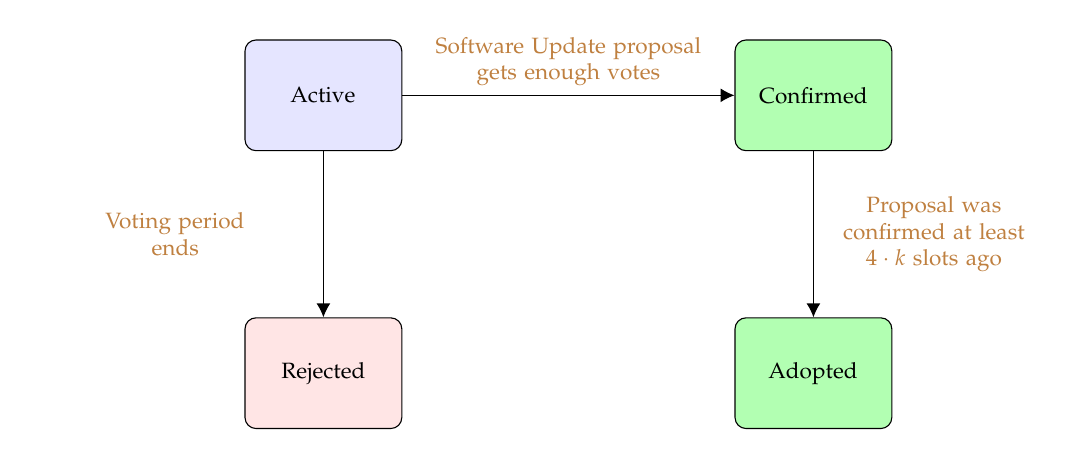
\begin{tikzpicture}[ align = center
                     , node distance = 6em and 12em
                     , text width = 5em
                     , font = \footnotesize
                     , >={Latex[width=0.5em, length=0.5em]}
                     , every node/.style = { rectangle
                                         , rounded corners
                                         , draw = black
                                         , align = center
                                         , minimum height = 4em }
                     ]

  \node (active) [fill = blue!10] {Active};
  \node (rejected) [below = of active, fill = red!10] {Rejected};
  \node (confirmed) [right = of active, fill = green!30] {Confirmed};
  \node (adopted) [below = of confirmed, fill = green!30] {Adopted};

  \tikzset{every node/.style={align=center, text width=10em, text=brown}}

  \draw[->] (active)
  edge node [above] {Software Update proposal\\ gets enough votes}
  (confirmed);

  \draw[->] (active)
  edge node [left] {Voting period \\ends}
  (rejected);

  \draw[->] (confirmed)
  edge node [right, text width=8em]
  {Proposal was confirmed at least $4 \cdot k$ slots ago}
  (adopted);


  \end{tikzpicture}

  \caption{State-transition diagram for software-updates}
  \label{fig:st-diagram-sw-up}
\end{figure}

\clearpage

A sequence of votes can be applied using $\trans{upivotes}{}$ transitions. The
inference rules for them are presented in \cref{fig:rules:apply-votes}. After
applying a sequence of votes, proposals might get confirmed, which means that
they will be added to the set $\var{cps'}$. In such case, the mapping of
application names to their latest version known to the ledger will be updated to
include the information about the confirmed proposals. Note that, unlike
protocol updates, software updates take effect as soon as a proposal is
confirmed (we cannot wait for stability since we need to preserve compatibility
with the existing chain, where there are software update proposals that were
adopted without waiting for $2\cdot k$ slots). In this rule, we also delete the
confirmed id's from the set of registered application update proposals
($\var{raus}$), since this information is no longer needed once the
application-name to software-version map ($\var{avs}$) is updated.

Also note that, unlike the rules of \cref{fig:rules:upi-ec}, we need not remove
other update proposals that refer to the software names whose versions were
changed in $\var{avs_{new}}$. The reason for this is that the range of $\var{raus}$
can contain only one pair of the form $(\var{an}, \wcard, \wcard)$ for any given
application name $\var{an}$ (see Rule~\ref{eq:rule:up-av-validity}).


\begin{figure}[htb]
  \begin{equation}
    \label{eq:rule:apply-votes-base}
    \inference
    {
    }
    {
      {\left(
        \begin{array}{l}
          s_n\\
          \var{dms}
        \end{array}
      \right)}
      \vdash
      \var{us}
      \trans{applyvotes}{\epsilon}
      \var{us}
    }
  \end{equation}
  %
  \nextdef
  %
  \begin{equation}
    \label{eq:rule:apply-votes-ind}
    \inference
    {
      {\left(
        \begin{array}{l}
          s_n\\
          \var{dms}
        \end{array}
      \right)}
      \vdash
      \var{us}
      \trans{applyvotes}{\Gamma}
      \var{us'}
      &
      {\left(
        \begin{array}{l}
          s_n\\
          \var{dms}
        \end{array}
      \right)}
      \vdash
      \var{us'}
      \trans{\hyperref[fig:rules:upi-vote]{upivote}}{v}
      \var{us''}
    }
    {
      {\left(
        \begin{array}{l}
          s_n\\
          \var{dms}
        \end{array}
      \right)}
      \vdash
      \var{us}
      \trans{applyvotes}{\Gamma;v}
      \var{us''}
    }
  \end{equation}
  %
  \nextdef
  %
  \begin{equation}
    \label{eq:rule:upivotes}
    \inference{
      {\left(
        \begin{array}{l}
          s_n\\
          \var{dms}
        \end{array}
      \right)}
      \vdash
      {\left(
          \begin{array}{l}
            (\var{pv}, \var{pps})\\
            \var{fads}\\
            \var{avs}\\
            \var{rpus}\\
            \var{raus}\\
            \var{cps}\\
            \var{vts}\\
            \var{bvs}\\
            \var{pws}
          \end{array}
        \right)}
      \trans{applyvotes}{\Gamma}
      {\left(
          \begin{array}{l}
            (\var{pv'}, \var{pps'})\\
            \var{fads'}\\
            \var{avs'}\\
            \var{rpus'}\\
            \var{raus'}\\
            \var{cps'}\\
            \var{vts'}\\
            \var{bvs'}\\
            \var{pws'}
          \end{array}
      \right)}\\
      %
      {\begin{array}{r@{~\leteq~}l}
        \var{cfm_{raus}} & \dom~(cps') \restrictdom \var{raus'}\\
        \var{avs_{new}} & \{ \var{an} \mapsto (\var{av}, \var{s_n}, m)
        \mid (\var{an}, \var{av}, m) \in \var{cfm_{raus}} \}
      \end{array}}
    }{
      {\left(
        \begin{array}{l}
          s_n\\
          \var{dms}
        \end{array}
      \right)}
      \vdash
      {\left(
          \begin{array}{l}
            (\var{pv}, \var{pps})\\
            \var{fads}\\
            \var{avs}\\
            \var{rpus}\\
            \var{raus}\\
            \var{cps}\\
            \var{vts}\\
            \var{bvs}\\
            \var{pws}
          \end{array}
      \right)}
      \trans{upivotes}{\Gamma}
      {\left(
          \begin{array}{l}
            (\var{pv'}, \var{pps'})\\
            \var{fads'}\\
            \var{avs'} \unionoverrideRight \var{avs_{new}}\\
            \var{rpus'}\\
            \dom~(cps') \subtractdom \var{raus'}\\
            \var{cps'}\\
            \var{vts'}\\
            \var{bvs'}\\
            \var{pws'}
          \end{array}
      \right)}
    }
  \end{equation}
  \caption{Applying multiple votes on update-proposals rules}
  \label{fig:rules:apply-votes}
\end{figure}
\clearpage

The interface rule for protocol-version endorsement makes use of the
$\trans{upend}{}$ transition, where we set the threshold for proposal adoption
to: the number of genesis keys ($\var{ngk}$) times the minimum proportion of
genesis keys that need to endorse an update proposal for it to become a
candidate for adoption (given by the protocol parameter $\var{upAdptThd}$). In
addition, the unconfirmed proposals that are older than $u$ blocks are removed
from the parts of the state that hold:
\begin{itemize}
\item the registered protocol and software update proposals,
\item the votes associated with the proposals,
\item the set of endorsement-key pairs, and
\item the block number in which proposals where added.
\end{itemize}

In Rule~\ref{eq:rule:upi-pend}, the set of proposal id's $\var{pid_{keep}}$
contains only those proposals that haven't expired yet or that are confirmed.
Once a proposal $\var{up}$ is confirmed, it is removed from the set of
confirmed proposals ($\var{cps}$) when a new a protocol version gets adopted
(see Rule~\ref{eq:rule:upi-ec-pv-change}).
%
The set of endorsement-key pairs is cleaned here as well as in the epoch change
rule (Rule~\ref{eq:rule:upi-ec-pv-change}). The reason for this is that this set grows at
each block, and it can get considerably large if no proposal gets adopted at
the end of an epoch.

\begin{figure}[htb]
  \begin{equation}
    \label{eq:rule:upi-pend}
    \inference
    {
      \var{upAdptThd} \mapsto q \in \var{pps} \\
      \left({
        \begin{array}{l}
          s_n\\
          \floor{q \cdot \var{ngk}}\\
          \var{dms}\\
          \var{cps}\\
          \var{rpus}
        \end{array}
      }\right)
      \vdash
      {
        \left(
          \begin{array}{l}
            \var{fads}\\
            \var{bvs}
          \end{array}
        \right)
      }
      \trans{\hyperref[fig:rules:up-end]{upend}}{(\var{bv}, \var{vk})}
      {
        \left(
          \begin{array}{l}
            \var{fads'}\\
            \var{bvs'}
          \end{array}
        \right)
      }\\
      \var{upropTTL} \mapsto u \in \var{pps}\\
      {
        \begin{array}{r@{~\leteq~}l}
          \var{pids_{keep}} & \dom~(pws \restrictrange [s_n - u, ..]) \cup \dom~\var{cps}\\
          \var{vs_{keep}} & \dom~(\range~\var{rpus'})\\
          \var{rpus'} & \var{pids_{keep}} \restrictdom \var{rpus}
        \end{array}
      }
    }
    {
      {\left(
        \begin{array}{l}
          s_n\\
          \var{dms}
        \end{array}
      \right)}
      \vdash
      {
        \left(
          \begin{array}{l}
            (\var{pv}, \var{pps})\\
            \var{fads}\\
            \var{avs}\\
            \var{rpus}\\
            \var{raus}\\
            \var{cps}\\
            \var{vts}\\
            \var{bvs}\\
            \var{pws}
          \end{array}
        \right)
      }
      \trans{upiend}{(\var{bv}, \var{vk})}
      {
        \left(
          \begin{array}{l}
            (\var{pv}, \var{pps})\\
            \var{fads'}\\
            \var{avs}\\
            \var{rpus'}\\
            \var{pids_{keep}} \restrictdom \var{raus}\\
            \var{cps}\\
            \var{pids_{keep}} \restrictdom \var{vts}\\
            \var{vs_{keep}}  \restrictdom \var{bvs'}\\
            \var{pids_{keep}} \restrictdom \var{pws}
          \end{array}
        \right)
      }
    }
  \end{equation}
  \caption{Proposal endorsement rules}
  \label{fig:rules:upi-pend}
\end{figure}

\clearpage

Rule~\ref{eq:rule:upi-ec-pv-change} models how the protocol-version and its
parameters are changed depending on an epoch change signal.
%
On an epoch change, this rule will pick a candidate that gathered enough
endorsements at least $4 \cdot k$ slots ago. If a protocol-version candidate
cannot gather enough endorsements $4 \cdot k$ slots before the end of an epoch,
the proposal can only be adopted in the next epoch. The reason for the $4 \cdot
k$ slot delay is to allow a period between knowing when a proposal will be
adopted, and the event of its being adopted. Since update proposals can and will
make large changes to the way the chain operates, it is useful to be able to
guarantee a window in which it is known that no update will take place.
%
Figure~\ref{fig:up-confirmed-too-late} shows an example of a proposal being
confirmed too late in an epoch, where it is not possible to get enough
endorsements in the remaining window. In this Figure we take $k = 2$, and we
assume $4$ endorsements are needed to consider a proposal as candidate for
adoption.
%
Note that, in the final state, we use union override to define the updated
parameters ($\var{pps} \unionoverrideRight \var{pps'}$). This is because candidate
proposal might only update some parameters of the protocol.

In Rule~\ref{eq:rule:upi-ec-pv-change}, when a new proposal gets adopted, all
the state components that refer to protocol update proposals get emptied. The
reason for this is that at the moment of registering a proposal, we evaluated
it in a state where the protocol parameters that we used for this are no longer
up to date (see for instance \cref{eq:func:can-update}). For instance, assume
we register a proposal $\var{up}$ which only changes the maximum transaction
size to $x$, and the current block size is set to $x + 1$. Then,
$\fun{canUpdate}$ holds, since the maximum transaction size is less than the
maximum block size. If now a new proposal gets adopted that changes the maximum
block size to $x - 1$, then this invalidates $\var{up}$ since $\fun{canUpdate}$
no longer holds.
%

If there are no candidates for adoption, then the state variables remain
unaltered (Rule~\ref{eq:rule:upi-ec-pv-unchanged}).

Also note that the registered software-update proposals need not be cleaned
here, since this is done either when a proposal gets confirmed or when it
expires.

\begin{figure}[htb]
  \begin{equation}
    \label{eq:rule:pvbump-change-epoch-only}
    \inference
    {
      [.., s_n - 4 \cdot k] \restrictdom \var{fads} = \epsilon
    }
    {
      {\left(\begin{array}{l}
         s_n\\
         \var{fads}
       \end{array}\right)}
      \vdash
      {
        \left(
          \begin{array}{l}
            \var{pv}, \var{pps}\\
          \end{array}
        \right)
      }
      \trans{pvbump}{}
      {
        \left(
          \begin{array}{l}
            \var{pv}, \var{pps}\\
          \end{array}
        \right)
      }
    }
  \end{equation}
  \nextdef
  \begin{equation}
    \label{eq:rule:pvbump-change}
    \inference
    {
      \wcard ; (\wcard , (\var{pv_c}, \var{pps_c})) \leteq [.., s_n - 4 \cdot k] \restrictdom \var{fads}
    }
    {
      {\left(\begin{array}{l}
         s_n\\
         \var{fads}
       \end{array}\right)}
      \vdash
      {
        \left(
          \begin{array}{l}
            \var{pv}, \var{pps}\\
          \end{array}
        \right)
      }
      \trans{pvbump}{}
      {
        \left(
          \begin{array}{l}
            \var{pv_c}, \var{pps_c}\\
          \end{array}
        \right)
      }
    }
  \end{equation}
  \caption{Protocol version bump rules}
  \label{fig:rules:pvbump}
\end{figure}

\begin{figure}[htb]
  \begin{equation}
    \label{eq:rule:upi-ec-pv-unchanged}
    \inference
    {
      {\left(\begin{array}{l}
         \fun{firstSlot}~e_n\\
         \var{fads}
       \end{array}\right)}
      \vdash
      {
        \left(
          \begin{array}{l}
            \var{pv}, \var{pps}
          \end{array}
        \right)
      }
      \trans{\hyperref[fig:rules:pvbump]{pvbump}}{}
      {
        \left(
          \begin{array}{l}
            \var{pv'}, \var{pps'}\\
          \end{array}
        \right)
      } &\var{pv} = \var{pv'}
    }
    {
      (e_n)
      \vdash
      {
        \left(
          \begin{array}{l}
            (\var{pv}, \var{pps})\\
            \var{fads}\\
            \var{avs}\\
            \var{rpus}\\
            \var{raus}\\
            \var{cps}\\
            \var{vts}\\
            \var{bvs}\\
            \var{pws}
          \end{array}
        \right)
      }
      \trans{upiec}{}
      {
        \left(
          \begin{array}{l}
            (\var{pv}, \var{pps})\\
            \var{fads}\\
            \var{avs}\\
            \var{rpus}\\
            \var{raus}\\
            \var{cps}\\
            \var{vts}\\
            \var{bvs}\\
            \var{pws}
          \end{array}
        \right)
      }
    }
  \end{equation}
  \nextdef
  \begin{equation}
    \label{eq:rule:upi-ec-pv-change}
    \inference
    {
      {\left(\begin{array}{l}
         \fun{firstSlot}~e_n\\
         \var{fads}
       \end{array}\right)}
      \vdash
      {
        \left(
          \begin{array}{l}
            \var{pv}, \var{pps}\\
          \end{array}
        \right)
      }
      \trans{\hyperref[fig:rules:pvbump]{pvbump}}{}
      {
        \left(
          \begin{array}{l}
            \var{pv'}, \var{pps'}\\
          \end{array}
        \right)
      }
      & \var{pv} \neq \var{pv'}
    }
    {
      (e_n)
      \vdash
      {
        \left(
          \begin{array}{l}
            \var{(\var{pv}, \var{pps})}\\
            \var{fads}\\
            \var{avs}\\
            \var{rpus}\\
            \var{raus}\\
            \var{cps}\\
            \var{vts}\\
            \var{bvs}\\
            \var{pws}
          \end{array}
        \right)
      }
      \trans{upiec}{}
      {
        \left(
          \begin{array}{l}
            (\var{pv'}, \var{pps'})\\
            \epsilon\\
            \var{avs}\\
            \emptyset\\
            \emptyset\\
            \emptyset\\
            \emptyset\\
            \emptyset\\
            \emptyset\\
          \end{array}
        \right)
      }
    }
  \end{equation}
  \caption{Block version adoption on epoch change rules}
  \label{fig:rules:upi-ec}
\end{figure}

\begin{figure}[htb]
  \centering
  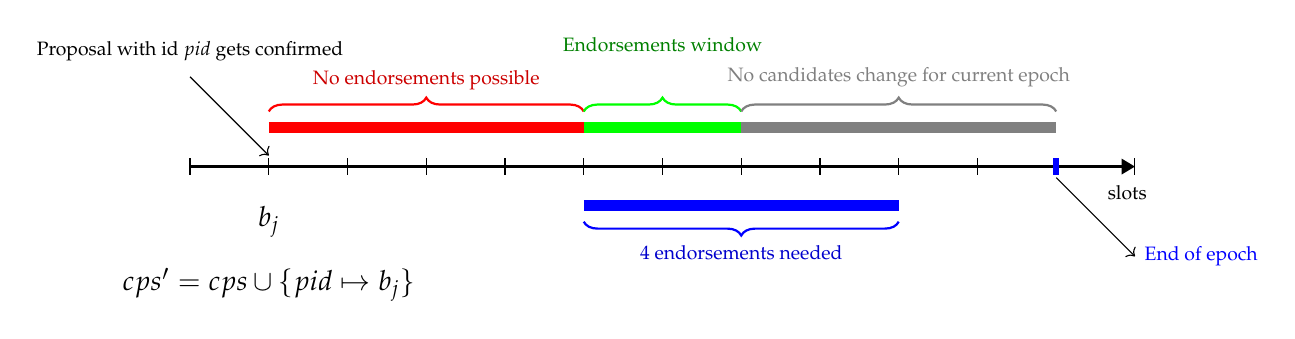
\begin{tikzpicture}
    %%
    %% Macros used in this picture
    %%
    %
    % Number of slots
    \pgfmathsetmacro{\nrSlots}{12}
    % Slot in which the proposal gets confirmed
    \pgfmathsetmacro{\cSlot}{1}
    % Our special K.
    \pgfmathsetmacro{\K}{4}
    % Epoch end.
    \pgfmathsetmacro{\eend}{11}
    % Number of positive votes needed
    \pgfmathsetmacro{\votes}{4}

    % Draw the horizontal line
    \draw[thick, -Triangle] (0,0) -- (\nrSlots,0)
    node[font=\scriptsize,below left=3pt and -8pt]{slots};

    % % draw vertical lines
    \foreach \x in {0,1,...,\nrSlots}
    \draw (\x cm, 3pt) -- (\x cm, -3pt);

    % Add a label to with the block number in which the proposal got confirmed.
    \node at (\cSlot, -.7) {$b_j$};

    % Update in cps
    \node at (\cSlot, -1.5) {$\var{cps'} = \var{cps} \cup \{ \var{pid} \mapsto b_j \}$};

    % The no-endorsements red bar.
    \draw[red, line width=4pt] (\cSlot, .5) -- +(\K, 0);

    % Brace above the no-endorsement window bar.
    \draw[thick, red, decorate, decoration={brace, amplitude=5pt}]
    (\cSlot, .7) -- +(\K, 0)
    node[black!20!red, midway, above=4pt, font=\scriptsize] {No endorsements possible};

    % The endorsements window.
    \coordinate (ewStart) at (\cSlot + \K, .5);
    \coordinate (ewEnd) at ($(\eend - \K, .5)$);
    \draw[green, line width=4pt]
    (ewStart) -- (ewEnd);

    % Brace above the endorsements window
    \coordinate (ewStartB) at ($(ewStart) + (0, 0.2)$);
    \coordinate (ewEndB) at ($(ewEnd) + (0, 0.2)$);
    \draw[thick, green, decorate, decoration={brace, amplitude=5pt}]
    (ewStartB) -- (ewEndB)
    node[black!50!green, midway, above=18pt, font=\scriptsize] {Endorsements window};

    % The no-candidates change window.
    \coordinate (nccStart) at (\eend - \K, .5);
    \coordinate (nccEnd) at ($(\eend, .5)$);
    \draw[gray, line width=4pt]
    (nccStart) -- (nccEnd);

    % Brace above the no-candidates change window.
    \coordinate (nccStartB) at ($(nccStart) + (0, 0.2)$);
    \coordinate (nccEndB) at ($(nccEnd) + (0, 0.2)$);
    \draw[thick, gray, decorate, decoration={brace, amplitude=5pt}]
    (nccStartB) -- (nccEndB)
    node[gray, midway, above=5pt, font=\scriptsize] {No candidates change for current epoch};


    % The 2k before end-of-epoch window.
    \coordinate (beeStart) at (\cSlot + \K, -.5);
    \coordinate (beeEnd) at ($(\cSlot + \K + \votes, -.5)$);
    \draw[blue, line width=4pt]
    (beeStart) -- (beeEnd);

    % Brace on above the 2k before end-of-epoch window.
    \coordinate (beeStartB) at ($(beeStart) - (0, 0.2)$);
    \coordinate (beeEndB) at ($(beeEnd) - (0, 0.2)$);
    \draw[thick, blue, decorate, decoration={brace, amplitude=5pt}]
    (beeEndB) -- (beeStartB)
    node[black!20!blue, midway, below=5pt, font=\scriptsize] {$\votes$ endorsements needed};

    \draw[blue, line width=2pt] (\eend, 3pt) -- (\eend, -3pt);

    \draw[<-] (\cSlot, 4pt) -- +(-1, 1)
    node [above=2pt, black, font=\scriptsize]
    {Proposal with id $\var{pid}$ gets confirmed};

    \draw[->] (\eend, -4pt) -- +(1, -1)
    node[right, blue, font=\scriptsize] {End of epoch};
  \end{tikzpicture}
  \caption{An update proposal confirmed too late}
  \label{fig:up-confirmed-too-late}
\end{figure}

Figure~\ref{fig:st-diagram-pt-up} shows the different states a protocol-update
proposal can be in, and what causes the transitions between them.

\begin{figure}[ht]
  \centering
  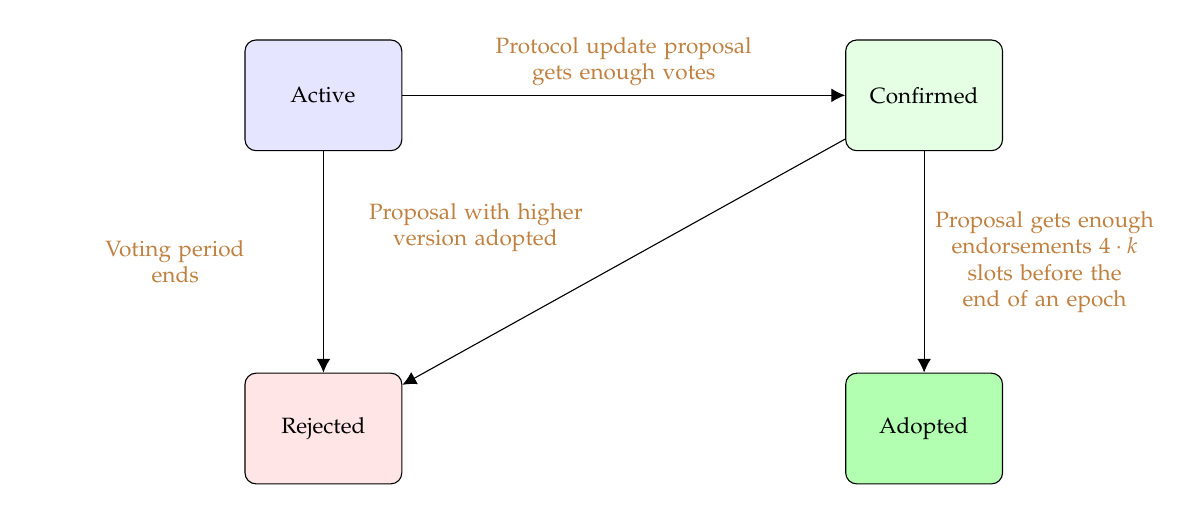
\begin{tikzpicture}[ align = center
                     , node distance = 8em and 16em
                     , text width = 5em
                     , font = \footnotesize
                     , >={Latex[width=0.5em, length=0.5em]}
                     , every node/.style = { rectangle
                                         , rounded corners
                                         , draw = black
                                         , align = center
                                         , minimum height = 4em }
                     ]

  \node (active) [fill = blue!10] {Active};
  \node (rejected) [below = of active, fill = red!10] {Rejected};
  \node (confirmed) [right = of active, fill = green!10] {Confirmed};
  \node (adopted) [below = of confirmed, fill = green!30] {Adopted};

  \tikzset{every node/.style={align=center, text width=10em, text=brown}}

  \draw[->] (active)
  edge node [above] {Protocol update proposal\\ gets enough votes}
  (confirmed);

  \draw[->] (active)
  edge node [left] {Voting period \\ends}
  (rejected);

  \draw[->] (confirmed)
  edge node [above left]
  {Proposal with higher version adopted}
  (rejected);

  \draw[->] (confirmed)
  edge node [right, text width=8em]
  {Proposal gets enough endorsements $4 \cdot k$ slots before the end of an epoch}
  (adopted);

  \end{tikzpicture}

  \caption{State-transition diagram for protocol-updates}
  \label{fig:st-diagram-pt-up}
\end{figure}


\newcommand{\Val}{\fun{Val}}
\newcommand{\POV}[1]{\ensuremath{\mathsf{PresOfVal}(\mathsf{#1})}}
\newcommand{\DBE}[2]{\ensuremath{\mathsf{DBE}({#1},~{#2})}}
\newcommand{\DGO}[2]{\ensuremath{\mathsf{DGO}({#1},~{#2})}}
\newcommand{\transtar}[2]{\xlongrightarrow[\textsc{#1}]{#2}\negthickspace^{*}}

\section{Properties}
\label{sec:properties}

This section describes the properties that the ledger should have. The goal is to
to include these properties in the executable specification to enable e.g.
property-based testing or formal verification.

% TODO - the hand proofs of preservation of ada and non-negative deposit
% pot are woefully out of date, mostly due to the removal of decaying deposits.
%
\subsection{Preservation of Value}
\label{sec:preservation-of-value}

As visualized in Figure~\ref{fig:fund-preservation},
the total amount of lovelace in any given chain state
$\var{s}\in\ChainState$ is completely contained within the values of the six
variables:

\begin{tabular}{||l|l|l|l||}\hline\hline

  \textbf{Variable} & \textbf{Name in Figure~\ref{fig:fund-preservation}}
                    & \textbf{Nesting Inside Chain State} & \textbf{Kind} \\ \hline
  utxo & circulation & s.nes.es.ls.utxoSt & Map over Lovelace Values  \\ \hline
  deposits & deposits &  s.nes.es.ls.utxoSt & Lovelace Value ($\Coin$) \\ \hline
  fees & fees &  s.nes.es.ls.utxoSt & Lovelace Value ($\Coin$) \\ \hline
  rewards & reward accounts & s.nes.es.ls.dpstate.dstate  & Lovelace Value ($\Coin$)  \\ \hline
  treasury & treasury &  s.nes.es.acnt  & Lovelace Value ($\Coin$) \\ \hline
  reserves & reserves & s.nes.es.acnt & Map over Lovelace Values \\ \hline
  \hline
\end{tabular}

\noindent
Notice that $\var{deposits}$, $\var{fees}$, $\var{treasury}$, and $\var{reserves}$
are all single lovelace values, while $\var{utxo}$, and $\var{rewards}$ are
maps whose values are lovelace.

We define the \emph{Lovelace Value} of a given chain state as:
\begin{definition}[Lovelace Value]
  \label{def:val}
  \begin{equation*}
    \Val(s~\in~\var{State}) =
        \Val(\var{utxo}) +
            \Val(\var{deposits}) +
            \Val(\var{fees}) +
            \Val(\var{reserves}) +
            \Val(\var{treasury}) +
            \Val(\var{rewards})
  \end{equation*}
  where
  \begin{equation*}
      \Val(x \in \Coin) = x
  \end{equation*}
  \begin{equation*}
      \Val((\wcard\mapsto (y \in \Coin))^{*}) = \sum y
  \end{equation*}
\end{definition}

\noindent
For any state that is used in a given subtransition of $\mathsf{CHAIN}$,
we define $\Val{}$ in an analogous way, setting the value of any variable that is not explicitly
represented in the state to zero.
For example, given $\var{utxoSt}\in\UTxOState$,
\begin{equation*}
  \Val(\var{utxoSt}) =
  \left(\sum_{\wcard\mapsto(\wcard,~v)\in\var{utxo}}v\right) + \var{deposits} + \var{fees}
\end{equation*}

\noindent
The key property that we want to prove is that no semantic transition changes the value that
is captured in the state ($\Val{s}$).
This property is easy to state: intuitively,
the \emph{Lovelace Value}before the transition is the same as the
\emph{Lovelace Value} after that transition.

\begin{theorem}[Preservation of Value]
  \label{thm:chain-pres-of-value}
  For all environments $e$, blocks $b$, and states $s$, $s'$, if
  \begin{equation*}
    e\vdash s\trans{\hyperref[fig:rules:chain]{chain}}{b}s'
  \end{equation*}
  then
  \begin{equation*}
    \Val(s) = \Val(s')
  \end{equation*}
\end{theorem}

\noindent
We will prove the soundness of Theorem~\ref{thm:chain-pres-of-value} via a few lemmas.

\begin{lemma}
  \label{lemma:value-sum-pres-1}
  For any mapping $m:A\mapsto\Coin$ and set $s\in\powerset{A}$,
  \begin{equation*}
    \Val(\var{m}) = \Val(s\subtractdom m) + \Val(s\restrictdom m)
  \end{equation*}
\end{lemma}
\begin{proof}
  easy
\end{proof}

\begin{lemma}
  \label{lemma:value-sum-pres-2}
  For any mappings $m_1, m_2:A\mapsto\Coin$,
  if $\dom{m_1}\cap\dom{m_2}=\emptyset$,
  then
  \begin{equation*}
    \Val(m_1\cup m_2) = \Val(m_1) + \Val(m_2)
  \end{equation*}
\end{lemma}
\begin{proof}
  easy
\end{proof}

\begin{lemma}
  \label{lemma:utxo-pres-of-value}
  For all environments $e$, transactions $t$, and states $s$, $s'$, if
  \begin{equation*}
    e\vdash s\trans{\hyperref[fig:rules:utxo-shelley]{utxo}}{t}s'
  \end{equation*}
  then
  \begin{equation*}
    \Val(s) + w = \Val(s')
  \end{equation*}
  where $w = \fun{wbalance}~(\fun{txwdrls}~{t})$.
\end{lemma}

\begin{proof}
  The proof is essentially unfolding the definition of the predicate
  \begin{equation}
    \label{cons-is-prod}
    \consumed{pp}{utxo}{t} = \produced{pp}{stpools}{t}
  \end{equation}
  and applying a little algebra.
%
If we let:
  \begin{equation*}
    \begin{array}{r@{~=~}l}
      k & \keyRefunds{pp}{stkCreds}{t} \\
      f & \txfee{t} \\
      d & \totalDeposits{pp}{stpools}{(\txcerts{t})} \\
    \end{array}
  \end{equation*}
  then equation~\ref{cons-is-prod} can be rewritten as:
  \begin{equation*}
    \Val(\txins{t} \restrictdom{\var{utxo}}) + w + k = \Val(\outs{t}) + f + d
  \end{equation*}
  where $\outs{}$ is defined in Figure~\ref{fig:functions:utxo} and returns a value of type $\UTxO$.
  Therefore, moving $k$ to the right and adding $\txins{t} \subtractdom{\var{utxo}}$ to each side,
  \begin{equation*}
    \Val(\txins{t} \restrictdom{\var{utxo}}) + \Val(\txins{t} \subtractdom{\var{utxo}}) + w
    = \Val(\outs{t}) + f + d - k + \Val(\txins{t} \subtractdom{\var{utxo}})
  \end{equation*}
  (Though not needed for the proof at hand,
  note that $d-k$ is non-negative since the deposits will always be large enough to cover
  the current obligation. See Theorem~\ref{thm:non-neg-deposits}.)
%
  It then follows that:
  \begin{equation*}
    \begin{array}{r@{~=~}lr}
      \Val(\var{utxo}) + w
    & \Val(\outs{t}) + f + d - k + \Val(\txins{t} \subtractdom{\var{utxo}})
    & \text{(by Lemma~\ref{lemma:value-sum-pres-1})}
    \\
    & \Val((\txins{t} \subtractdom{\var{utxo}})\cup\outs{t}) + (d - k) + f
    & \text{(by Lemma~\ref{lemma:value-sum-pres-2})}
    \end{array}
  \end{equation*}
  Note that in order to apply Lemma~\ref{lemma:value-sum-pres-2} above,
  it must be true that $(\txins{t} \subtractdom{\var{utxo}})$ and $(\outs{t})$
  have disjoint domains, which follows from the uniqueness of the transaction IDs.

  Therefore, by adding the deposits and fees from $s$ to the equality above,
  it follows that $\Val(s) + w = \Val(s')$.
\end{proof}

\begin{lemma}
  \label{lemma:deleg-pres-of-value}
  For all environments $e$, transactions $c$, and states $s$, $s'$, if
  \begin{equation*}
    e\vdash s\trans{\hyperref[fig:delegation-rules]{deleg}}{c}s'
  \end{equation*}
  then
  \begin{equation*}
    \Val(s) = \Val(s')
  \end{equation*}
\end{lemma}

\begin{proof}
  The only variable with value in this transition is \var{rewards}.
  Only two of the rules in $\mathsf{DELEG}$ can change \var{rewards},
  namely $\mathsf{Deleg{-}Reg}$ and $\mathsf{Deleg{-}Dereg}$.
  However, $\mathsf{Deleg{-}Reg}$ only adds a zero value,
  and $\mathsf{Deleg{-}Dereg}$ only removes a zero value.
\end{proof}

\begin{lemma}
  \label{lemma:delegs-pres-of-value}
  For all environments $e$, certificates $\Gamma$, and states $s$, $s'$, if
  \begin{equation*}
    e\vdash s\trans{\hyperref[fig:rules:delegation-sequence]{delegs}}{\Gamma}s'
  \end{equation*}
  then
  \begin{equation*}
    \Val(s) = \Val(s') + w
  \end{equation*}
  where $w = \fun{wbalance}~(\fun{txwdrls}~{t})$,
  and $t$ is the transaction in the environment $e$.
\end{lemma}

\begin{proof}
  The proof is by induction on the length of $\Gamma$.
  Note that the only variable with value in this transition is \var{rewards}.

  \vspace{2ex}
  \noindent
  \emph{In the base case}, we look at the rule $\mathsf{Seq{-}delg{-}base}$.
  Since $\var{wdrls}\subseteq\var{rewards}$, then
  $\var{rewards} = \var{wdrls}\cup\var{(\var{rewards}\setminus\var{wdrls})}$.
%
  Therefore
  \begin{equation*}
    \begin{array}{r@{~=~}lr}
      \Val{(\var{rewards})}
      & \Val{(\var{rewards}\setminus\var{wdrls})} + \Val{(\var{wdrls})}
      & \text{by Lemma~\ref{lemma:value-sum-pres-2}}
      \\
      & \Val{(\var{rewards}\setminus\var{wdrls})} + w
      & \text{by definition}
      \\
      & \Val\left(\var{rewards}\unionoverrideRight\{(w, 0) \mid w \in \dom \var{wdrls}\}\right) + w
    \end{array}
  \end{equation*}
  Therefore $\Val(s) = \Val(s')$.

  \vspace{2ex}
  \noindent
  \emph{In the inductive case}, we look at the rule $\mathsf{Seq{-}delg{-}ind}$.
  In this case, the lemma then follows directly from Lemma~\ref{lemma:deleg-pres-of-value}.
\end{proof}

\begin{lemma}
  \label{lemma:poolreap-pres-of-value}
  For all environments $e$, epoch $\epsilon$, and states $s$, $s'$, if
  \begin{equation*}
    e\vdash s\trans{\hyperref[fig:rules:pool-reap]{poolreap}}{\epsilon}s'
  \end{equation*}
  then
  \begin{equation*}
    \Val(s) = \Val(s')
  \end{equation*}
\end{lemma}

\begin{proof}
  The $\mathsf{POOLREAP}$ value is contained in
  $\var{deposits}$, $\var{treasury}$, and $\var{rewards}$.
  Notice that $\var{unclaimed}$ is added to $\var{treasury}$
  and subtracted from the $\var{deposits}$.
  Moreover, $\var{refunded}$ is subtracted from $\var{deposits}$.
  (Note that $\var{deposits}-(\var{unclaimed}+\var{refunded})$
  is non-negative by Theorem~\ref{thm:non-neg-deposits}.)
  It therefore suffices to show that
  \begin{equation*}
    \begin{array}{r@{~=~}l}
    \Val(\var{rewards}\unionoverridePlus\var{refunds})
    & \Val(\var{rewards}) + \Val(\var{refunds})
    \\
    & \Val(\var{rewards}) + \var{refunded}
    \end{array}
  \end{equation*}
  But this is clear from the definition of $\unionoverridePlus$.
\end{proof}

\begin{lemma}
  \label{lemma:ru-pres-of-value}
  For every $(\Delta t,~\Delta r,~\var{rs},~\Delta f)$ in the range of $\fun{createRUpd}$,
  \begin{equation*}
    \Delta t + \Delta r + \Val(rs) + \Delta f = 0
  \end{equation*}
\end{lemma}

\begin{proof}
  In the definition of $\fun{createRUpd}$ in Figure~\ref{fig:functions:reward-update-creation},
  We see that:
  \begin{equation*}
    \begin{array}{r@{~=~}l}
      \var{rewardPot} & \var{feeSS} + \Delta r \\
      \var{R} & \var{rewardPot} - \Delta t_1 \\
      \Delta t_2 & R - \Val(\var{rs})\\
      \Delta t & \Delta t_1 + \Delta t_2 \\
    \end{array}
  \end{equation*}
  Therefore
  \begin{equation*}
    \begin{array}{r@{~=~}l}
      (\var{feeSS} + \Delta r) & \var{rewardPot} = R + \Delta t_1 = \Delta t_2 + \Val(rs) + \Delta t_1  \\
      0 & (\Delta t_1 + \Delta t_2 ) - \Delta r + \Val(rs)- \var{feeSS} \\
      0 & \Delta t - \Delta r + \Val(rs)- \var{feeSS} \\
    \end{array}
  \end{equation*}
  It then suffices to notice that $\fun{createRUpd}$ returns
  $(\Delta t,-~\Delta r,~\var{rs},~-\var{feeSS})$.
\end{proof}

\noindent

Note that Lemma~\ref{lemma:ru-pres-of-value} is not strictly need for the proof of
Theorem~\ref{thm:chain-pres-of-value}, since the $\mathsf{NEWEPOCH}$ transition
requires that $\Delta t + \Delta r + \Val(rs) + \Delta f = 0$ holds.
It does, however, give us confidence that the $\mathsf{CHAIN}$ transition can proceed.

We are now ready to prove Theorem~\ref{thm:chain-pres-of-value}.

\begin{proof}
  For a given transition $\mathsf{TR}$, let \POV{TR}
  be the statement:

  \begin{tabular}{l}
    for all environments $e$, signals $\sigma$, and states $s$, $s'$,
    $$
    $e\vdash s\trans{tr}{\sigma}s'~\implies~\Val(s) = \Val(s')$.
    $$
  \end{tabular}

  \noindent
  Our goal is to prove \POV{CHAIN}.
  Lemmas~\ref{lemma:utxo-pres-of-value} and \ref{lemma:delegs-pres-of-value} imply \POV{LEDGER},
  since $\mathsf{UTXOW}$ transforms state exactly as $\mathsf{UTXO}$ does.
  \POV{LEDGERS} then follows by straightforward induction on the length of $\Gamma$:
  the base case is trivial;
  and the inductive case follows directly from \POV{LEDGER}.
%
  \POV{SNAP} holds trivially, since it contains no value.
  Similarly, \POV{NEWPP} holds since $\var{diff}$ is added to $\var{reserves}$
  and subtracted from $\var{deposits}$.
  Therefore \POV{EPOCH} holds by Lemma~\ref{lemma:poolreap-pres-of-value}.
  \POV{MIR} holds since
  $\Val{i_{rwd}'}=\var{tot}$ in Figure~\ref{fig:rules:mir}.
  Morover, \POV{NEWEPOCH} holds in the presence of $\fun{applyRUpd}$
  since the transition requires $\Delta t + \Delta r + \Val(rs) + \Delta f = 0$.
  \POV{CHAIN} easily follows from this.
\end{proof}

\subsection{Non-negative Deposit Pot}  % TODO - this section is out of date due to no decaying deposits
\label{sec:non-negative-deposit-pot}

The \emph{deposit pot} (the variable $\var{deposits}$ in the UTxO State)
represents the amount of \emph{lovelace} that is set aside by the system as a whole for refunding deposits.
Deposits are added to this pot, which then decays exponentially over time,
and is also depleted by any refunded deposits.
At an epoch boundary, the decayed parts of any deposits (including, possibly, deposits for any transactions that will complete in future epochs)
will be distributed as additional \emph{rewards}, as described in~\cite{delegation_design}.
Since $\var{deposits}$ is only used to record the value of future refunds or rewards whose costs have
already been incurred, both it and any reward value will always be non-negative.
Note that there are two types of deposits which are recorded in the same pot: those for stake keys; and those for stake pools.
Stake keys are deregistered in the slot in which the deregistration certificates
is processed. Stake pools, however, are staged for retirement on epoch boundaries.
%
The following theorem ensures that the deposit pot is properly maintained
and will always be large enough to meet all of its obligations.


\begin{figure}[h!]
  \begin{tabular}{||l|l|l|l||}\hline\hline

    \textbf{Variable} & \textbf{Value}
                      & \textbf{Nesting Inside Chain State} & \textbf{Kind} \\ \hline
    deposits & 0 &  s.nes.es.ls.utxoSt & $\Coin$ \\ \hline
    stkCreds & $\emptyset$ & s.nes.es.ls.dpstate.dstate.stkCreds
             & $\StakeCreds$ ($\Credential\mapsto\Slot$)  \\ \hline
    stpools & $\emptyset$ & s.nes.es.ls.dpstate.pstate.stpools
            & $\StakePools$ ($\KeyHash\mapsto\Slot$)  \\ \hline
  \end{tabular}
  \caption{Initial Chain State}
  \end{figure}

\begin{theorem}[Non-negative Deposit Pot]
  \label{thm:non-neg-deposits}
  Let $n\in\N$ and $c_0\in\ChainState$ be a chain state in which $\var{deposits} ~=~0$, $\var{stkCreds}~=~\emptyset$ and $\var{stPools}~=~\emptyset$, as shown above:
%  \\~\\
  If
  \begin{equation*}
    s_0\vdash c_0\trans{\hyperref[fig:rules:chain]{chain}}{b_0}c_1,~~
    s_1\vdash c_1\trans{\hyperref[fig:rules:chain]{chain}}{b_1}c_2,~~
    \ldots,~~
    s_n\vdash c_n\trans{\hyperref[fig:rules:chain]{chain}}{b_n}c_{n+1},~~n \ge 0
  \end{equation*}
  is a sequence of valid $\mathsf{CHAIN}$ transitions,
  then $\forall i, 0 \le i \le n, \var{deposits} ~(c_{n+1}) \ge 0$.
\end{theorem}

\begin{proof}

  We will prove a slightly stronger condition, namely that some stronger invariants hold
  most of the time, and that when they do fail to hold, then $\var{deposits}$ is still non-negative.
  These stronger invariants will require a few additional definitions.
%
  Given a slot $s$, let $\ell(s)$ be the first slot of the epoch that $s$ occurs in,
  that is $\ell = \fun{firstSlot}\circ\fun{epoch}$.
  Given a mapping $m\in\mathsf{T}\to\Slot$ and a slot $s\in\Slot$,
  let $\fun{sep}$ be the function that separates $m$ into two maps,
  those whose value is strictly less than $s$ and those whose value is at least $s$.
  So,
  \begin{equation*}
    \fun{sep}~m~s = \forall x\mapsto t~\in~m,~~
    \left(\{x\mapsto t~\mid~t<s\},~\{x\mapsto t~\mid~t\geq s\}\right)
  \end{equation*}


  \noindent
  If we assume that the \emph{protocol parameters}, $pp$, are fixed\footnote{Note that the
    protocol parameters can only change in the $\mathsf{NEWPP}$ transition.}, then we can provide convenience functions
  $R_c$ and $R_p$ for the \emph{stake credential} and \emph{stake pool} refunds, respectively:
  \begin{equation*}
    \begin{array}{r@{~=~}l}
      R_c~s_0~s_1 & \refund{d_{val}}{d_{min}}{\lambda_d}{s_1-s_0} \\
      R_p~s_0~s_1 & \refund{p_{val}}{p_{min}}{\lambda_p}{s_1-s_0} \\
    \end{array}
  \end{equation*}
  where $d_{val}$, $d_{min}$, $\lambda_d$, $p_{val}$, $p_{min}$, $\lambda_p$
  are the protocol parameter values from $pp$, and $\fun{refund}$ is defined in
  Figure~\ref{fig:functions:deposits-refunds}.
  We let \DBE{c}{s} (``Deposits (precisely) Big Enough"), be the following property:
  \begin{equation}\tag{DBE}\label{DBE}
    \var{deposits}
    = \left(\sum_{\wcard\mapsto t\in C_{old}}R_c~t~\ell(s)\right)
    + |C_{new}|\cdot d_{val}
    + \left(\sum_{\wcard\mapsto t\in P_{old}}R_p~t~\ell(s)\right)
    + |P_{new}|\cdot p_{val}
  \end{equation}
  where
  \begin{equation*}
    \begin{array}{r@{~=~}l}
      C_{old},~C_{new} & \fun{sep}~\var{stkCreds}~{\ell(s)} \\
      P_{old},~P_{new} & \fun{sep}~\var{stpools}~{\ell(s)},
    \end{array}
  \end{equation*}
  for some slot, $s$, where $\var{pp}$, $\var{stkCreds}$, $\var{stpools}$ are in the corresponding chain state, $c$.
%
  In other words, \DBE{c}{s} asserts that the deposit pot is equal to the
  sum of the deposit refunds that were available at the previous epoch boundary,
  plus the sum of the initial deposit values for all the deposits from the current epoch.

  Notice that for a chain state $c$ and slot $s$, if the range of
  $\var{stkCreds}$ and $\var{stpools}$ contains only slots from the previous epoch,
  then \DBE{c}{s} is equivalent to
  \begin{equation}\tag{DEO}\label{DEO}
    \var{deposits} = \obligation{pp}{stkCreds}{stpools}{\ell(s)}
  \end{equation}
  where $\fun{obligation}$ is defined in Figure~\ref{fig:funcs:epoch-helper-rewards}.
%
  It is generally true that \DBE{c'}{s_i} holds after each subtransition of
  $s_i\vdash c_i\trans{\hyperref[fig:rules:chain]{chain}}{b_i}c_{i+1}$.
  However, this invariant can fail to hold after the
  $\hyperref[fig:delegation-transitions]{\mathsf{DELEG}}$ transition,
  since this transition can add and remove stake credentials, and can also add stake pools,
  but the deposit pot is not adjusted accordingly
  until the next subtransiton of $\hyperref[fig:rules:ledger]{\mathsf{LEDGER}}$,
  namely $\hyperref[fig:rules:utxo-shelley]{\mathsf{UTXO}}$.
%
  The invariant can also fail to hold if the slot increases while the chain state remains the same.
  That is, if \DBE{c_{i+1}}{s_i} holds, then \DBE{c_{i+1}}{s_{i+1}} can fail to hold if
  $\epoch{s_i} < \epoch{s_{i+1}}$, since the value of the deposit
  in the left hand side of equation~\ref{DBE} remains the same, but the
  refunded values become smaller\footnote{Note that if $\epoch{s_i} = \epoch{s_{i+1}}$, then \DBE{c_{i+1}}{s_{i+1}} is trivially true.}.
  Therefore, in this situation we can consider the slightly weaker constraint:
  \begin{equation}\tag{DGO}\label{DGTO}
    \var{deposits} \geq \obligation{pp}{stkCreds}{stpools}{\ell(s)}
  \end{equation}
  The difference between the left and right hand sides of the inequality
  corresponds to the lovelace value in $c_{i+1}$ that decays between $s_i$ and $s_{i+1}$.

  There are four sub-transitions where $\var{deposits}$ is changed:
  $\mathsf{SNAP}$ (Figure~\ref{fig:rules:snapshot}),
  $\mathsf{POOLREAP}$ (Figure~\ref{fig:rules:pool-reap}),
  $\mathsf{NEWPP}$ (Figure~\ref{fig:rules:new-proto-param}),
  $\mathsf{UTXO}$ (Figure~\ref{fig:rules:utxo-shelley}).
  This ordering is also the order in which $\var{deposits}$ is changed.
  Of these sub-transitions, only $\mathsf{UTXO}$ actually changes the value of $\var{deposits}$
  when $s_i$ is in the same epoch as $s_i$.
  (We say that $s_i$ \emph{crosses the epoch boundary} if the precondition of
  Rule~\ref{eq:new-epoch} in Figure~\ref{fig:rules:new-epoch} is met,
  namely if $\epoch{s_i} \ge e_\ell+1$.)
%
  The proof then proceeds by induction on $n$, showing the following:
  \begin{itemize}
    \item
      Let $c$ be the chain state after the $\mathsf{SNAP}$ transition
      in $s_i\vdash c_i\trans{\hyperref[fig:rules:chain]{chain}}{b_i}c_{i+1}$.
      If \DGO{c_i}{s_i}, then \DBE{c}{s_i} holds.
    \item $\mathsf{POOLREAP}$ preserves \ref{DBE}.
    \item $\mathsf{NEWPP}$ preserves \ref{DBE}.
    \item The property for $\mathsf{UTXO}$ requires a bit of explanation.
      Let $\var{nes}\in\NewEpochState$ be the new epoch state in $c_i$.
      Note that the property \ref{DBE} makes sense for values of $\NewEpochState$
      since it contains all the relevant variables.
      Similarly, \ref{DBE} also makes sense for values of $\UTxOState\times\PParams$.
      Let
      $$
        {\begin{array}{c}
           \var{gkeys} \\
         \end{array}}
        \vdash\var{nes}\trans{\hyperref[fig:rules:tick]{tick}}{\var{bh}}\var{nes'}
      $$
      be the first sub-transition of
      $s_i\vdash c_i\trans{\hyperref[fig:rules:chain]{chain}}{b_i}c_{i+1}$.
      If \DBE{\var{nes'}}{s_i} holds, then \DBE{(us', pp)}{s_i} holds for every transaction
      $tx$ in $b_i$, where:
      $$
      \var{env}\vdash \var{us} \trans{\hyperref[fig:rules:utxow-shelley]{utxo}}{tx} \var{us'},
      $$
      is a sub-transition of
      $s_i\vdash c_i\trans{\hyperref[fig:rules:chain]{chain}}{b_i}c_{i+1}$,
      and $\var{pp}$ is the protocol parameters in $\var{nes'}$.
  \end{itemize}

  \noindent
  Case $\hyperref[fig:rules:snapshot]{\mathsf{SNAP}}$.
  We must show that
  if $c$ is the chain state after the $\mathsf{SNAP}$ transition
  in $s_i\vdash c_i\trans{\hyperref[fig:rules:chain]{chain}}{b_i}c_{i+1}$,
  and \DGO{c_i}{s_i} holds, then so does \DBE{c}{s_i}.
%
  We can assume that $s_i$ crosses the epoch boundary,
  since otherwise the $\mathsf{SNAP}$ transition will not occur.
  Since the $\mathsf{SNAP}$ transition only happens within the $\mathsf{TICK}$ transition
  on the epoch boundary, it follows that
  $c_i$ does not contain any stake credentials or pools from the current epoch,
  and so \ref{DBE} will be equivalent to \ref{DEO} (the current epoch is $\epoch{s_i}$).
  However, \DBE{c}{s_i} holds trivially, since it is determined from the $\fun{obligation}$ value.
  \\~\\
  Case $\hyperref[fig:rules:pool-reap]{\mathsf{POOLREAP}}$.
  We must show that \ref{DBE} is preserved.
%
  We again assume that $s_i$ crosses the epoch boundary.
  The $\mathsf{POOLREAP}$ transition does the following:
  \begin{enumerate}
    \item leaves $\var{stkCreds}$ unchanged,
    \item removes $\var{retired}$ from $\var{stpools}$,
    \item subtracts $\var{unclaimed}+\var{refunded}$ from $\var{deposits}$.
  \end{enumerate}
%
  Notice that the domain of the $\var{pr}$ is $\var{retired}$,
  and similarly the domain of the $\var{rewardAcnts}$ is also $\var{retired}$
  since the domains of $\var{stpools}$ and $\var{poolParams}$ are the same.
  Therefore $\var{retired}$ is the disjoint union of
  $\dom({\var{refunds}})$ and $\dom({\var{mRefunds}})$, so that
  \begin{equation*}
    \begin{array}{r@{~=~}l}
      \var{unclaimed}+\var{refunded}
      &
      \left(
        \sum\limits_{\wcard\mapsto t\in\var{refunds}}R_p~t~\ell(s)
      \right)+
      \left(
        \sum\limits_{\wcard\mapsto t\in\var{mRefunds}}R_p~t~\ell(s)
      \right)
      \\
      &
      \sum\limits_{\wcard\mapsto t\in\var{rewardAcnts'}}R_p~t~\ell(s)
      \\
      &
      \left(
        \sum\limits_{\wcard\mapsto t\in\var{stpools}}R_p~t~\ell(s)
      \right)-
      \left(
        \sum\limits_{\wcard\mapsto t\in\var{retired}\subtractdom\var{stpools}}R_p~t~\ell(s)
      \right)
    \end{array}
  \end{equation*}
  Therefore, it follows that if \ref{DEO} holds before $\mathsf{POOLREAP}$, then it also holds afterwards.
  \\~\\
  Case $\hyperref[fig:rules:new-proto-param]{\mathsf{NEWPP}}$.
  We must show that \ref{DBE} is preserved.
%
  We again assume that $s_i$ crosses the epoch boundary.
  In this transition $\var{pp}$ can change, but $\var{stkCreds}$, $\var{stpools}$,
  and $\var{deposits}$ do not change.
  As in the $\mathsf{SNAP}$ case, \DBE{c}{s_i} holds trivially,
  since it is set to the value that is determined by $\fun{obligation}$.
  \\~\\
  Case $\hyperref[fig:rules:utxo-shelley]{\mathsf{UTXO}}$.
  We assume that \DBE{\var{nes'}}{s_i} holds, where $\var{nes'}$
  is the new epoch state after the $\mathsf{TICK}$ transition.
  We must show that \ref{DBE} is preserved after each $\mathsf{UTXO}$ transition.
%
  The $\mathsf{DELEGS}$ transition can result in values being
  added to or deleted from $\var{stkCreds}$, and added to $\var{stpools}$.
  Let $A_s$ be the added stake credentials, $D_s$ be the deleted credentials, and
  $A_p$ be the added stake pools, where $\var{stkCreds}'$ is the stake credential mapping
   $\var{stpools}'$ is the stake pools, and $\var{deposits}'$ is the deposit pot  after $\mathsf{DELEGS}$.
  We have that
  \begin{equation*}
    \begin{array}{rcl}
      \var{D_s} & \subseteq & \var{\var{stkCreds}\cup\var{A_s}} \\
      \var{stkCreds}' & = & (\var{stkCreds}\cup\var{A_s})\setminus\var{D_s} \\
      \var{stpools}' & = & \var{stpools}\cup\var{A_p} \\
    \end{array}
  \end{equation*}
  The slots in the range of $A_s$ will all be equal to $s_i$,
  but the slots in the range of $D_s$
may either be from the current epoch or an earlier one, so we split them using $\fun{sep}$:
  \begin{equation*}
    (\var{D_{s\_old}},~\var{D_{s\_new}}) = \fun{sep}~\var{D_s}~\ell(s_i)
  \end{equation*}
  We must then show that
  \begin{equation*}
    \var{deposits}' = \var{deposits}
    + |A_s|\cdot d_{val}
    + |P_c|\cdot p_{val}
    - |D_{s\_new}|\cdot d_{val}
    - \left(\sum_{\wcard\mapsto t\in D_{s\_old}}R_c~t~\ell(s_i)\right)
  \end{equation*}
  Looking at the $\mathsf{UTXO}$ transition in Figure~\ref{fig:rules:utxo-shelley},
  \begin{equation*}
    \var{deposits}' = \var{deposits} + \totalDeposits{pp}{stpools}{(\txcerts{tx})}
    - (\var{refunded} + \var{decayed})
  \end{equation*}
  The function $\fun{totalDeposits}$ is defined in Figure~\ref{fig:functions:deposits-refunds}
  and it is clear that here it is equal to
  $$|A_s|\cdot d_{val} + |P_c|\cdot p_{val.}$$
  Recall that
  \begin{equation*}
    \begin{array}{r@{~=~}l}
      \var{refunded} & \keyRefunds{pp}{stkCreds}~{tx} \\
      \var{decayed} & \decayedTx{pp}{stkCreds}~{tx}
    \end{array}
  \end{equation*}
  where $\fun{keyRefunds}$ is defined in Figure~\ref{fig:functions:deposits-refunds}.
  This iterates $\fun{keyRefund}$ from the same figure,
  which in turn just looks up the creation slot for a transaction and returns $R_c$.
  The function to calculate the value of decayed deposits, $\fun{decayedTx}$, is defined in Figure~\ref{fig:functions:deposits-decay}.
  This iterates $\fun{decayedKey}$ from the same figure.
  Therefore, to show that
  \begin{equation}\label{deleted-is-refunds-plus-decayed}
    |D_{s\_new}|\cdot d_{val} + \sum_{\wcard\mapsto t\in D_{s\_old}}R_c~t~\ell(s_i)
    = \var{refunded} + \var{decayed},
  \end{equation}
  and thus complete the proof for the $\mathsf{UTXO}$ case,
  it suffices to show that for a given $\var{c}\mapsto s\in D_s$,
  the $R_c$ value plus the $\fun{decayedKey}$ value that is associated with the stake
  credential $c$ is equal to $d_{val}$ if $\epoch(s)=\epoch(s_i)$, and is otherwise equal to $R_c~s~\ell(s_i)$.
  Looking at the definition of $\fun{decayedKey}$, observe that if $\epoch(s)=\epoch(s_i)$
  then $\var{start}=\var{created}$ and so the decayed value is $(R_c~s~s)-(R_c~s~s_i)$.
  However, $R_c~s~s = d_{val}$, so the refund plus the decayed value is
  $d_{val}-(R_c~s~s_i)+(R_c~s~s_i)=d_{val}$.
  Otherwise, if $s$ is from a previous epoch, then $\var{start}=\ell(s_i)$, and so
  the decayed value is $(R_c~s~\ell(s_i))-(R_c~s~s_i)$.
  The refund plus the decayed value is thus
  $(R_c~s~\ell(s_i))-(R_c~s~s_i)+(R_c~s~s_i)=(R_c~s~\ell(s_i))$.
  Therefore, equation~\ref{deleted-is-refunds-plus-decayed} holds, and
  consequently so also does \DBE{c'}{s_i}.

\end{proof}



\subsection{Header-Only Validation}
\label{sec:header-only-validation}
The header-only validation properties of the Shelley Ledger are the analogs
of those from Section 8.1 of \cite{byron_chain_spec}.

In any given chain state, the consensus layer needs to be able to validate the
block headers without having to download the block bodies.
Property~\ref{prop:header-only-validation} states that if an extension of a
chain that spans less than $\StabilityWindow$ slots is valid, then validating the
headers of that extension is also valid. This property is useful for its
converse: if the header validation check for a sequence of headers does not
pass, then we know that the block validation that corresponds to those headers
will not pass either.

First we define the header-only version of the $\mathsf{CHAIN}$ transition,
which we call $\mathsf{CHAINHEAD}$.
It is very similar to $\mathsf{CHAIN}$, the differences being:
\begin{itemize}
  \item The $\mathsf{CHAINHEAD}$ signal is not a block, but a block header ($\BHeader$).
  \item $\mathsf{CHAINHEAD}$ does not call $\mathsf{BBODY}$.
  \item $\mathsf{CHAINHEAD}$ does not call $\mathsf{TICK}$, but instead
    calls the similar $\mathsf{TICKF}$, which differs by
    not calling the reward update transition $\mathsf{RUPD}$.
  \item $\mathsf{CHAINHEAD}$ does not store the new epoch state $\var{nes}$ in
    its state, but rather contains it in the environment.
    We will conveniently \textbf{abuse the tuple notation} and write
    $(nes, \tilde{s}) = s$
    for splitting the chain state into the new epoch state and the remaiing fields.
\end{itemize}

\begin{figure}[ht]
  \begin{equation}\label{eq:tickf}
    \inference[TickForecast]
    {
      {
        \vdash
        \var{nes}
        \trans{\hyperref[fig:rules:new-epoch]{newepoch}}{\epoch{slot}}
        \var{nes}'
      }
      \\~\\
      (\var{e_\ell'},~\var{b_{prev}'},~\var{b_{cur}'},~\var{es'},~\var{ru'},~\var{pd'})
      \leteq\var{nes'}
      \\
      \var{es''}\leteq\fun{adoptGenesisDelegs}~\var{es'}~\var{slot}
      \\
      \var{forecast}\leteq
      (\var{e_\ell'},~\var{b_{prev}'},~\var{b_{cur}'},~\var{es''},~\var{ru'},~\var{pd'})
      \\~\\
    }
    {
      \vdash\var{nes}\trans{tickf}{\var{slot}}\varUpdate{\var{forecast}}
    }
  \end{equation}
  \caption{Tick Forecast rules}
  \label{fig:rules:tickf}
\end{figure}

\clearpage

\begin{figure}[ht]
  \begin{equation}\label{eq:chain-head}
    \inference[ChainHead]
    {
      \var{bhb} \leteq \bhbody{bh}
      &
      \var{s} \leteq \bslot{bhb}
      \\~\\
      \fun{prtlSeqChecks}~\var{lab}~\var{bh}
      \\~\\
      {
        \vdash\var{nes}\trans{\hyperref[fig:rules:tickf]{tickf}}{\var{s}}\var{forecast}
      } \\~\\
      (\var{e_1},~\wcard,~\wcard,~\wcard,~\wcard,~\wcard)
        \leteq\var{nes} \\
      (\var{e_2},~\wcard,~\wcard,~\var{es},~\wcard,~\wcard,~\var{pd})
        \leteq\var{forecast} \\
        (\var{acnt},~\wcard,\var{ls},~\wcard,~\var{pp})\leteq\var{es}\\
        ( \wcard,
          ( (\wcard,~\wcard,~\wcard,~\wcard,~\var{genDelegs},~\wcard),~
          (\wcard,~\wcard,~\wcard)))\leteq\var{ls}\\
          \var{ne} \leteq  \var{e_1} \neq \var{e_2}\\
          \eta_{ph} \leteq \prevHashToNonce{(\lastAppliedHash{lab})} \\~\\
      \fun{chainChecks}~
        \MaxMajorPV~(\fun{maxHeaderSize}~\var{pp},~\fun{maxBlockSize}~\var{pp},~\fun{pv}~\var{pp})~
        \var{bh}\\~\\
      {
        {\begin{array}{c}
        \var{pp} \\
        \eta_c \\
        \eta_\var{ph} \\
        \end{array}}
        \vdash
        {\left(\begin{array}{c}
        \eta_0 \\
        \eta_h \\
        \end{array}\right)}
        \trans{\hyperref[fig:rules:tick-nonce]{tickn}}{\var{ne}}
        {\left(\begin{array}{c}
        \eta_0' \\
        \eta_h' \\
        \end{array}\right)}
      }\\~\\~\\
      {
        {\begin{array}{c}
            (\fun{d}~\var{pp}) \\
            \var{pd} \\
            \var{genDelegs} \\
            \eta_0' \\
         \end{array}}
        \vdash
        {\left(\begin{array}{c}
              \var{cs} \\
              \eta_v \\
              \eta_c \\
        \end{array}\right)}
        \trans{\hyperref[fig:rules:prtcl]{prtcl}}{\var{bh}}
        {\left(\begin{array}{c}
              \var{cs'} \\
              \eta_v' \\
              \eta_c' \\
        \end{array}\right)}
      } \\~\\~\\
      \var{lab'}\leteq (\bblockno{bhb},~\var{s},~\bhash{bh} ) \\
    }
    {
      \var{nes}
      \vdash
      {\left(\begin{array}{c}
            \var{cs} \\
            \eta_0 \\
            \eta_v \\
            \eta_c \\
            \eta_h \\
            \var{lab} \\
      \end{array}\right)}
      \trans{chainhead}{\var{bh}}
      {\left(\begin{array}{c}
            \varUpdate{\var{cs}'} \\
            \varUpdate{\eta_0'} \\
            \varUpdate{\eta_v'} \\
            \varUpdate{\eta_c'} \\
            \varUpdate{\eta_h'} \\
            \varUpdate{\var{lab}'} \\
      \end{array}\right)}
    }
  \end{equation}
  \caption{Chain-Head rules}
  \label{fig:rules:chainhead}
\end{figure}

\begin{property}[Header only validation]\label{prop:header-only-validation}
  For all states $s$ with slot number $t$\footnote{i.e. the
    component $\var{s_\ell}$ of the last applied block of $s$ equals $t$},
    and chain extensions $E$ with corresponding headers $H$ such that:
  %
  $$
  0 \leq t_E - t  \leq \StabilityWindow
  $$
  %
  we have:
  %
  $$
  \vdash s \transtar{\hyperref[fig:rules:chain]{chain}}{E} s'
  \implies
  \var{nes} \vdash \tilde{s} \transtar{\hyperref[fig:rules:chainhead]{chainhead}}{H} s''
  $$
  where $s=(\var{nes},~\tilde{s})$,
  $t_E$ is the maximum slot number appearing in the blocks contained in
  $E$, and $H$ is obtained from $E$ by applying $\fun{bheader}$ to each block in $E$.
\end{property}

\begin{property}[Body only validation]\label{prop:body-only-validation}
  For all states $s$ with slot number $t$, and chain
  extensions $E = [b_0, \ldots, b_n]$ with corresponding headers $H$ such that:
  $$
  0 \leq t_E - t  \leq \StabilityWindow
  $$
  we have that for all $i \in [1, n]$:
  $$
  \var{nes} \vdash \tilde{s} \transtar{\hyperref[fig:rules:chainhead]{chainhead}}{H} s_{h}
  \wedge
  \vdash (\var{nes},~\tilde{s}) \transtar{\hyperref[fig:rules:chain]{chain}}{[b_0 \ldots b_{i-1}]} s_{i-1}
  \implies
  \var{nes'} \vdash \tilde{s}_{i-1}\trans{\hyperref[fig:rules:chainhead]{chainhead}}{h_i} s'_{h}
  $$
  where $s_{i-1}=(\var{nes'},~\tilde{s}_{i-1})$,
  $t_E$ is the maximum slot number appearing in the blocks contained in $E$.
\end{property}

Property~\ref{prop:body-only-validation} states that if we validate a sequence
of headers, we can validate their bodies independently and be sure that the
blocks will pass the chain validation rule. To see this, given an environment
$e$ and initial state $s$, assume that a sequence of headers
$H = [h_0, \ldots, h_n]$ corresponding to blocks in $E = [b_0, \ldots, b_n]$ is
valid according to the $\mathsf{chainhead}$ transition system:
%
$$
\var{nes} \vdash \tilde{s} \transtar{\hyperref[fig:rules:chainhead]{chainhead}}{H} \tilde{s'}
$$
%
Assume the bodies of $E$ are valid
according to the $\mathsf{bbody}$ rules, but $E$ is not valid according to
the $\mathsf{chain}$ rule. Assume that there is a $b_j \in E$ such that it is
\textbf{the first block} such that does not pass the $\mathsf{chain}$
validation. Then:
%
$$
\vdash (\var{nes},~\tilde{s}) \transtar{\hyperref[fig:rules:chain]{chain}}{[b_0, \ldots b_{j-1}]} s_j
$$
But by Property~\ref{prop:body-only-validation} we know that
%
$$
\var{nes}_j \vdash \tilde{s}_j \trans{\hyperref[fig:rules:chainhead]{chainhead}}{h_j} \tilde{s}_{j+1}
$$
which means that block $b_j$ has valid headers, and this in turn means that the
validation of $b_j$ according to the chain rules must have failed because it
contained an invalid block body. But this contradicts our assumption that the
block bodies were valid.

\begin{property}[Existence of roll back function]\label{prop:roll-back-funk}
  There exists a function $\fun{f}$ such that for all chains
  $$C = C_0 ; b; C_1$$
  we have that if for all alternative chains $C'_1$, $\size{C'_1} \leq \frac{\StabilityWindow}{2}$, with
  corresponding headers $H'_1$
  $$
  \vdash s_0 \transtar{\hyperref[fig:rules:chain]{chain}}{C_0;b} s_1 \transtar{\hyperref[fig:rules:chain]{chain}}{C_1} s_2
  \wedge
  \vdash s_1 \transtar{\hyperref[fig:rules:chain]{chain}}{C_1'} s'_1
  \implies
  \var{nes} \vdash \tilde{s} \transtar{\hyperref[fig:rules:chainhead]{chainhead}}{H'_1} s_h
  $$
\end{property}
where $\fun{f}~(\bheader{b})~s_2=(\var{nes},~\tilde{s})$.

Property~\ref{prop:roll-back-funk} expresses the fact the there is a function
that allow us to recover the header-only state by rolling back at most $k$
blocks, and use this state to validate the headers of an alternate chain. Note
that this property is not inherent to the $\mathsf{chain}$ rules and can be
trivially satisfied by any function that keeps track of the history of the
intermediate chain states up to $k$ blocks back. This property is stated here
so that it can be used as a reference for the tests in the consensus layer,
which uses the rules presented in this document.


\subsection{Validity of a Ledger State}
\label{sec:valid-ledg-state}

Many properties only make sense when applied to a valid ledger state. In
informal terms, a valid ledger state $l$ can only be reached when starting from
an initial state $l_{0}$ (ledger in the genesis state) and only executing LEDGER
state transition rules as specified in Section~\ref{sec:ledger-trans} which
changes either the UTxO or the delegation state.

\begin{figure}[ht]
  \centering
  \begin{align*}
    \genesisId & \in & \TxId \\
    \genesisTxOut & \in & \TxOut \\
    \genesisUTxO & \coloneqq & (\genesisId, 0) \mapsto \genesisTxOut
    \\
    \ledgerState & \in & \left(
                         \begin{array}{c}
                           \UTxOState \\
                           \DPState
                         \end{array}
    \right)\\
               && \\
    \fun{getUTxO} & \in & \UTxOState \to \UTxO \\
    \fun{getUTxO} & \coloneqq & (\var{utxo}, \wcard, \wcard, \wcard) \mapsto \var{utxo}
  \end{align*}
  \caption{Definitions and Functions for Valid Ledger State}
  \label{fig:valid-ledger}
\end{figure}

In Figure~\ref{fig:valid-ledger} \genesisId{} marks the transaction identifier
of the initial coin distribution, where \genesisTxOut{} represents the initial
UTxO. It should be noted that no corresponding inputs exists, i.e., the
transaction inputs are the empty set for the initial transaction. The function
\fun{getUTxO} extracts the UTxO from a UTxO state.

\begin{definition}[\textbf{Valid Ledger State}]
  \begin{multline*}
    \forall l_{0},\ldots,l_{n} \in \LState, lenv_{0},\ldots,lenv_{n} \in \LEnv,
    l_{0} = \left(
      \begin{array}{c}
        \genesisUTxOState \\
        \left(
        \begin{array}{c}
          \emptyset\\
          \emptyset
        \end{array}
        \right)
      \end{array}
    \right)  \\
    \implies \forall 0 < i \leq n, (\exists tx_{i} \in \Tx,
    lenv_{i-1}\vdash l_{i-1} \trans{ledger}{tx_{i}} l_{i}) \implies
    \applyFun{validLedgerState} l_{n}
  \end{multline*}
  \label{def:valid-ledger-state}
\end{definition}

Definition~\ref{def:valid-ledger-state} defines a valid ledger state reachable
from the genesis state via valid LEDGER STS transitions. This gives a
constructive rule how to reach a valid ledger state.

\subsection{Ledger Properties}
\label{sec:ledger-properties}

The following properties state the desired features of updating a valid ledger
state.

\begin{property}[\textbf{Preserve Balance}]
  \begin{multline*}
    \forall \var{l}, \var{l'} \in \LState: \applyFun{validLedgerstate}{l},
    l=(u,\wcard,\wcard,\wcard), l' = (u',\wcard,\wcard,\wcard)\\
    \implies \forall \var{tx} \in \Tx, lenv \in\LEnv, lenv \vdash\var{u} \trans{utxow}{tx} \var{u'} \\
    \implies \applyFun{destroyed}{pc~utxo~stkCreds~rewards~tx} =
    \applyFun{created}{pc~stPools~tx}
  \end{multline*}
  \label{prop:ledger-properties-1}
\end{property}

Property~\ref{prop:ledger-properties-1} states that for each valid ledger $l$,
if a transaction $tx$ is added to the ledger via the state transition rule UTXOW
to the new ledger state $l'$, the balance of the UTxOs in $l$ equals the balance
of the UTxOs in $l'$ in the sense that the amount of created value in $l'$
equals the amount of destroyed value in $l$. This means that the total amount of
value is left unchanged by a transaction.

\begin{property}[\textbf{Preserve Balance Restricted to TxIns in Balance of
    TxOuts}]
  \begin{multline*}
    \forall \var{l}, \var{l'} \in \ledgerState: \applyFun{validLedgerstate}{l},
    l=(u,\wcard,\wcard,\wcard), l' = (u',\wcard,\wcard,\wcard)\\
    \implies \forall \var{tx} \in \Tx, lenv \in\LEnv, lenv \vdash \var{u}
    \trans{utxow}{tx} \var{u'} \\
    \implies \fun{ubalance}(\applyFun{txins}{tx} \restrictdom
    \applyFun{getUTxO}{u}) = \fun{ubalance}(\applyFun{outs}{tx}) +
    \applyFun{txfee}{tx} + depositChange
  \end{multline*}
  \label{prop:ledger-properties-2}
\end{property}

Property~\ref{prop:ledger-properties-2} states a slightly more detailed relation
of the balances change. For ledgers $l, l'$ and a transaction $tx$ as above, the
balance of the UTxOs of $l$ restricted to those whose domain is in the set of
transaction inputs of $tx$ equals the balance of the transaction outputs of $tx$
minus the transaction fees and the change in the deposit
$depositChange$~(cf.~Fig.~\ref{fig:rules:utxo-shelley}).

\begin{property}[\textbf{Preserve Outputs of Transaction}]
  \begin{multline*}
    \forall \var{l}, \var{l'} \in \ledgerState: \applyFun{validLedgerstate}{l},
    l=(u,\wcard,\wcard,\wcard), l' = (u',\wcard,\wcard,\wcard)\\
    \implies \forall \var{tx} \in \Tx, lenv \in\LEnv, lenv \vdash \var{u}
    \trans{utxow}{tx} \var{u'} \implies \forall \var{out} \in
    \applyFun{outs}{tx}, out \in \applyFun{getUTxO}{u'}
  \end{multline*}
  \label{prop:ledger-properties-3}
\end{property}

Property~\ref{prop:ledger-properties-3} states that for all ledger states
$l, l'$ and transaction $tx$ as above, all output UTxOs of $tx$ are in the UTxO
set of $l'$, i.e., they are now available as unspent transaction output.

\begin{property}[\textbf{Eliminate Inputs of Transaction}]
  \begin{multline*}
    \forall \var{l}, \var{l'} \in \ledgerState: \applyFun{validLedgerstate}{l},
    l=(u,\wcard,\wcard,\wcard), l' = (u',\wcard,\wcard,\wcard)\\
    \implies \forall \var{tx} \in \Tx, lenv \in\LEnv, lenv \vdash \var{u}
    \trans{utxow}{tx} \var{u'} \implies \forall \var{in} \in
    \applyFun{txins}{tx}, in \not\in \fun{dom}(\applyFun{getUTxO}{u'})
  \end{multline*}
  \label{prop:ledger-properties-4}
\end{property}

Property~\ref{prop:ledger-properties-4} states that for all ledger states
$l, l'$ and transaction $tx$ as above, all transaction inputs $in$ of $tx$ are
not in the domain of the UTxO of $l'$, i.e., these are no longer available to
spend.

\begin{property}[\textbf{Completeness and Collision-Freeness of new Transaction
    Ids}]
  \begin{multline*}
    \forall \var{l}, \var{l'} \in \ledgerState: \applyFun{validLedgerstate}{l},
    l=(u,\wcard,\wcard,\wcard), l' = (u',\wcard,\wcard,\wcard)\\
    \implies \forall \var{tx} \in \Tx, lenv \in\LEnv, lenv \vdash \var{u}
    \trans{utxow}{tx} \var{u'} \\ \implies \forall ((txId', \wcard) \mapsto
    \wcard) \in \applyFun{outs}{tx}, ((txId, \wcard) \mapsto \wcard)
    \in\applyFun{getUTxO}{u} \implies \var{txId'} \neq \var{txId}
  \end{multline*}
  \label{prop:ledger-properties-5}
\end{property}

Property~\ref{prop:ledger-properties-5} states that for ledger states $l, l'$
and a transaction $tx$ as above, the UTxOs of $l'$ contain all newly created
UTxOs and the referred transaction id of each new UTxO is not used in the UTxO
set of $l$.

\begin{property}[\textbf{Absence of Double-Spend}]
  \begin{multline*}
    \forall l_{0},\ldots,l_{n} \in \ledgerState, l_{0} =
    \left(
      \begin{array}{c}
        \left\{
        \genesisUTxO
        \right\} \\
        \left(
        \begin{array}{c}
          \emptyset\\
          \emptyset
        \end{array}
        \right)
      \end{array}
    \right) \wedge \applyFun{validLedgerState} l_{n}, l_{i}=(u_{i},\wcard,\wcard,\wcard)\\
    \implies \forall 0 < i \leq n, tx_{i} \in \Tx, lenv_{i}\in\LEnv,
    lenv_{i} \vdash u_{i-1}
    \trans{ledger}{tx_{i}} u_{i} \wedge \applyFun{validLedgerState} l_{i} \\
    \implies \forall j < i, \applyFun{txins}{tx_{j}} \cap
    \applyFun{txins}{tx_{i}} = \emptyset
  \end{multline*}
  \label{prop:ledger-properties-no-double-spend}
\end{property}

Property~\ref{prop:ledger-properties-no-double-spend} states that for each valid
ledger state $l_{n}$ reachable from the genesis state, each transaction $t_{i}$
does not share any input with any previous transaction $t_{j}$. This means that
each output of a transition is spent at most once.

\subsection{Ledger State Properties for Delegation Transitions}
\label{sec:ledg-prop-deleg}

\begin{figure}[ht]
  \centering
  \begin{align*}
    \fun{getStDelegs} & \in & \DState \to \powerset \Credential \\
    \fun{getStDelegs} & \coloneqq &
                                    (\var{stkCreds}, \wcard,
                                    \wcard,\wcard,\wcard,\wcard) \to \var{stkCreds} \\
                      &&\\
    \fun{getRewards} & \in & \DState \to (\AddrRWD \mapsto \Coin) \\
    \fun{getRewards} & \coloneqq & (\wcard, \var{rewards},
                                   \wcard,\wcard,\wcard,\wcard)
                                   \to \var{rewards} \\
                      &&\\
    \fun{getDelegations} & \in & \DState \to (\Credential \mapsto \KeyHash) \\
    \fun{getDelegations} & \coloneqq & (\wcard, \wcard,
                                       \var{delegations},\wcard,\wcard,\wcard) \to
                                       \var{delegations} \\
                      &&\\
    \fun{getStPools} & \in & \LState \to (\KeyHash \mapsto \DCertRegPool) \\
    \fun{getStPools} & \coloneqq & (\wcard, (\wcard,
                                   (\var{stpools},\wcard,\wcard,\wcard))) \to \var{stpools} \\
                      &&\\
    \fun{getRetiring} & \in & \LState \to (\KeyHash \mapsto \Epoch) \\
    \fun{getRetiring} & \coloneqq & (\wcard, (\wcard,
                                    (\wcard, \wcard, \var{retiring},\wcard))) \to \var{retiring} \\
  \end{align*}
  \caption{Definitions and Functions for Stake Delegation in Ledger States}
  \label{fig:stake-delegation-functions}
\end{figure}


\begin{property}[\textbf{Registered Staking Credential with Zero Rewards}]
  \begin{multline*}
    \forall \var{l}, \var{l'} \in \ledgerState: \applyFun{validLedgerstate}{l},
    l = (\wcard, ((d, \wcard), \wcard)), l' = (\wcard, ((d',\wcard), \wcard)), dEnv\in\DEnv \\
    \implies \forall \var{c} \in \DCertRegKey, dEnv\vdash \var{d}
    \trans{deleg}{c} \var{d'} \implies \applyFun{cwitness}{c} = \var{hk}\\
    \implies hk\not\in \fun{getStDelegs}~\var{d} \implies \var{hk} \in
    \applyFun{getStDelegs}{d'} \wedge
    (\applyFun{getRewards}\var{d'})[\fun{addr_{rwd}}{hk}] = 0
  \end{multline*}
  \label{prop:ledger-properties-6}
\end{property}

Property~\ref{prop:ledger-properties-6} states that for each valid ledger state
$l$, if a delegation transaction of type $\DCertRegKey$ is executed, then in the
resulting ledger state $l'$, the set of staking credential of $l'$ includes the
credential $hk$ associated with the key registration certificate and the
associated reward is set to 0 in $l'$.

\begin{property}[\textbf{Deregistered Staking Credential}]
  \begin{multline*}
    \forall \var{l}, \var{l'} \in \ledgerState: \applyFun{validLedgerstate}{l},
    l = (\wcard, (d, \wcard)), l' = (\wcard, (d', \wcard)), dEnv\in\DEnv \\
    \implies \forall \var{c} \in \DCertDeRegKey, dEnv\vdash\var{d}
    \trans{deleg}{c} \var{d'} \implies \applyFun{cwitness}{c} = \var{hk}\\
    \implies \var{hk} \not\in \applyFun{getStDelegs}{d'} \wedge hk\not\in
    \left\{ \fun{stakeCred_{r}}~sc\vert
      sc\in\fun{dom}(\applyFun{getRewards}{d'})
    \right\}\\
    \wedge hk \not\in \fun{dom}(\applyFun{getDelegations}{d'}))
  \end{multline*}
  \label{prop:ledger-properties-7}
\end{property}

Property~\ref{prop:ledger-properties-7} states that for $l, l'$ as above but
with a delegation transition of type $\DCertDeRegKey$, the staking credential
$hk$ associated with the deregistration certificate is not in the set of staking
credentials of $l'$ and is not in the domain of either the rewards or the
delegation map of $l'$.

\begin{property}[\textbf{Delegated Stake}]
  \begin{multline*}
    \forall \var{l}, \var{l'} \in \ledgerState: \applyFun{validLedgerstate}{l},
    l = (\wcard, (d,\wcard)), l' = (\wcard, (d',\wcard)), dEnv\in\DEnv \\
    \implies \forall \var{c} \in \DCertDeleg, dEnv \vdash\var{d}
    \trans{deleg}{c} \var{d'} \implies \applyFun{cwitness}{c} = \var{hk}\\
    \implies \var{hk} \in \applyFun{getStDelegs}{d'} \wedge
    (\applyFun{getDelegations}{d'})[hk] = \applyFun{dpool}{c}
  \end{multline*}
  \label{prop:ledger-properties-8}
\end{property}

Property~\ref{prop:ledger-properties-8} states that for $l, l'$ as above but
with a delegation transition of type $\DCertDeleg$, the staking credential $hk$
associated with the deregistration certificate is in the set of staking
credentials of $l$ and delegates to the staking pool associated with the
delegation certificate in $l'$.

\begin{property}[\textbf{Genesis Keys are Always All Delegated}]
  \label{prop:genkeys-delegated}
  \begin{multline*}
    \forall \var{l}, \var{l'} \in \LState: \applyFun{validLedgerstate}{l},\\
    \implies \forall \Gamma \in \seqof{\Tx}, env \in (\Slot \times \PParams), \\
    env \vdash\var{l} \trans{ledgers}{\Gamma} \var{l'} \implies |genDelegs| = 7
  \end{multline*}
\end{property}

Property \ref{prop:genkeys-delegated} states that all seven of the genesis keys
are constantly all delegated after applying a list of transactions to a valid ledger
state.

\subsection{Ledger State Properties for Staking Pool Transitions}
\label{sec:ledg-state-prop}

\begin{property}[\textbf{Registered Staking Pool}]
  \begin{multline*}
    \forall \var{l}, \var{l'} \in \ledgerState: \applyFun{validLedgerstate}{l},
    l = (\wcard, (\wcard, p)), l' = (\wcard, (\wcard, p')), pEnv\in\PEnv \\
    \implies \forall \var{c} \in \DCertRegPool, \var{p} \trans{pool}{c} \var{p'}
    \implies \applyFun{cwitness}{c} = \var{hk}\\ \implies
    \var{hk}\in\applyFun{getStPools}{p'} \wedge \var{hk} \not\in
    \applyFun{getRetiring}{p'}
  \end{multline*}
  \label{prop:ledger-properties-9}
\end{property}

Property~\ref{prop:ledger-properties-9} states that for $l, l'$ as above but
with a delegation transition of type $\DCertRegPool$, the key $hk$ is associated
with the author of the pool registration certificate in $\var{stpools}$ of $l'$
and that $hk$ is not in the set of retiring stake pools in $l'$.

\begin{property}[\textbf{Start Staking Pool Retirement}]
  \begin{multline*}
    \forall \var{l}, \var{l'} \in \ledgerState, \var{cepoch} \in \Epoch:
    \applyFun{validLedgerstate}{l},
    l = (\wcard, (\wcard,p)), l' = (\wcard, (\wcard,p')), pEnv\in\PEnv \\
    \implies \forall \var{c} \in \DCertRetirePool, pEnv\vdash\var{p}
    \trans{POOL}{c} \var{p'} \\ \implies e = \applyFun{retire}{c} \wedge
    \var{cepoch} < e < \var{cepoch} + \emax \wedge \applyFun{cwitness}{c} =
    \var{hk}\\ \implies (\applyFun{getRetiring}{p'})[\var{hk}] = e \wedge
    \var{hk} \in
    \fun{dom}(\applyFun{getStPools}{p})\wedge\fun{dom}(\applyFun{getStPools}{p'}
    )
  \end{multline*}
  \label{prop:ledger-properties-10}
\end{property}

Property~\ref{prop:ledger-properties-10} states that for $l, l'$ as above but
with a delegation transition of type $\DCertRetirePool$, the key $hk$ is
associated with the author of the pool registration certificate in
$\var{stpools}$ of $l'$ and that $hk$ is in the map of retiring staking pools of
$l'$ with retirement epoch $e$, as well as that $hk$ is in the map of stake
pools in $l$ and $l'$.

\begin{property}[\textbf{Stake Pool Reaping}]
  \begin{multline*}
    \forall \var{l}, \var{l'} \in \ledgerState, \var{e} \in \Epoch:
    \applyFun{validLedgerstate}{l},\\
    l = (\wcard, (d, p)), l' = (\wcard, (d', p')), pp\in\PParams, acnt, acnt'\in\Acnt \\
    \implies pp\vdash\var{(acnt, d, p} \trans{poolreap}{e} \var{(acnt, d', p')}
    \implies \forall \var{retire}\in{(\fun{getRetiring}~p)}^{-1}[e], retire \neq
    \emptyset \\ \wedge \var{retire} \subseteq
    \fun{dom}(\applyFun{getStPool}{p}) \wedge
    \var{retire} \cap\fun{dom}(\applyFun{getStPool}{p'})=\emptyset \\
    \wedge\var{retire} \cap \fun{dom}(\applyFun{getRetiring}{p'}) = \emptyset
  \end{multline*}
  \label{prop:ledger-properties-11}
\end{property}

Property~\ref{prop:ledger-properties-11} states that for $l, l'$ as above but
with a delegation transition of type POOLREAP, there exist registered stake
pools in $l$ which are associated to stake pool registration certificates and
which are to be retired at the current epoch $\var{e}$. In $l'$ all those stake
pools are removed from the maps $stpools$ and $retiring$.

\subsection{Properties of Numerical Calculations}
\label{sec:prop-numer-calc}

The numerical calculations for refunds and rewards in
(see Section~\ref{sec:epoch}) are also required to have certain properties. In
particular we need to make sure that the functions that use non-integral
arithmetic have properties which guarantee consistency of the system. Here, we
state those properties and formulate them in a way that makes them usable in
properties-based testing for validation in the executable spec.

\begin{property}[\textbf{Minimal Refund}]
  \label{prop:minimal-refund}

  The function $\fun{refund}$ takes a value, a minimal percentage, a decay
  parameter and a duration. It must guarantee that the refunded amount is within
  the minimal refund (off-by-one for rounding / floor) and the original value.

  \begin{multline*}
    \forall d_{val} \in \mathbb{N}, d_{min} \in [0,1], \lambda \in (0, \infty),
    \delta \in \mathbb{N} \\
    \implies \max(0,d_{val}\cdot d_{min} - 1) \leq \floor*{d_{val}\cdot(d_{min} +
      (1-d_{min})\cdot e^{-\lambda\cdot\delta})} \leq d_{val}
  \end{multline*}
\end{property}

\begin{property}[\textbf{Maximal Pool Reward}]
  \label{prop:maximal-pool-reward}

  The maximal pool reward is the expected maximal reward paid to a stake
  pool. The sum of all these rewards cannot exceed the total available reward,
  let $Pool$ be the set of active stake pools:

  \begin{equation*}
    \forall R \in Coin:\sum_{p \in Pools} \floor*{\frac{R}{1+p_{a_{0}}}\cdot
      \left(
        p_{\sigma'}+p_{p'}\cdotp_{a_{0}}\cdot\frac{p_{\sigma'}-p_{p'}\cdot\frac{p_{z_{0}}-p_{\sigma'}}{p_{z_{0}}}}{p_{z_{0}}}
      \right)}\leq R
  \end{equation*}
\end{property}

\begin{property}[\textbf{Actual Reward}]
  \label{prop:actual-reward}

  The actual reward for a stake pool in an epoch is calculated by the function
  $\fun{poolReward}$. The actual reward per stake pool is non-negative and
  bounded by the maximal reward for the stake pool, with $\overline{p}$ being
  the relation $\frac{n}{\max(1, \overline{N})}$ of the number of produced
  blocks $n$ of one pool to the total number $\overline{N}$ of produced blocks
  in an epoch and $maxP$ being the maximal reward for the stake pool. This gives
  us:

  \begin{equation*}
    \forall \gamma \in [0,1] \implies 0\leq \floor*{\overline{p}\cdot maxP} \leq maxP
  \end{equation*}
\end{property}

The two functions $\fun{r_{operator}}$ and $\fun{r_{member}}$ are closely related as
they both split the reward between the pool leader and the members.

\begin{property}[\textbf{Reward Splitting}]
  \label{prop:reward-splitting}

  The reward splitting is done via $\fun{r_{operator}}$ and $\fun{r_{member}}$, i.e.,
  a split between the pool leader and the pool members using the pool cost $c$
  and the pool margin $m$. Therefore the property relates the total reward
  $\hat{f}$ to the split rewards in the following way:

  \begin{multline*}
    \forall m\in [0,1], c\in Coin \implies c + \floor*{(\hat{f} - c)\cdot (m +
      (1 - m)) \cdot \frac{s}{\sigma}} + \sum_{j}\floor*{(\hat{f} -
      c)\cdot(1-m)\cdot\frac{t_{j}}{\sigma}} \leq \hat{f}
  \end{multline*}

\end{property}

\clearpage

%%% Local Variables:
%%% mode: latex
%%% TeX-master: "ledger-spec"
%%% End:


\addcontentsline{toc}{section}{References}
\bibliographystyle{plainnat}
\bibliography{references}

\end{document}
